\begin{partbacktext}
\part{Методы и средства проектирования интеллектуальных компьютерных систем нового поколения}
\label{part_design}
\noindent

\begin{scnrelfromlist}{подраздел}
	\scnitem{Глава~\ref{chapter_library}~\nameref{chapter_library}}
	\scnitem{Глава~\ref{chapter_kb_design}~\nameref{chapter_kb_design}}
	\scnitem{Глава~\ref{chapter_ps_design}~\nameref{chapter_ps_design}}
	\scnitem{Глава~\ref{chapter_ui_design}~\nameref{chapter_ui_design}}
\end{scnrelfromlist}

\section*{Введение в часть \ref{part_design}}

Основным результатом искусственного интеллекта являются не сами интеллектуальные системы, а мощные и эффективные технологии их разработки. Анализ современных технологий проектирования интеллектуальных компьютерных систем показывает, что наряду с весьма впечатляющими достижениями имеют место следующие серьёзные проблемы:
\begin{textitemize}
	\item Высокие требования к начальной квалификации пользователей и разработчиков. Технологии искусственного интеллекта не ориентированы на широкий круг разработчиков и пользователей интеллектуальных систем и, следовательно, не получили массового распространения.
	\item Длительные сроки разработки интеллектуальных компьютерных систем и высокий уровень трудоемкости их сопровождения и расширения.
	\item Высока степень зависимости технологий искусственного интеллекта от платформ, на которых они реализованы, что приводит к существенным изменениям технологий при переходе на новые платформы.
	\item Высока степень зависимости технологий искусственного интеллекта от предметных областей, в которых эти технологии используются.
	\item Высока степень зависимости интеллектуальных компьютерных систем и их компонентов друг от друга, отсутствие их автоматической синхронизации. Отсутствие самодостаточности систем и компонентов, способности их функционировать отдельно друг от друга без утраты целесообразности их использования.
	\item Отсутствует общее унифицированное решение проблемы семантической совместимости компьютерных систем. Отсутствуют подходы, позволяющие интегрировать научные и практические результаты в области искусственного интеллекта, что порождает высокую степень дублирования результатов и множество неунифицированных форматов представления данных, моделей, методов, средств и платформ.
	\item Возрастание времени решения задачи при расширении функционала решателя задач и при расширении базы знаний системы.
	\item Отсутствие методик проектирования интеллектуальных компьютерных систем. Обновление компьютерных систем часто сводится к разработке	различного рода "заплаток"{}, которые устраняют не причины выявленных недостатков обновляемых компьютерных систем, а только некоторые следствия этих причин.
	\item Отсутствие инструментальных средств проектирования интеллектуальных компьютерных систем, в том числе интеллектуальных обучающих подсистем, подсистем компонентного проектирования компьютерных систем.
	\item Плохая приспособленность современных компьютеров для эффективной реализации даже существующих моделей представления знаний и моделей решения трудно формализуемых задач, что требует разработки принципиально новых компьютеров.
\end{textitemize}
Детальнее перечисленные проблемы рассматриваются в работах \scncite{Golenkov2011}, \scncite{Ivashenko2011}, \scncite{Zalivako2011}, \scncite{Koronchik2011}, \scncite{Golenkov2013} и \scncite{Golenkov2014a}.

Для устранения возникших недостатков предлагается использовать технологию, в основе которой лежат следующие принципы, описанные в работах \scncite{Golenkov2011}, \scncite{Zalivako2011}, \scncite{Zalivako2012}, \scncite{Golenkov2013}, \scncite{Davydenko2013}, \scncite{Shunkevich2013} и \scncite{Golenkov2014a}:
\begin{textitemize}
	\item Открытость технологии искусственного интеллекта.
	\item Доступность. Сравнительно неподготовленный пользователь может использовать технологию искусственного интеллекта.
	\item Универсальность. Технология может быть использована в любых предметных областях и использовать любые виды знаний, обеспечивая при этом полный функционал в случае необходимости.
	\item Полнота. Технология должна обеспечивать решение как можно большего набора задач.
	\item Ориентация на смысловое представление знаний, которое полностью абстрагируется от	особенностей технической реализации интеллектуальных систем.
	\item Наличие универсальной процедуры интеграции знаний.
	\item Унификация моделей интеллектуальных систем, направленная на обеспечение их интегрируемости.
	\item Наличие стандарта интеллектуальных компьютерных систем, обеспечивающего семантическую совместимость интегрируемых знаний. Таким стандартом является согласованная система используемых понятий.
	\item Ориентация на платформенную независимость интеллектуальных компьютерных систем.
	\item Модульность. Ориентация на компонентное (модульное, сборочное) проектирование интеллектуальных систем.
	\item Поэтапное эволюционное проектирование на основе быстрого прототипирования.
	\item Высокий уровень гибкости интеллектуальных систем, простота их модификации (расширяемость). Возможность свободного добавления новых компонентов самого различного вида в интеллектуальную систему. Для этого необходимо достичь максимального уровня независимости эволюции баз знаний от эволюции решателей задач и интеллектуальных интерфейсов этих систем.
	\item Полная совместимость инструментальных средств проектирования, а также инфраструктура проектирования с проектируемыми системами -- инструментальные средства строятся как интеллектуальные системы на основе тех же принципов.
	\item Асинхронность и параллельность. Технология должна обеспечивать возможность параллельного асинхронного решения задач.
	\item Включение в состав интеллектуальных систем обучающей подсистемы как для разработчиков, так и для конечных пользователей.
	\item Включение подсистем самоанализа, самотестирования, верификации, отладки и самосовершенствования в состав разрабатываемых интеллектуальных систем.
\end{textitemize}

Интеллектуальная система должна быть ориентирована не столько на разработку определенного класса систем, сколько на их постоянное совершенствование на основе указанных принципов.

В состав технологии проектирования интеллектуальных систем входят (см. \scncite{Zalivako2012}, \scncite{Davydenko2013} и \scncite{Shunkevich2013}):
\begin{textitemize}
	\item Модель интеллектуальной компьютерной системы.
	\item Библиотека многократно используемых компонентов интеллектуальных компьютерных систем.
	\item Интеллектуальная интегрированная система автоматизации коллективного проектирования интеллектуальных компьютерных систем, включая подсистемы редактирования, отладки, оценки производительности и визуализации разработанных компонентов, а также подсистему имитационного моделирования.
	\item Методика проектирования интеллектуальных компьютерных систем.
	\item Интеллектуальный пользовательский интерфейс.
	\item Обучающие подсистемы проектирования интеллектуальных компьютерных систем, включая подсистему ведения диалога с разработчиком и пользователем.
	\item Подсистема тестирования и верификации интеллектуальных компьютерных систем, включая подсистему проверки совместимости разработанной системы с другими системами.
	\item Подсистема поддержки информационной безопасности интеллектуальной компьютерной системы.
\end{textitemize}

В данной части рассматриваются методы и средства, позволяющие повысить качество и удобство проектирования современных интеллектуальных систем в соответствие с указанными принципами.

\bigskip

\begin{SCn}
\begin{scnrelfromlist}{подраздел}
	\scnitem{Глава~\ref{chapter_library}~\nameref{chapter_library}}
	\scnitem{Глава~\ref{chapter_kb_design}~\nameref{chapter_kb_design}}
	\scnitem{Глава~\ref{chapter_ps_design}~\nameref{chapter_ps_design}}
	\scnitem{Глава~\ref{chapter_ui_design}~\nameref{chapter_ui_design}}
\end{scnrelfromlist}
\end{SCn}

\end{partbacktext}

\chapter{Комплексная библиотека многократно используемых семантически совместимых компонентов ostis-систем}
\chapauthortoc{Орлов М.~К.\\Шункевич Д.~В.\\Ковалёв М.~В.\\Садовский М.~Е.\\Загорский А.~Г.\\Банцевич К.~А.}
\label{chapter_library}

\begin{SCn}
\begin{scnrelfromlist}{автор}
	\scnitem{Орлов М.~К.}
	\scnitem{Шункевич Д.~В.}
	\scnitem{Ковалёв М.~В.}
	\scnitem{Садовский М.~Е.}
	\scnitem{Загорский А.~Г.}
	\scnitem{Банцевич К.~А.}
\end{scnrelfromlist}
\end{SCn}

\bigskip

\begin{SCn}
\scntext{тезис}{Всё, что можно сделать одинаково, нужно делать одинаково.}
\end{SCn}

\bigskip

\begin{SCn}
\scntext{аннотация}{Важнейшим этапом эволюции любой технологии является переход к компонентному проектированию на основе постоянно пополняемой библиотеки многократно используемых компонентов. Идея библиотеки компонентов не нова, но семантическая мощность \textbf{\textit{Библиотеки OSTIS}} значительно выше аналогов за счет того, что подавляющее большинство компонентов библиотеки --- компоненты базы знаний, представленные на унифицированном языке смыслового представления знаний (\textit{SC-коде}). Таким образом, в Библиотеке OSTIS обеспечивается высокий уровень семантической совместимости компонентов, что приводит к высокому уровню семантической совместимости \textit{ostis-систем}, использующих комплексную библиотеку многократно используемых семантически совместимых компонентов ostis-систем.}
\end{SCn}

\bigskip

\begin{SCn}
	\begin{scnrelfromlist}{подраздел}
		\scnitem{\ref{ostis_library_analysis}~\nameref{ostis_library_analysis}}
		\scnitem{\ref{ostis_library_section}~\nameref{ostis_library_section}}
		\scnitem{\ref{reusable_component_section}~\nameref{reusable_component_section}}
		\scnitem{\ref{ostis_library_component_manager}~\nameref{ostis_library_component_manager}}
	\end{scnrelfromlist}
\end{SCn}

\bigskip

\begin{SCn}
\begin{scnrelfromlist}{библиографическая ссылка}
	\scnitem{\scncite{Golenkov2011}}
	\scnitem{\scncite{Ivashenko2011}}
	\scnitem{\scncite{Lazyrkin2011}}
	\scnitem{\scncite{Zhitko2011a}}
	\scnitem{\scncite{Zalivako2011}}
	\scnitem{\scncite{Koronchik2011}}
	\scnitem{\scncite{Zhitko2011b}}
	\scnitem{\scncite{Davydenko2011}}
	\scnitem{\scncite{Samodumkin2011}}
	\scnitem{\scncite{Zalivako2012}}
	\scnitem{\scncite{Koronchik2012}}
	\scnitem{\scncite{Golenkov2013}}
	\scnitem{\scncite{Ivashenko2013}}
	\scnitem{\scncite{Davydenko2013}}
	\scnitem{\scncite{Shunkevich2013}}
	\scnitem{\scncite{Koronchik2013}}
	\scnitem{\scncite{Eliseeva2013}}
	\scnitem{\scncite{Borisov2014}}
	\scnitem{\scncite{Golenkov2014a}}
	\scnitem{\scncite{Golenkov2014b}}
	\scnitem{\scncite{Golenkov2015}}
	\scnitem{\scncite{Shunkevich2015a}}
	\scnitem{\scncite{Shunkevich2015}}
	\scnitem{\scncite{Pivovarchik2015}}
	\scnitem{\scncite{Davydenko2017}}
	\scnitem{\scncite{Davydenko2018}}
	\scnitem{\scncite{Tu1995}}
	\scnitem{\scncite{Studer1996}}
	\scnitem{\scncite{Benjamins1999}}
	\scnitem{\scncite{Iyengar2021}}
	\scnitem{\scncite{Ford2019}}
	\scnitem{\scncite{Wilkes1951}}
	\scnitem{\scncite{Wilkes1953}}
	\scnitem{\scncite{Volchenskova1984}}
	\scnitem{\scncite{Blahser2021}}
	\scnitem{\scncite{Fritzson2014}}
	\scnitem{\scncite{Prakash2022}}
	\scnitem{\scncite{Memduhoglu2018}}
	\scnitem{\scncite{Moskalenko2016}}
\end{scnrelfromlist}
\end{SCn}

\section*{Введение в Главу \ref{chapter_library}}
\label{ostis_library_introduction}

\begin{SCn}
\begin{scnrelfromlist}{ключевое понятие}
	\scnitem{компонентное проектирование интеллектуальных систем}
\end{scnrelfromlist}
\end{SCn}

\bigskip

\begin{SCn}
\begin{scnrelfromlist}{ключевое знание}
	\scnitem{Проблемы в реализации компонентного проектирования интеллектуальных систем}
	\scnitem{Требования к реализации компонентного проектирования интеллектуальных систем}
\end{scnrelfromlist}
\end{SCn}

\bigskip

Повторное использование готовых компонентов широко применяется во многих отраслях, связанных с разработкой различного рода компьютерных систем, поскольку позволяет уменьшить трудоемкость их создания и стоимость (путем минимизации количества труда за счет отсутствия необходимости разрабатывать какой-либо компонент), повысить качество создаваемых компьютерных систем и снизить профессиональные требования к разработчикам этих систем (см. \scncite{Zhitko2011a}). Таким образом, осуществляется переход от программирования компонентов или целых систем к их проектированию (дизайну, сборке) на основе готовых компонентов (см. \scncite{Zalivako2012}). Компонентное проектирование компьютерных систем предполагает подбор существующих компонентов, способных решить поставленную задачу целиком или декомпозицию задачи на подзадачи с выделением компонентов для каждой из них (см. \scncite{Borisov2014}). Проектируемые системы по предлагаемой технологии обладают высоким уровнем гибкости, их разработка осуществляется поэтапно, переходя от одной целостной версии системы к другой. При этом стартовая версия системы может быть ядром соответствующего класса систем, входящим в библиотеку многократно используемых компонентов. Технология компонентного проектирования интеллектуальных компьютерных систем включает в себя комплекс согласованных частных технологий, обеспечивающих целостное проектирование компьютерных систем. Она включает технологию компонентного проектирования баз знаний, решателей задач, пользовательских интерфейсов и другие (см. \scncite{Golenkov2015}). 

Главным элементом семантической технологии компонентного проектирования интеллектуальных систем является библиотека совместимых многократно используемых компонентов. Это позволяет проектировать интеллектуальные системы комбинируя уже существующие компоненты, выбирая нужные из соответствующих библиотек (см. \scncite{Zhitko2011b}). Использование готовых компонентов предполагает, что распространяемый компонент верифицирован и документирован, а возможные ошибки и ограничения устранены либо специфицированы и известны. Создание библиотеки многократно используемых компонентов не означает пересоздание всех уже существующих современных продуктов информационных технологий. Технология компонентного проектирования интеллектуальных компьютерных систем предполагает использование огромного опыта в разработке современных компьютерных систем, однако обязательным является спецификация каждого компонента (как вновь созданного, так и интегрируемого существующего) для обеспечения возможности его установки и совместимости с другими компонентами и системами. Тем не менее эффективная технология компонентного проектирования появится только тогда, когда сформируется "критическая масса"{} разработчиков прикладных систем, участвующих в пополнении библиотек многократно используемых компонентов проектируемых систем (см. \scncite{Golenkov2013}).

Проблемы реализации компонентного подхода к проектированию интеллектуальных компьютерных систем наследуют проблемы современных технологий проектирования интеллектуальных систем, а также включают следующие (см. \scncite{Shunkevich2015a}):
\begin{SCn}
\scnheader{компонентное проектирование интеллектуальных систем}
\scnrelfrom{проблемы текущего состояния}{Проблемы в реализации компонентного проектирования интеллектуальных систем}
\begin{scnindent}
	\begin{scneqtoset}
		\scnfileitem{Отсутствие классификации компонентов на различных уровнях детализации.}
		\scnfileitem{\myuline{Несовместимость} компонентов, разработанных в рамках разных проектов, вследствие отсутствия унификации в принципах представления различных видов знаний в рамках одной базы знаний, и, как следствие, отсутствие унификации в принципах выделения и спецификации многократно используемых компонентов.}
		\scnfileitem{Невозможность автоматической интеграции компонентов в систему без ручного вмешательства пользователя.}
		\scnfileitem{Не проводится тестирование, верификация и анализ качества компонентов, не выделяются преимущества, недостатки, ограничения компонентов.}
		\scnfileitem{Многие компоненты используют для идентификации язык разработчика (как правило, английский), и предполагается, что все пользователи будут использовать этот же язык. Однако для многих приложений это недопустимо – понятные только разработчику идентификаторы должны быть скрыты от конечных пользователей, которые должны быть в состоянии выбрать язык для идентификаторов, которые они видят.}
		\scnfileitem{Отсутствие средств поиска компонентов, удовлетворяющих заданных критериям.}
		\scnfileitem{Автоматическое обновление компонентов приводит к рассогласованности как отдельных модулей комьютерных систем, так и самих систем между собой.}
	\end{scneqtoset}
\end{scnindent}
\end{SCn}

Компонентное проектирование интеллектуальных компьютерных систем возможно только в том случае, если отбор компонентов будет осуществляться на основе тщательного анализа качества этих компонентов. Одним из важнейших критериев такого анализа является уровень семантической совместимости анализируемых компонентов со всеми компонентами, имеющимися в текущей версии библиотеки.

Для того, чтобы решить возникшие проблемы при проектировании интеллектуальных систем и библиотек их многократно используемых компонентов, необходимо придерживаться общих принципов технологии проектирования интеллектуальных компьютерных систем, а также выполнить следующие требования:
\begin{SCn}
\scnheader{компонентное проектирование интеллектуальных систем}
\scnrelfrom{предъявляемые требования}{Требования к реализации компонентного проектирования интеллектуальных систем}
\begin{scnindent}
	\begin{scneqtoset}
		\scnfileitem{Обеспечение совместимости (интегрируемости) компонентов интеллектуальных компьютерных систем на основе унификации представления этих компонентов.}
		\scnfileitem{Чёткое разделение процесса разработки формальных описаний интеллектуальных компьютерных систем и процесса их реализации по этому описанию.}
		\scnfileitem{Чёткое разделение разработки формального описания проектируемой интеллектуальной системы от разработки различных вариантов интерпретации таких формальных описаний систем.}
		\scnfileitem{Наличие онтологии компонентного проектирования интеллектуальных компьютерных систем, включающую (1) описание методов компонентного проектирования, (2) модель библиотеки многократно используемых компонентов, (3) модель спецификации многократно используемых компонентов, (4) полную классификацию многократно используемых компонентов, (5) описание средств взаимодействия разрабатываемой интеллектуальной компьютерной системы с библиотеками многократно используемых компонентов.}
		\scnfileitem{Наличие библиотек многократно используемых компонентов интеллектуальных компьютерных систем, включающих спецификации компонентов.}
		\scnfileitem{Наличие средств взаимодействия разрабатываемой интеллектуальной компьютерной системы с библиотеками многократно используемых компонентов для установки любых видов компонентов и управления ими в создаваемой системе.}
		\begin{scnindent}
			\scnnote{Под установкой компонента понимается его транспортировка в систему (копирование sc-элементов и/или скачивание файлов компонента), а также выполнение вспомогательных действий для того, чтобы компонент мог функционировать в создаваемой системе.}
		\end{scnindent}
	\end{scneqtoset}
\end{scnindent}
\end{SCn}
Более подробно указанные принципы и требования рассмотрены в работах \scncite{Zalivako2011}, \scncite{Golenkov2013} и \scncite{Golenkov2014a}.

Большинство существующих систем создано как автономные программные продукты, которые не могут быть использованы в качестве компонентов других систем. Необходимо использовать либо целую систему, либо ничего. Небольшое число систем поддерживает компонентно-ориентированную архитектуру способную интегрироваться с другими системами (рассматривается в работах \scncite{Iyengar2021}, \scncite{Ford2019}). Однако, их интеграция возможна при условии использования одинаковых технологий и только при проектировании одной командой разработчиков.

Многократная повторная разработка уже имеющихся технических решений обусловлена либо тем, что известные технические решения плохо интегрируются в разрабатываемую систему, либо тем, что эти технические решения трудно найти. Данная проблема актуальна как в целом в сфере разработки компьютерных систем, так и в сфере разработки систем, основанных на знаниях, поскольку в системах такого рода степень согласованности различных видов знаний влияет на возможность системы решать нетривиальные задачи.

На данный момент не существует комплексной библиотеки многократно используемых семантически совместимых компонентов компьютерных систем в целом, не говоря об интеллектуальных. Существуют некоторые попытки создания библиотек типовых методов и программ для традиционных компьютерных систем, однако такие библиотеки не решают вышеперечисленные проблемы.

Термин "библиотека подпрограмм"{}, одними из первых упомянули Уилкс М., Уиллер Д. и Гилл С. в качестве одной из форм организации вычислений на компьютере (рассматривается в работах \scncite{Wilkes1951}, \scncite{Wilkes1953}). Исходя из изложенного в их книге, под библиотекой понимался набор «коротких, заранее заготовленных программ для отдельных, часто встречающихся (стандартных) вычислительных операций» (см. \scncite{Volchenskova1984}). Стоит отметить, что компонентами библиотек являются не только программы, но и компоненты интерфейса и базы знаний.

К традиционным решениям относятся \textbf{пакетные менеджеры} языков программирования и операционных систем, а также отдельные системы и платформы с встроенными компонентами и средствами для сохранения создаваемых компонентов.

Компоненты библиотеки могут быть реализованы на разных языках программирования (что приводит к тому, что для каждого языка программирования разрабатываются свои библиотеки со своими решениями различных часто встречаемых ситуаций), а также могут располагаться в разных местах, что приводит к тому, что в библиотеке необходимо средство для поиска компонентов и их установки.

\section{Анализ современных библиотек многократно используемых компонентов}
\label{ostis_library_analysis}

\begin{SCn}
\begin{scnrelfromlist}{ключевое понятие}
	\scnitem{пакетный менеджер}
\end{scnrelfromlist}
\end{SCn}

\bigskip

Современные пакетные менеджеры, такие как npm, pip, poetry, maven, apt, pacman и другие имеют преимущество в том, что они способны разрешать конфликты при установке зависимых компонентов, однако они не учитывают семантику компонентов, а только лишь устанавливают компоненты по идентификатору (см. \scncite{Blahser2021}). Библиотеки таких компонентов являются только лишь хранилищем компонентов, никак не учитывающим назначение компонентов, их преимущества и недостатки, сферы применения, иерархию компонентов и другую информацию, необходимую для интеллектуализации компонентного проектирования компьютерных систем. Поиск компонентов в библиотеках компонентов, соответствующих данных пакетным менеджерам сводится к поиску по идентификатору компонента. Также существенным недостатком современного подхода является платформенная зависимость компонентов. Современные библиотеки компонентов ориентированы только на какой-то определённый язык программирования, операционную систему или платформу.

Пакетный менеджер pip является системой управления пакетами, которая используется для установки пакетов из Python Package Index, который является некоторой библиотекой таких пакетов. Зачастую pip устанавливается вместе с Python. Пакетный менеджер pip используется только для языка программирования Python. 
Он имеет множество функций для работы с пакетами:

\begin{textitemize}
	\item установка пакета;
	\item установка пакета специализированной версии;
	\item удаление пакета;
	\item переустановка пакета;
	\item отображение установленных пакетов;
	\item поиск пакетов;
	\item верификация зависимостей пакетов;
	\item создание файла конфигурации со списком установленных пакетов и их версий;
	\item установка множества пакетов из файла конфигурации.
\end{textitemize}

\begin{figure}[H]
	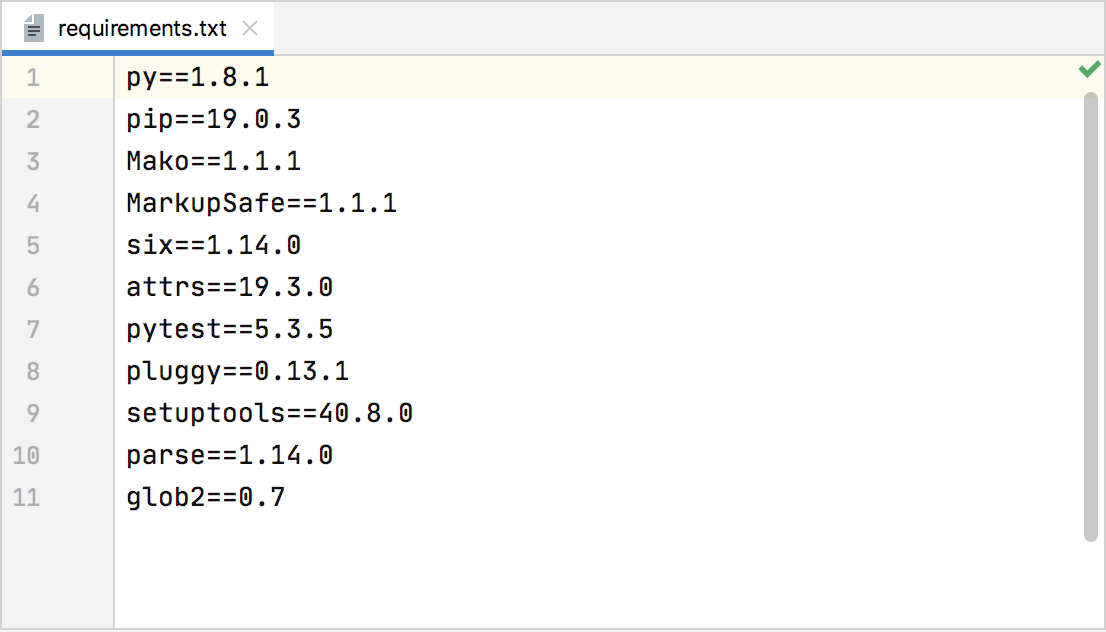
\includegraphics[scale=0.3]{author/part5/figures/pip.png}
	\caption{Файл конфигурации pip}
	\label{fig:pip}
\end{figure}

Пакетный менеджер pip хорошо работает с зависимостями, отображает безуспешно установленные пакеты, а также отображает информацию о требуемой версии пакета при конфликте с другим пакетом.

Альтернативой пакетного менеджера pip является пакетный менеджер poetry, который также ориентирован на язык программирования Python. Преимущество poetry перед pip в том, что он автоматически работает с виртуальными окружениями, способен самостоятельно их находить и создавать. Файл конфигурации для пакетов poetry является более богатым, чем у pip, он хранит такие сведения, как имя проекта, версия проекта, его описание, лицензия, список авторов, URL проекта, его документации и сайта, список ключевых слов проекта и список PyPI классификаторов. Poetry позволяет более гибко настраивать пакеты для проектов Python, файл конфигурации poetry представляет собой более богатую спецификацию проекта, однако эта спецификация не позволяет достичь совместимости между компонентами даже в рамках Python проектов и предназначена преимущественно только для чтения разработчиком. Автоматизировать проектирование компьютерных систем с помощью пакетного менеджера poetry или pip невозможно, так как требуется вмешательство разработчика, который должен вручную совместить интерфейсы устанавливаемых пакетов. Другие пакетные менеджеры языков программирования и операционных систем устроены по такому же принципу: существует хранилище компонентов (библиотека), которая представляет собой множество пакетов этого языка программирования или операционной системы и с которым взаимодействует менеджер компонентов.

\begin{figure}[H]
	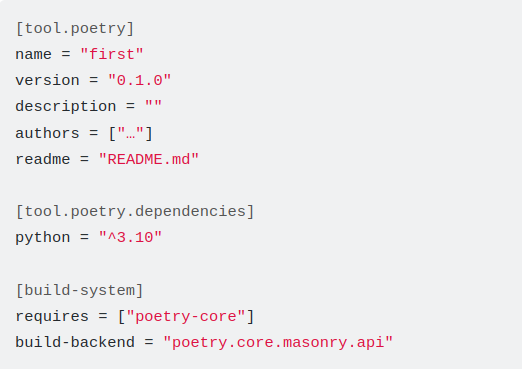
\includegraphics[scale=0.7]{author/part5/figures/poetry.png}
	\caption{Файл конфигурации poetry}
	\label{fig:poetry}
\end{figure}

В качестве компонентного подхода к проектированию программ можно рассмотреть библиотеки подпрограмм современных языков программирования, например, библиотеку стандартных шаблонов С++.

Библиотека стандартных шаблонов --- набор согласованных обобщённых алгоритмов, контейнеров, средств доступа к их содержимому и различных вспомогательных функций в C++.

В библиотеке выделяют пять основных компонентов:
\begin{textitemize}
	\item контейнер --- хранение набора объектов в памяти;
	\item итератор --- обеспечение средств доступа к содержимому контейнера;
	\item алгоритм --- определение вычислительной процедуры;
	\item адаптер --- адаптация компонентов для обеспечения различного интерфейса;
	\item функциональный объект --- сокрытие функции в объекте для использования другими компонентами.
\end{textitemize}

\begin{figure}[H]
	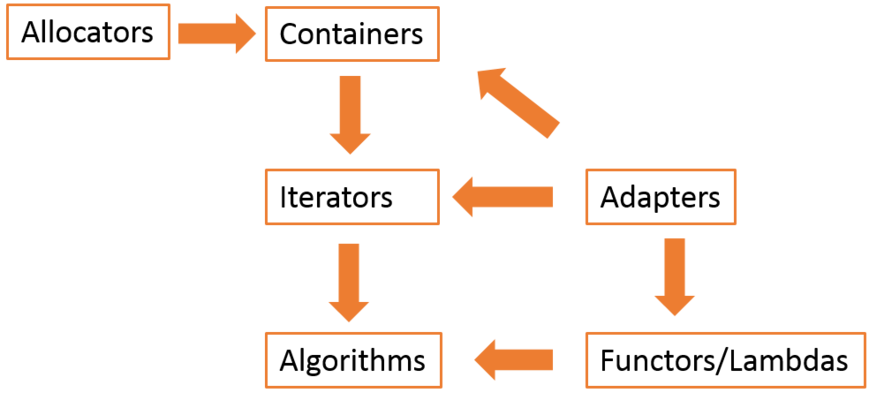
\includegraphics[scale=0.7]{author/part5/figures/STL.png}
	\caption{Структура библиотеки STL}
	\label{fig:STL}
\end{figure}

Разделение позволяет уменьшить количество компонентов. Например, вместо написания отдельной функции поиска элемента для каждого типа контейнера обеспечивается единственная версия, которая работает с каждым из них, пока соблюдаются основные требования.

Совместимость компонентов (контейнеров) в библиотеке стандартных шаблонов обеспечивается общим интерфейсом использования этих компонентов.

Компонентный подход к проектированию компьютерных систем может реализовываться в рамках различных языков, платформ и приложений. Рассмотрим некоторые из них.

Онтология, реализованная на языке OWL (Web Ontology Language), представляет собой множество декларативных утверждений о сущностях словаря предметной области (подробнее рассматривается в работе \scncite{Hepp2008}). OWL предполагает концепцию "открытого мира"{}, в соответствии с которой применимость описаний предметной области, помещённых в конкретном физическом документе, не ограничивается лишь рамками этого документа – содержание онтологии может быть использовано и дополнено другими документами, добавляющими новые факты о тех же сущностях или описывающими другую предметную область в терминах данной. "Открытость мира"{} достигается путём добавления URI каждому элементу онтологии, что позволяет воспринимать описанную на OWL онтологию как часть всеобщего объединённого знания.

\textbf{WebProtege} представляет собой многопользовательский веб-интерфейс, позволяющий редактировать и хранить онтологии в формате OWL в совместной среде (см. \scncite{Memduhoglu2018}). Данный проект позволяет не только создавать новые онтологии, но также загружать уже существующие онтологии, которые хранятся на сервере университета Стэнфорда. К преимуществу данного проекта можно отнести автоматическую проверку ошибок в процессе создания объектов онтологий. Данный проект является примером попытки решения проблемы накопления, систематизации и повторного использования уже существующих решений, однако, недостатком данного решения является обособленность разрабатываемых онтологий. Каждый разработанный компонент имеет свою иерархию понятий, подход к выделению классов и сущностей, которые зависят от разработчиков данных онтологий, так как в рамках данного подхода не существует универсальной модели представления знаний, а также формальной спецификации компонентов, представленных в виде онтологий. Следовательно, возникает проблема их семантической несовместимости, что, в свою очередь, приводит к невозможности повторного использования разработанных онтологий при проектировании баз знаний. Данный факт подтверждается наличием на сервере университета Стэнфорда многообразия различных онтологий на одни и те же темы.

На основе языка \textbf{Modelica} разработано большое число свободно доступных библиотек компонентов, одной из которых является библиотека Modelica\_StateGraph2, включающая компоненты для моделирования дискретных событий, реактивных и гибридных систем с помощью иерархических диаграмм состояния (см. \scncite{Fritzson2014}). Основным недостатком систем на базе языка Modelica является отсутствие совместимости компонентов и достаточной документации, а также узкая направленность разрабатываемых компонентов.

\textbf{Microsoft Power Apps} — это набор приложений, служб и соединителей, а также платформа данных, которая предоставляет среду разработки для эффективного создания пользовательских приложений для бизнеса. Платформа Power Apps имеет средства для создания библиотеки многократно используемых компонентов графического интерфейса, а также предварительно созданные модели распознавания текста (чтение визитных карточек или чеков) и средство обнаружение объектов, которые можно подключить к разрабатываемому приложению (см. \scncite{Prakash2022}). Библиотека компонентов Power Apps представляет собой множество создаваемых пользователем компонентов, которые можно использовать в любых приложениях. Преимущество библиотеки в том, что компоненты могут настраивать свойства по умолчанию, которые можно гибко редактировать в любых приложениях, использующих компоненты. Недостаток в том, что отсутствует семантическая совместимость компонентов, спецификация компонентов, не решена проблема существования семантически эквивалентных компонентов, нету иерархии компонентов и средств поиска этих компонентов. Компоненты платформы Microsoft Power Apps являются многократно используемыми только для однотипных приложений, которые создаются одним и тем же разработчиком.

\textbf{Платформа IACPaaS} (Intelligent Applications, Control and Platform as a Service, см. \scncite{Moskalenko2016}) – облачная платформа для разработки, управления и удаленного использования интеллектуальных облачных сервисов. Она предназначена для обеспечения поддержки разработки, управления и удаленного использования прикладных и инструментальных мультиагентных облачных сервисов (прежде всего интеллектуальных) и их компонентов для различных предметных областей. Платформа предоставляет доступ:
\begin{textitemize}
	\item прикладным пользователям (специалистам в различных предметных областях) - к прикладным сервисам;
	\item разработчикам прикладных и инструментальных сервисов и их компонентов - к инструментальным сервисам;
	\item управляющим интеллектуальными сервисами;
	\item к сервисам управления.
\end{textitemize}

Платформа IACPaaS поддерживает:

\begin{textitemize}
	\item базовую технологию разработки прикладных и специализированных инструментальных (интеллектуальных) сервисов с использованием базовыхинструментальных сервисов платформы, поддерживающих эту технологию;
	\item множество специализированных технологий разработки прикладных и специализированных инструментальных (интеллектуальных) сервисов, с использованием специализированных инструментальных сервисов платформы, поддерживающих эти технологии.
\end{textitemize}

Платформа IACPaaS также не имеет средств для унифицированного представления компонентов интеллектуальных компьютерных систем и средств для их спецификации и автоматической интеграции.

Исходя из проведённого анализа можно сказать, что на текущем состоянии развития информационных технологий не существует комплексной библиотеки многократно используемых семантически совместимых компонентов компьютерных систем. Таким образом, предлагается комплексная библиотека многократно используемых семантически совместимых компонентов ostis-систем.

\section{Комплексная библиотека многократно используемых семантически совместимых компонентов ostis-систем}
\label{ostis_library_section}

\begin{SCn}
\begin{scnrelfromlist}{ключевое понятие}
	\scnitem{материнская ostis-система}
	\scnitem{библиотека многократно используемых компонентов ostis-систем}
\end{scnrelfromlist}
\end{SCn}

\bigskip

\begin{SCn}
\begin{scnrelfromlist}{ключевое знание}
	\scnitem{архитектура Экосистемы OSTIS с точки зрения библиотек многократно используемых компонентов}
\end{scnrelfromlist}
\end{SCn}

\bigskip

Основным требованием, предъявляемым к \textit{Технологии OSTIS}, является обеспечение возможности совместного использования в рамках ostis-систем различных \textit{видов знаний} и различных \textit{моделей решения задач} с возможностью \myuline{неограниченного} расширения перечня используемых в ostis-системе видов знаний и моделей решения задач без существенных трудозатрат, а также различных видов интерфейсов. Следствием данного требования является необходимость реализации компонентного подхода на всех уровнях, от простых компонентов баз знаний, решателей задач и интерфейсов до целых встраиваемых ostis-систем (понятие компонента рассматривается далее в \ref{reusable_component_section}). Интеллектуальная система, спроектированная по Технологии OSTIS, представляет собой интеграцию многократно используемых компонентов баз знаний, многократно используемых компонентов решателей задач и многократно используемых компонентов интерфейсов (см. \scncite{Pivovarchik2015}). Различные многократно используемые компоненты ostis-систем объединяются в библиотеки многократно используемых компонентов ostis-систем. Разработчики \myuline{любой} ostis-системы могут включить в ее состав библиотеку, которая позволит им накапливать и распространять результаты своей деятельности среди других участников \textit{Экосистемы OSTIS} в виде \textbf{\textit{многократно используемых компонентов}}. Решение о включении компонента в библиотеку принимается экспертным сообществом разработчиков, ответственным за качество этой библиотеки. Верификацию компонентов можно автоматизировать путём проверки наличия обязательной части их спецификации, а также тестированием корректности автоматической установки и интеграции компонентов.

В рамках \textit{Экосистемы OSTIS} существует множество библиотек многократно используемых компонентов ostis-систем, являющихся подсистемами соответствующих материнских ostis-систем. Материнская ostis-система отвечает за какой-то класс компонентов и является САПРом для этого класса, содержит методики разработки таких компонентов, их классификацию, подробные пояснения ко всем подклассам компонентов. Таким образом, формируется иерархия \textbf{\textit{материнских ostis-систем}}. Материнская ostis-система в свою очередь может являться дочерней ostis-системой для какой-либо другой ostis-системы, заимствуя компоненты из библиотеки, входящей в состав этой другой ostis-системы.

\begin{SCn}
	\scnheader{ostis-система}
	\scnsuperset{материнская ostis-система}
	\begin{scnindent}
		\scnidtf{ostis-система, имеющая в своем составе библиотеку многократно используемых компонентов.}
		\scnhaselement{Метасистема OSTIS}
	\end{scnindent}
	\scnsuperset{дочерняя ostis-система}
	\begin{scnindent}
		\scnidtf{ostis-система, в составе которой имеется компонент, заимствованный из какой-либо библиотеки многократно используемых компонентов.}
	\end{scnindent}
\end{SCn}

Библиотека многократно используемых компонентов ostis-систем позволяет использовать проектный опыт по разработке и модернизации ostis-систем различного назначения.

\begin{SCn}
	\scnheader{библиотека многократно используемых компонентов ostis-систем}
	\scntext{часто используемый sc-идентификатор}{библиотека компонентов ostis-систем}
	\scntext{часто используемый sc-идентификатор}{библиотека компонентов}
	\scnidtf{комплексная библиотека многократно используемых семантически совместимых компонентов ostis-систем}
	\scnidtf{библиотека многократно используемых и совместимых компонентов интеллектуальных компьютерных систем нового поколения}
	\scnidtf{библиотека типовых компонентов ostis-систем}
	\scnidtf{библиотека многократно используемых компонентов OSTIS}
	\scnidtf{библиотека повторно используемых компонентов OSTIS}
	\scnidtf{библиотека intelligent property компонентов ostis-систем}
	\begin{scnindent}
		\scntext{сокращение}{библиотека ip-компонентов ostis-систем}
	\end{scnindent}
	\scnhaselementrole{типичный пример}{\scnkeyword{Библиотека OSTIS}}
	\begin{scnindent}
		\scnidtf{Распределенная библиотека типовых (многократно используемых) компонентов ostis-систем}
		\scnidtf{Библиотека многократно используемых компонентов ostis-систем в составе Метасистемы OSTIS}
		\scnidtf{Библиотека Метасистемы OSTIS}
	\end{scnindent}
	\begin{scnreltoset}{объединение}
		\scnitem{библиотека многократно используемых компонентов баз знаний (см. \textit{\ref{sc_kb_design_components}~\nameref{sc_kb_design_components})}}
		\scnitem{библиотека многократно используемых компонентов решателей задач (см. \textit{\ref{ps_components_section}~\nameref{ps_components_section})}}
		\scnitem{библиотека многократно используемых компонентов пользовательских интерфейсов (см. \textit{ \ref{sec_reusable_UI_components}~\nameref{sec_reusable_UI_components})}}
		\scnitem{библиотека встраиваемых ostis-систем}
		\scnitem{библиотека ostis-платформ}
	\end{scnreltoset}
\end{SCn}

Главной библиотекой многократно используемых компонентов ostis-систем является \textit{Библиотека Метасистемы OSTIS}. \textit{Метасистема OSTIS} (см. Главу \textit{\ref{chapter_ims_standard}~\nameref{chapter_ims_standard}}) выступает \textbf{\textit{материнской системой}} для всех разрабатываемых ostis-систем, поскольку содержит все базовые компоненты (рисунок \textit{\nameref{fig:ecosystem_architecture}}).

\begin{figure}[H]
	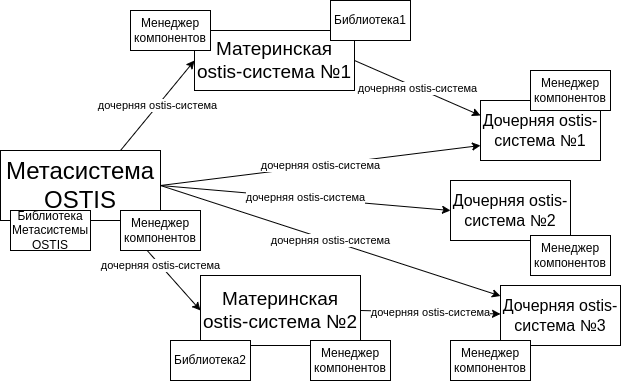
\includegraphics[scale=0.8]{author/part5/figures/ecosystem_architecture.png}
	\caption{Архитектура Экосистемы OSTIS с точки зрения библиотек многократно используемых компонентов}
	\label{fig:ecosystem_architecture}
\end{figure}

% Понятие ябиблиотеки OSTIS
Основу для реализации компонентного подхода в рамках \textit{Технологии OSTIS} составляет \textbf{\textit{Библиотека OSTIS}}. \textit{Метасистема OSTIS} ориентирована на разработку и практическое внедрение методов и средств компонентного проектирования семантически совместимых интеллектуальных систем, которая предоставляет возможность быстрого создания интеллектуальных систем различного назначения. В состав Метасистемы OSTIS входит \textbf{\textit{Библиотека OSTIS}}. Сферы практического применения технологии компонентного проектирования семантически совместимых интеллектуальных систем ничем не ограничены.

% Зачем нужна Библиотека OSTIS
Основное назначение Библиотеки OSTIS --- создание условий для эффективного, осмысленного и массового проектирования ostis-систем и их компонентов путём создания среды для накопления и совместного использования компонентов ostis-систем. Такие условия осуществляются путём неограниченного расширения постоянно эволюционируемых семантически совместимых ostis-систем и их компонентов, входящих в \textit{Экосистему OSTIS}.

Постоянно расширяемая Библиотека OSTIS существенно сокращает сроки разработки новых интеллектуальных компьютерных систем.
библиотека многократно используемых компонентов ostis-систем позволяет избавиться от дублирования семантически эквивалентных информационных компонентов. А также от многообразия форм технической реализации используемых моделей решения задач.

% Что умеет библиотека ostis-систем
Функциональные возможности библиотеки многократно используемых компонентов ostis-систем (см. \scncite{Koronchik2011}):
\begin{SCn}
	\scnheader{библиотека многократно используемых компонентов ostis-систем}
	\begin{scnrelfromset}{функциональные возможности}
		\scnfileitem{Хранение многократно используемых компонентов ostis-систем и их спецификаций. При этом часть компонентов, специфицированных в рамках библиотеки, могут физически храниться в другом месте ввиду особенностей их  технической реализации (например, исходные тексты ostis-платформы могут физически храниться в каком-либо отдельном репозитории, но специфицированы как компонент будут в соответствующей библиотеке). В этом случае спецификация компонента в рамках библиотеки должна также включать описание (1) того \myuline{где} располагается компонент и (2) сценария его \myuline{автоматической} установки в дочернюю ostis-систему.}
		\scnfileitem{Просмотр имеющихся компонентов и их спецификаций, а также поиск компонентов по фрагментам их спецификации.}
		\scnfileitem{Хранение сведений о статистике использования компонентов. Например, в каких ostis-системах-потребителях какие из компонентов библиотеки и какой версии используются (были скачаны). Это необходимо для учета востребованности того или иного компонента, оценки его важности и популярности.}
		\scnfileitem{Систематизация многократно используемых компонентов ostis-систем.}
		\scnfileitem{Обеспечение версионирования многократно используемых компонентов ostis-систем.}
		\scnfileitem{Поиск зависимостей между многократно используемыми компонентами в рамках библиотеки компонентов.}
		\scnfileitem{Обеспечение автоматического обновления компонентов, заимствованных в дочерние ostis-системы. Данная функция может включаться и отключаться по желанию разработчиков дочерней ostis-системы. Одновременное обновление одних и тех же компонентов во всех системах, его использующих, не должно \myuline{ни в каком контексте} приводить к несогласованности между этими системами. Это требование может оказаться довольно сложным, но без него работа Экосистемы OSTIS невозможна.}
	\end{scnrelfromset}
\end{SCn}

\textit{\textbf{библиотека многократно используемых компонентов ostis-систем}} является подсистемой ostis-систем, которая имеет свою базу знаний, свой решатель задач и свой интерфейс. Однако не каждая ostis-система обязана иметь библиотеку.

\begin{SCn}
	\scnheader{библиотека многократно используемых компонентов ostis-систем}
	\begin{scnrelfromset}{обобщенная декомпозиция}
		\scnitem{база знаний библиотеки многократно используемых компонентов ostis-систем}
		\scnitem{решатель задач библиотеки многократно используемых компонентов ostis-систем}
		\scnitem{интерфейс библиотеки многократно используемых компонентов ostis-систем}
		\begin{scnindent}
			\begin{scnrelfromset}{декомпозиция}
				\scnitem{минимальный интерфейс библиотеки многократно используемых компонентов ostis-систем}
				\scnitem{расширенный интерфейс библиотеки многократно используемых компонентов ostis-систем}
				\begin{scnindent}
					\scnidtf{графический интерфейс библиотеки многократно используемых компонентов ostis-систем}
					\scnrelfrom{включение}{SCg-интерфейс библиотеки многократно используемых компонентов ostis-систем}
				\end{scnindent}
			\end{scnrelfromset}
		\end{scnindent}
	\end{scnrelfromset}
\end{SCn}

\textit{\textbf{решатель задач библиотеки многократно используемых компонентов ostis-систем}} реализует функциональные возможности библиотеки ostis-систем.

\textit{\textbf{база знаний библиотеки мнoгократно используемых компонентов ostis-систем}} представляет собой иерархию многократно используемых компонентов ostis-систем и их спецификаций.

\textit{\textbf{интерфейс библиотеки многократно используемых компонентов ostis-систем}} обеспечивает доступ к многократно используемым компонентам и возможностям библиотеки ostis-систем для пользователя и других систем (см. \scncite{Koronchik2011}). Существует минимальный и расширенный интерфейс библиотеки многократно используемых компонентов ostis-систем. Минимальный интерфейс позволяет \textit{менеджеру многократно используемых компонентов ostis-систем}, входящему в состав какой-либо дочерней ostis-системы, подключиться к библиотеке многократно используемых компонентов ostis-систем и использовать ее функциональные возможности, то есть, например, получить доступ к спецификации компонентов и установить выбранные компоненты в дочернюю ostis-систему, получить сведения до доступных версиях компонента, его зависимостях и так далее. Расширенный интерфейс, в отличие от минимального интерфейса, позволяет не только получить доступ к компонентам для дальнейшей работы с ними, но и просматривать существующую структуру библиотеки, а также компоненты и их элементы в удобном и интуитивно понятном для пользователя виде.

% Как происходит интеграция компонентов
Проблема интеграции многократно используемых компонентов ostis-систем решается путём взаимодействия компонентов через общую базу знаний. Компоненты могут лишь использовать общие ключевые узлы (понятия) в базе знаний (см. \scncite{Davydenko2013}, \scncite{Ivashenko2013} и \scncite{Golenkov2014b}). Интеграция многократно используемых компонентов ostis-систем сводится к отождествлению ключевых узлов (см. \ref{sec_ontological_formalization_basic_denotational_semantics_sc-code}~\nameref{sec_ontological_formalization_basic_denotational_semantics_sc-code}) и устранению возможных дублирований и противоречий исходя из спецификации компонента и его содержания. Такой способ интеграции компонентов позволяет разрабатывать их параллельно и независимо друг от друга, что значительно сокращает сроки проектирования. Отождествление sc-элементов происходит в ходе выполнения \textit{действие. отождествить два указанных sc-элемента}, которое рассматривается в главе \ref{chapter_situation_management} Автоматическая интеграция компонентов интеллектуальных систем представляет широкие возможности для существенного сокращения сроков проектирования интеллектуальных систем, поскольку позволяет использовать опыт прошлых разработок.

Рассмотрим пример интеграции многократно используемого компонента решателя задач, который представляет собой sc-агент поиска кратчайшего пути в графе, в систему управления логистическими процессами. Допустим, система управления логистическими процессами умеет решать задачи, связанные с оптимизацией издержек в процессе создания товара и со складированием товаров. 

\begin{figure}[H]
	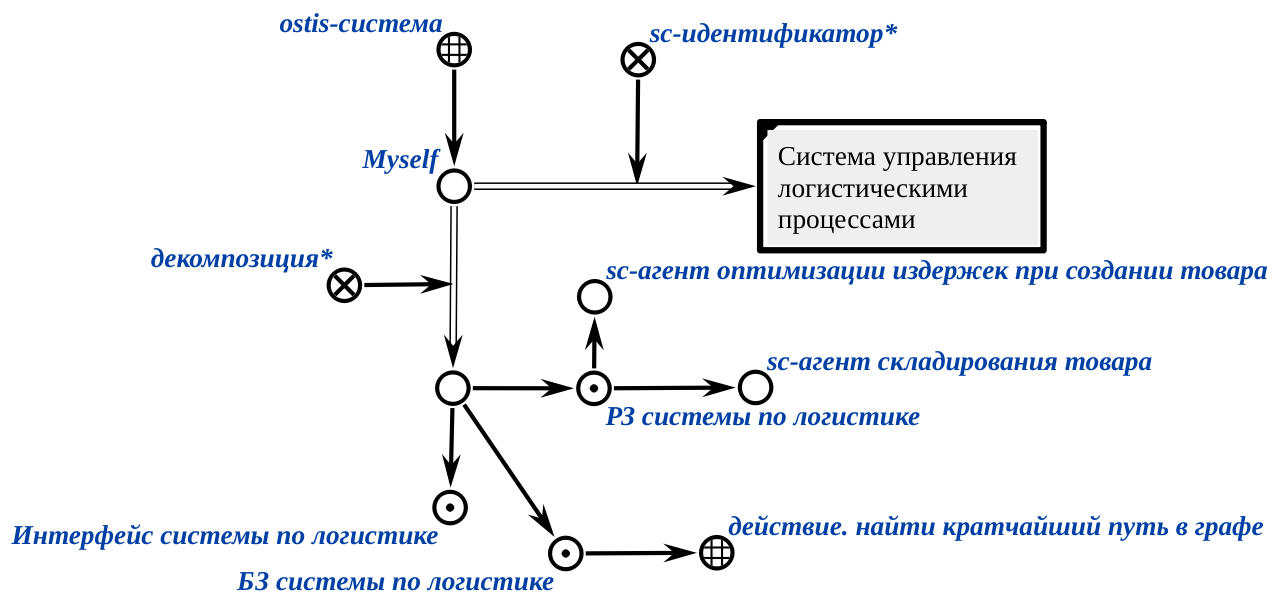
\includegraphics[scale=0.5]{author/part5/figures/logistics_system.png}
	\caption{Структура системы управления логистическими процессами}
	\label{fig:logistics_system}
\end{figure}

При этом в базе знаний системы описано, какие задачи должна решать система и соответствующие им действия. Например, действие. найти кротчайший путь в графе, которое система пока что не умеет выполнять.

Система решения задач по теории графов имеет богатую базу знаний и решатель задач, в том числе имеет sc-агент поиска кратчайшего пути в графе, который специфицирован как многократно используемый компонент и может быть использован в системе по логистике.

\begin{figure}[H]
	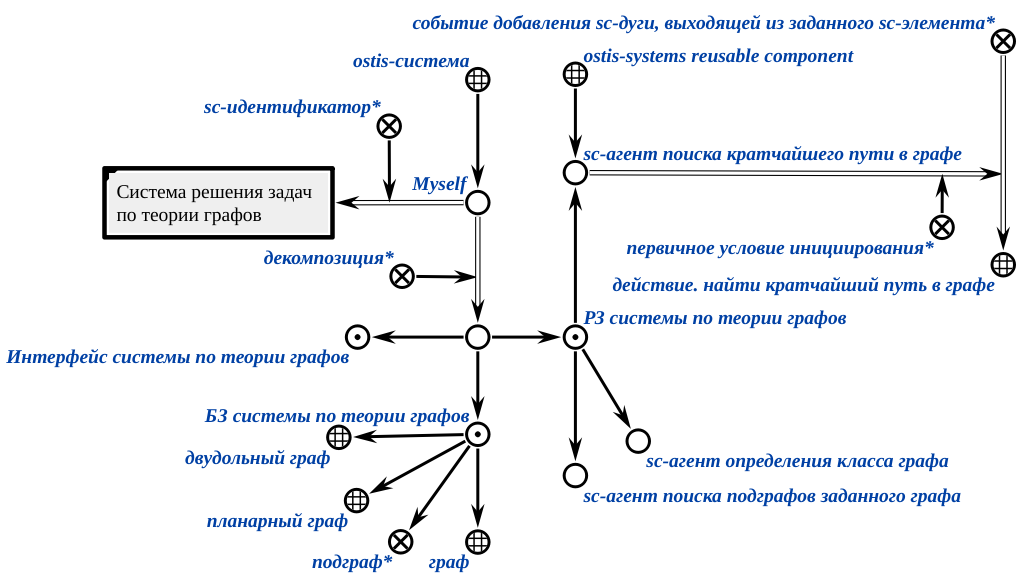
\includegraphics[scale=0.4]{author/part5/figures/graph_theory_system.png}
	\caption{Структура системы решения задач по теории графов}
	\label{fig:graph_theory_system}
\end{figure}

В результате установки многократно используемого компонента в виде sc-агента поиска кратчайшего пути в графе вся его sc-модель погружается в систему решения задач по логистике. При интеграции многократно используемого компонента, который представляет собой sc-агент поиска кратчайшего пути в графе, в систему по логистике ключевой узел \textit{действие. найти кратчайший путь в графе} системы по логистике отождествляется с таким же узлом из установленного компонента из системы по теории графов. Таким образом, при выполнении логистических задач, система сможет интерпретировать действие по поиску кратчайших путей с помощью интегрированного компонента.

% Кто ещё говорит про интеграцию фрагментов БЗ? В главе Сашеньки не рассматривается. В смысловом пространстве? 
Интеграция любых компонентов ostis-систем происходит автоматически, \myuline{без} вмешательства разработчика. Это достигается за счёт использования \textit{SC-кода} и его преимуществ, унификации спецификации многократно используемых компонентов и тщательного отбора компонентов в библиотеках экспертным сообществом, ответственным за эту библиотеку.

\section{Понятие многократно используемого компонента ostis-систем}
\label{reusable_component_section}

\begin{SCn}
	\begin{scnrelfromlist}{ключевое понятие}
		\scnitem{многократно используемый компонент ostis-систем}
	\end{scnrelfromlist}
\end{SCn}

\bigskip

\begin{SCn}
	\begin{scnrelfromlist}{ключевое знание}
		\scnitem{классификация многократно используемых компонентов ostis-систем}
		\scnitem{спецификация многократно используемых компонентов ostis-систем}
	\end{scnrelfromlist}
\end{SCn}

Рассмотрим понятие многократно используемого компонента ostis-систем. Под многократно используемым компонентом ostis-систем понимается  компонент некоторой ostis-системы, который может быть использован в рамках другой ostis-системы (см. \scncite{Shunkevich2015a}). Это компонент ostis-системы, который может быть использован в других ostis-системах (\textbf{\textit{дочерних ostis-системах}}) и содержит все те и только те sc-элементы, которые необходимы для функционирования компонента в дочерней ostis-системе. Другими словами это компонент некоторой \textbf{\textit{материнской ostis-системы}}, который может быть использован в некоторой дочерней ostis-системе. Для включения многократно используемого компонента в некоторую систему, его необходимо установить в эту систему, то есть скопировать в неё все sc-элементы компонента и, при необходимости, вспомогательные файлы, такие как исходные или скомпилированные файлы компонента. Многократно используемые компоненты должны иметь унифицированную спецификацию и иерархию для поддержки \myuline{совместимости} с другими компонентами. Совместимость многократно используемых компонентов приводит систему к новому качеству, к дополнительному расширению множества решаемых задач при интеграции компонентов.

\begin{SCn}
	\scnheader{многократно используемый компонент ostis-систем}
	\scnidtf{типовой компонент ostis-систем}
	\scnidtf{повторно используемый компонент ostis-систем}
	\scnidtf{многократно используемый компонент OSTIS}
	\scnidtf{ip-компонент ostis-систем}
	\scnidtftext{часто используемый sc-идентификатор}{многократно используемый компонент}
	\scnsubset{компонент ostis-системы}
	\scnsubset{sc-структура}
\end{SCn}

\textit{\textbf{компонент ostis-системы}} --- это целостная часть ostis-системы, которая содержит все те (и только те) sc-элементы, которые необходимы для её функционирования в ostis-системе. многократно используемый компонент ostis-систем --- это общий компонент (общая часть) для некоторого множества ostis-систем, который многократно используется, дублируется и входит в состав некоторого множества ostis-систем.
Отличие многократно используемого компонента ostis-систем от компонента ostis-системы в том, что многократно используемый компонент имеет \myuline{спецификацию, достаточную для установки} этого компонента в дочернюю ostis-систему. Спецификация является частью базы знаний библиотеки многократно используемых компонентов соответствующей материнской ostis-системы. Есть техническая возможность встроить многократно используемый компонент в дочернюю ostis-систему.

Требования, предъявляемые к многократно используемым компонентам ostis-систем, наследуют общие требования к проектированию программных компонентов, а также включают следующие:
\begin{textitemize}
	\item существует техническая возможность встроить многократно используемый компонент в дочернюю ostis-систему;
	\item многократно используемый компонент должен выполнять свои функции наиболее общим образом, чтобы круг возможных систем, в которые он может быть встроен, был наиболее широким;
	\item совместимость многократно используемого компонента: компонент должен стремиться повышать уровень \myuline{договороспособности} ostis-систем, в которые он встроен и иметь возможность \myuline{автоматической} интеграции в другие системы;
	\item самодостаточность компонентов (или групп компонентов) технологии, то есть способности их функционировать отдельно от других компонентов без утраты целесообразности их использования.
\end{textitemize}

Рассмотрим классификацию многократно используемых компонентов ostis-систем (см. \scncite{Shunkevich2015a}). Класс многократно используемого компонента ostis-систем является важной частью спецификации компонента, позволяющей лучше понять назначение и область применения данного компонента, а также класс многократно используемого компонента является важнейшим критерием поиска компонентов в библиотеке ostis-систем. Основной признак классификации многократно используемых компонентов является признак предметной области, к которой относится компонент. Здесь структура может быть довольно богатой в соответствии с иерархией областей человеческой деятельности.

\begin{SCn}
\scnheader{многократно используемый компонент ostis-систем}
\begin{scnrelfromset}{разбиение}
	\scnitem{многократно используемый компонент базы знаний}
	\begin{scnindent}
		\scnsuperset{семантическая окрестность}
		\begin{scnindent}
			\scnhaselement{Семантическая окрестность города Минска}
			\scnhaselement{Семантическая окрестность понятия множество}
		\end{scnindent}
		\scnsuperset{предметная область и онтология}
		\begin{scnindent}
			\scnhaselement{Предметная область и онтология треугольников}
		\end{scnindent}
		\scnsuperset{шаблон многократно используемого компонента ostis-систем}
		\begin{scnindent}
			\scnhaselement{Шаблон описания предметной области}
			\scnhaselement{Шаблон описания отношения}
		\end{scnindent}
	\end{scnindent}
	\scnitem{многократно используемый компонент решателя задач}
	\begin{scnindent}
		\scnsuperset{атомарный абстрактный sc-агент}
		\begin{scnindent}
			\scnhaselement{Абстрактный sc-агент подсчёта мощности множества}
		\end{scnindent}
		\scnsuperset{программа обработки знаний}
		\scnsuperset{scp-машина}
		\scnsuperset{scl-машина}
	\end{scnindent}
	\scnitem{многократно используемый компонент интерфейса}
	\begin{scnindent}
		\scnsuperset{многократно используемйы компонент пользовательского интерфейса для отображения}
		\scnsuperset{интерактивный многократно используемый компонент пользовательского интерфейса}
	\end{scnindent}
\end{scnrelfromset}
\end{SCn}	

На рисунке \nameref{fig:set_neighbourhood} приведён фрагмент многократно используемого компонента базы знаний на примере семантической окрестности понятия \textit{множество}.

\begin{figure}[H]
	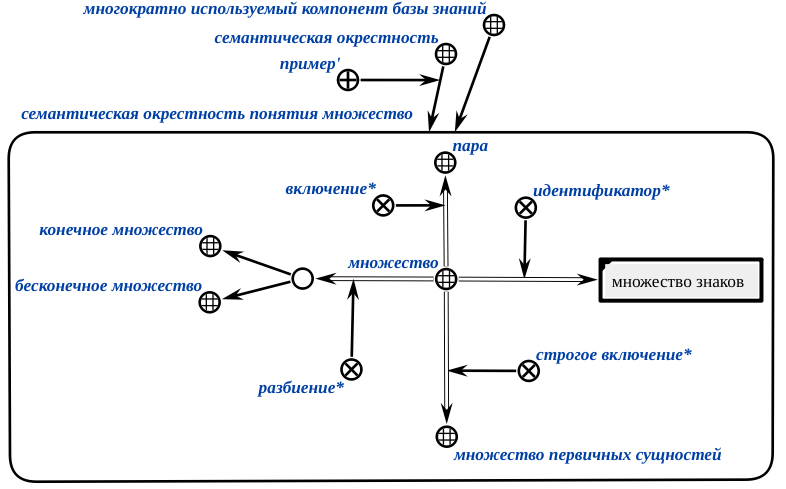
\includegraphics[scale=0.6]{author/part5/figures/set_neighbourhood.png}
	\caption{Пример многократно используемого компонента базы знаний}
	\label{fig:set_neighbourhood}
\end{figure}

На рисунке \nameref{fig:relation_template} приведён фрагмент шаблона многократно используемого компонента ostis-систем на примере описания семантической окрестности отношения. Шаблоны многократно используемых компонентов также можно использовать для описания платформенно-независимых компонентов решателя задач и интерфейсов.

\begin{figure}[H]
	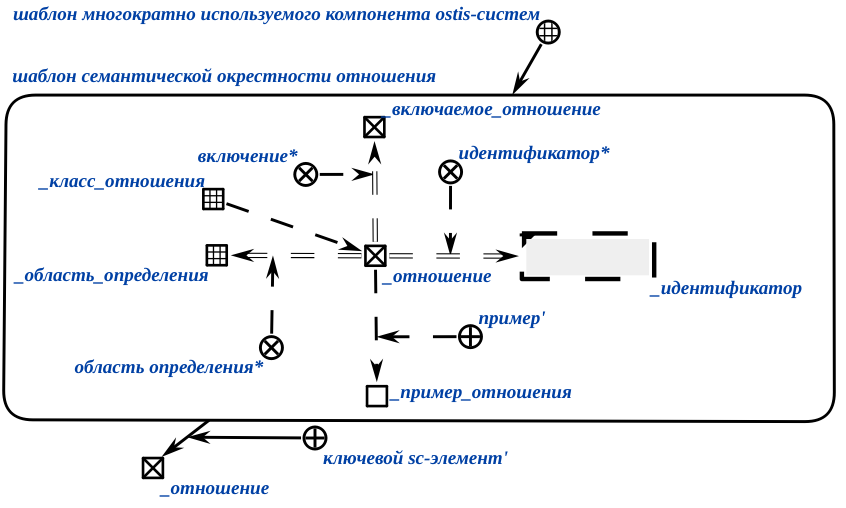
\includegraphics[scale=0.6]{author/part5/figures/relation_template.png}
	\caption{Пример шаблона семантической окрестности отношения}
	\label{fig:relation_template}
\end{figure}

Для компонентов баз знаний важнейшим признаком классификации многократно используемых компонентов является \textbf{\textit{вид используемых знаний}}. Для компонентов решателя задач --- \textbf{\textit{модель решения задач}}. Для компонентов интерфейса --- \textbf{\textit{вид интерфейса}} в соответствии с классификацией компонентов пользовательских интерфейсов.

\begin{SCn}
\scnheader{многократно используемый компонент ostis-систем}
\scnrelfrom{разбиение}{\scnkeyword{Типология компонентов ostis-систем по атомарности\scnsupergroupsign}}
\begin{scnindent}
	\begin{scneqtoset}
		\scnitem{атомарный многократно используемый компонент ostis-систем}
		\begin{scnindent}
			\scnhaselement{Абстрактный sc-агент подсчёта мощности множества}
		\end{scnindent}
		\scnitem{неатомарный многократно используемый компонент ostis-систем}
		\begin{scnindent}
			\scnidtf{составной многократно используемый компонент ostis-систем}
			\scnhaselement{Решатель задач по геометрии}
		\end{scnindent}
	\end{scneqtoset}
\end{scnindent}
\end{SCn}

\textbf{\textit{атомарный многократно используемый компонент ostis-систем}} --- это компонент, который в текущем состоянии библиотеки ostis-систем рассматривается как неделимый, то есть не содержит в своем составе других компонентов. Принадлежность многократно используемого компонента ostis-систем классу атомарных компонентов зависит от того, как специфицирован этот компонент и от существующих на данный момент компонентов в библиотеке. Неатомарный многократно используемый компонент в текущем состоянии библиотеки ostis-систем содержит в своем составе другие атомарные или неатомарные компоненты, он не зависит от своих частей. Без какой-либо части неатомарного компонента его назначение сужается. В общем случае атомарный компонент может перейти в разряд неатомарных в случае, если будет принято решение выделить какую-то из его частей в качестве отдельного компонента. Все вышесказанное, однако, не означает, что даже в случае его платформенной независимости, атомарный компонент всегда хранится в sc-памяти как сформированная sc-структура. Например, платформенно-независимая реализация sc-агента всегда будет представлена набором scp-программ, но будет атомарным многократно используемым компонентом OSTIS в случае, если ни одна из этих программ не будет представлять интереса как самостоятельный компонент. В общем случае неатомарный компонент может перейти в разряд атомарных в случае, если будет принято решение по каким-либо причинам исключить все его части из рассмотрения в качестве отдельных компонентов. Следует отметить, что неатомарный компонент необязательно должен складываться \myuline{полностью} из других компонентов, в его состав могут также входить и части, не являющиеся самостоятельными компонентами. Например, в состав реализованного на языке SCP sc-агента, являющего неатомарным многократно используемым компонентом могут входить как scp-программы, которые могут являться многократно используемыми компонентами (а могут и не являться), а также агентная scp-программа, которая не имеет смысла как многократно используемый компонент.

\begin{SCn}
\scnheader{многократно используемый компонент ostis-систем}
\scnrelfrom{разбиение}{\textbf{\textit{Типология компонентов ostis-систем по зависимости\scnsupergroupsign}}}
\begin{scnindent}
	\begin{scneqtoset}
		\scnitem{зависимый многократно используемый компонент ostis-систем}
		\begin{scnindent}
			\scnhaselement{визуальный редактор системы по химии}
		\end{scnindent}
		\scnitem{независимый многократно используемый компонент ostis-систем}
		\begin{scnindent}
			\scnhaselement{предметная область чисел}
		\end{scnindent}
	\end{scneqtoset}
\end{scnindent}
\end{SCn}

\textbf{\textit{зависимый многократно используемый компонент ostis-систем}} зависит хотя бы от одного другого компонента библиотеки ostis-систем и не может функционировать в дочерней ostis-системе без компонентов, от которых он зависит. \textit{независимый многократно используемый компонент ostis-систем} не зависит ни от одного другого компонента библиотеки ostis-систем.

\begin{SCn}
\scnheader{многократно используемый компонент ostis-систем}
\scnrelfrom{разбиение}{\scnkeyword{Типология компонентов ostis-систем по способу их хранения\scnsupergroupsign}}
\begin{scnindent}
	\begin{scneqtoset}
		\scnitem{многократно используемый компонент ostis-систем, хранящийся в виде внешних файлов}
		\begin{scnindent}
			\begin{scnrelfromset}{разбиение}
				\scnitem{многократно используемый компонент ostis-систем, хранящийся в виде файлов исходных текстов}
				\scnitem{многократно используемый компонент ostis-систем, хранящийся в виде скомпилированных файлов}
			\end{scnrelfromset}
		\end{scnindent}
		\scnitem{многократно используемый компонент, хранящийся в виде sc-структуры}
	\end{scneqtoset}
\end{scnindent}
\end{SCn}

На данном этапе развития \textit{Технологии OSTIS} более удобным является хранение компонентов в виде исходных текстов.

\begin{SCn}
\scnheader{многократно используемый компонент ostis-систем}
\scnrelfrom{разбиение}{\scnkeyword{Типология компонентов ostis-систем по зависимости от ostis-платформы\scnsupergroupsign}}
\begin{scnindent}
	\begin{scneqtoset}
		\scnitem{платформенно-зависимый многократно используемый компонент ostis-систем}
		\begin{scnindent}
			\scnsuperset{ostis-платформа}
			\scnsuperset{абстрактный sc-агент, не реализуемый на Языке SCP}
		\end{scnindent}
		\scnitem{платформенно-независимый многократно используемый компонент ostis-систем}
		\begin{scnindent}
			\scnsuperset{многократно используемый компонент базы знаний}
			\scnsuperset{платформенно-независимый абстрактный sc-агент}
			\scnsuperset{scp-программа}
		\end{scnindent}
	\end{scneqtoset}
\end{scnindent}
\end{SCn}

Под \textbf{\textit{платформенно-зависимым многократно используемым компонентом ostis-систем}} понимается компонент, частично или полностью реализованный при помощи каких-либо сторонних с точки зрения \textit{Технологии OSTIS} средств. Недостаток таких компонентов в том, что интеграция таких компонентов в интеллектуальные системы может сопровождаться дополнительными трудностями, зависящими от конкретных средств реализации компонента. В качестве возможного преимущества платформенно-зависимых многократно используемых компонентов ostis-систем можно выделить их, как правило, более высокую производительность за счет реализации их на более приближенном к платформе уровне. В общем случае платформенно-зависимый многократно используемый компонент ostis-систем может поставляться как в виде набора исходных кодов, так и скомпилированном виде. Процесс интеграции платформенно-зависимого многократно используемого компонента ostis-систем в дочернюю систему, разработанную по Технологии OSTIS, сильно зависит от технологий реализации данного компонента и в каждом конкретном случае может состоять из различных этапов. Каждый платформенно-зависимый многократно используемый компонент ostis-систем должен иметь соответствующую подробную, корректную и понятную инструкцию по его установке и внедрению в дочернюю систему.

Под \textbf{\textit{платформенно-независимым многократно используемым компонентом ostis-систем}} понимается компонент, который целиком и полностью представлен на \textit{SC-коде}. В случае неатомарного многократно используемого компонента это означает, что все более простые компоненты, входящие в его состав также обязаны быть платформенно-независимыми многократно используемыми компонентами ostis-систем. Процесс интеграции платформенно-зависимого многократно используемого компонента ostis-систем в дочернюю систему, разработанную по Технологии OSTIS, существенно упрощается за счет использования общей унифицированной формальной основы представления и обработки знаний.

Наиболее ценными являются платформенно-независимые многократно используемые компоненты ostis-систем.

\begin{SCn}
\scnheader{многократно используемый компонент ostis-систем}
\scnrelfrom{разбиение}{\scnkeyword{Типология компонентов ostis-систем по динамичности их установки\scnsupergroupsign}}
\begin{scnindent}
	\begin{scneqtoset}
		\scnitem{динамически устанавливаемый многократно используемый компонент ostis-систем}
		\begin{scnindent}
			\scnidtf{многократно используемый компонент, при установке которого система не требует перезапуска}
			\begin{scnrelfromset}{декомпозиция}
				\scnitem{многократно используемый компонент, хранящийся в виде скомпилированных файлов}
				\scnitem{многократно используемый компонент базы знаний}
			\end{scnrelfromset}
		\end{scnindent}
		\scnitem{многократно используемый компонент, при установке которого система требует перезапуска}
	\end{scneqtoset}
\end{scnindent}
\end{SCn}

Процесс интеграции компонентов разных видов на разных этапах жизненного цикла osits-систем бывает разным. Наиболее ценными являются компоненты, которые могут быть интегрированы в работающую систему \myuline{без} прекращения её функционирования. Некоторые системы, особенно системы управления, нельзя останавливать, а устанавливать и обновлять компоненты нужно.

\textbf{\textit{встраиваемая ostis-система}} --- это неатомарный многократно используемый компонент, который состоит из базы знаний, решателя задач и интерфейса.

\begin{SCn}
	\scnheader{встраиваемая ostis-система}
	\scnsubset{ostis-система}
	\scnsubset{неатомарный многократно используемый компонент ostis-систем}
	\begin{scnrelfromset}{декомпозиция}
		\scnitem{многократно используемый компонент базы знаний}
		\scnitem{многократно используемый компонент решателя задач}
		\scnitem{многократно используемый компонент интерфейса}
	\end{scnrelfromset}
\end{SCn}

Такими системами могут быть, например, интеллектуальный интерфейс (в том числе естественно-языковой интерфейс), среда коллективного проектирования баз знаний, менеджер многократно используемых компонентов ostis-систем, обучающая система, система тестирования и верификации интеллектуальных систем, визуальный web-ориентированный редактор sc.g-текстов и другие.

Особенность встраиваемых систем в том, что интеграция целых интеллектуальных систем предполагает интеграцию баз знаний этих систем, интеграцию их решателей задач и интеграцию их интеллектуальных интерфейсов. При интеграции встраиваемых систем база знаний встраиваемой системы становится частью базы знаний системы, в которую она встраивается. Решатель задач встраиваемой системы становится частью решателя задач системы, в которую она встраивается. И интерфейс встраиваемой системы становится частью интерфейса системы, в которую она встраивается. При этом встраиваемая система является целостной и может функционировать отдельно от других ostis-систем, в отличие от других многократно используемых компонентов.

Встраиваемые ostis-системы зачастую являются предметно независимыми. Таким образом, например, встраиваемая система в виде среды проектирования баз знаний может быть встроена как в систему из предметной области по геометрии, так и в систему управления аграрными объектами.

Встраиваемя ostis-система, как и любой другой многократно используемый компонент ostis-систем, должна поддерживать семантическую совместимость ostis-систем. Как сама встраиваемая ostis-система, так и все её компоненты должны быть специфицированы и согласованы. Компоненты встраиваемых ostis-систем могут быть заменены на другие, имеющие то же назначение, например, естественно-языковой интерфейс может иметь различные варианты базы знаний в зависимости от естественного языка, поддерживаемого системой, различные варианты пользовательского интерфейса, в зависимости от требований и удобства пользователей и также различные варианты реализации решателя задач для обработки естественного языка, которые могут использовать различные модели, однако решать одну и ту же задачу. Встраиваемая ostis-система связывается с системой, в которую она встроена с помощью отношения \textit{\textbf{встраиваемая ostis-система*}}.

Для того, чтобы хранить многократно используемые компоненты ostis-систем, необходимо некоторое хранилище. Таким хранилищем может выступать как какая-либо ostis-система, так и стороннее хранилище, например, облачное. Помимо внешних файлов компонента в хранилище должна находиться его \myuline{спецификация}.

Каждый \textit{многократно используемый компонент ostis-систем} должен быть специфицирован в рамках библиотеки (см. \scncite{Davydenko2013}). Данные спецификации включают в себя основные знания о компоненте, которые позволяют обеспечить построение полной иерархии компонентов и их зависимостей, а также обеспечивают \myuline{беспрепятственную} интеграцию компонентов в дочерние ostis-системы. Для спецификации компонента используются, как отношения, так и классы компонента.

% Параметры формализовать
Чтобы многократно используемый компонент мог быть принят в библиотеку, нужно специфицировать его, используя отношения класса \textit{необходимое для установки отношение, специфицирующее многократно используемый компонент ostis-систем}. Здесь описана спецификация, общая для любых типов компонентов, однако в зависимости от типа компонента, спецификация может расширяться (см. \textit{\ref{sc_kb_design_components}~\nameref{sc_kb_design_components}, \ref{ps_components_section}~\nameref{ps_components_section}, \ref{sec_reusable_UI_components}~\nameref{sec_reusable_UI_components}}). Отношения класса \textit{необязательное для установки отношение, специфицирующее многократно используемый компонент ostis-систем} помогают лучше понять суть компонента, упрощает поиск, но не является обязательным для того, чтобы компонент мог быть установлен в ostis-систему. Спецификация многократно используемого компонента ostis-систем также включает класс (тип) компонента. Указание класса \textit{многократно используемый компонент ostis-систем} является обязательным. Сам многократно используемый компонент в рамках спецификации является \textit{ключевым sc-элементом}, а также может иметь множество своих ключевых sc-элементов. Для уточнения типа компонента могут использоваться другие классы, например дата публикации первой и последней версии компонента, качественно-количественные характеристики, какие как уровень семантической совместимости компонентов, сложность реализации компонента, уровень производительности компонента (для программ можно использовать O-нотацию), количество sc-элементов, входящих в состав многократно используемого компонента, количество ключевых узлов компонента, рейтинг компонента в рамках Экосистемы OSTIS, количество скачиваний компонента и другие (см. \scncite{Davydenko2013}). Параметр \textit{лицензия многократно используемого компонента} используется для обозначения условий использования и распространения компонента. По умолчанию лицензия компонента открытая, если не указано иное.

\begin{SCn}
\scnheader{отношение, специфицирующее многократно используемый компонент ostis-систем\scnsupergroupsign}
\scnidtf{отношение, которое используется при спецификации многократно используемого компонента ostis-систем}
\begin{scnrelfromset}{разбиение}
	\scnitem{необходимое для установки отношение, специфицирующее многократно используемый компонент ostis-систем}
	\begin{scnindent}
		\scnhaselement{метод установки*}
		\scnhaselement{адрес хранилища*}
		\scnhaselement{зависимости компонента*}
	\end{scnindent}
	\scnitem{необязательное для установки отношение, специфицирующее многократно используемый компонент ostis-систем}
	\begin{scnindent}
		\scnhaselement{сопутствующие компоненты*}
		\scnhaselement{история изменений*}
		\scnhaselement{модификации компонентов*}
		\scnhaselement{авторы*}
		\scnhaselement{примечание*}
		\scnhaselement{пояснение*}
		\scnhaselement{идентификатор*}
		\scnhaselement{ключевой sc-элемент*}
		\scnhaselement{назначение*}
		\scnhaselement{требования полноты*}
		\scnhaselement{требования безошибочности*}
		\scnhaselement{преимущества*}
		\scnhaselement{недостатки*}
	\end{scnindent}
\end{scnrelfromset}
\end{SCn}

На рисунке \nameref{fig:component_required_specification_example} изображена обязательная часть спецификации, необходимой для установки sc-агента поиска кратчайшего пути в графе.

\begin{figure}[H]
	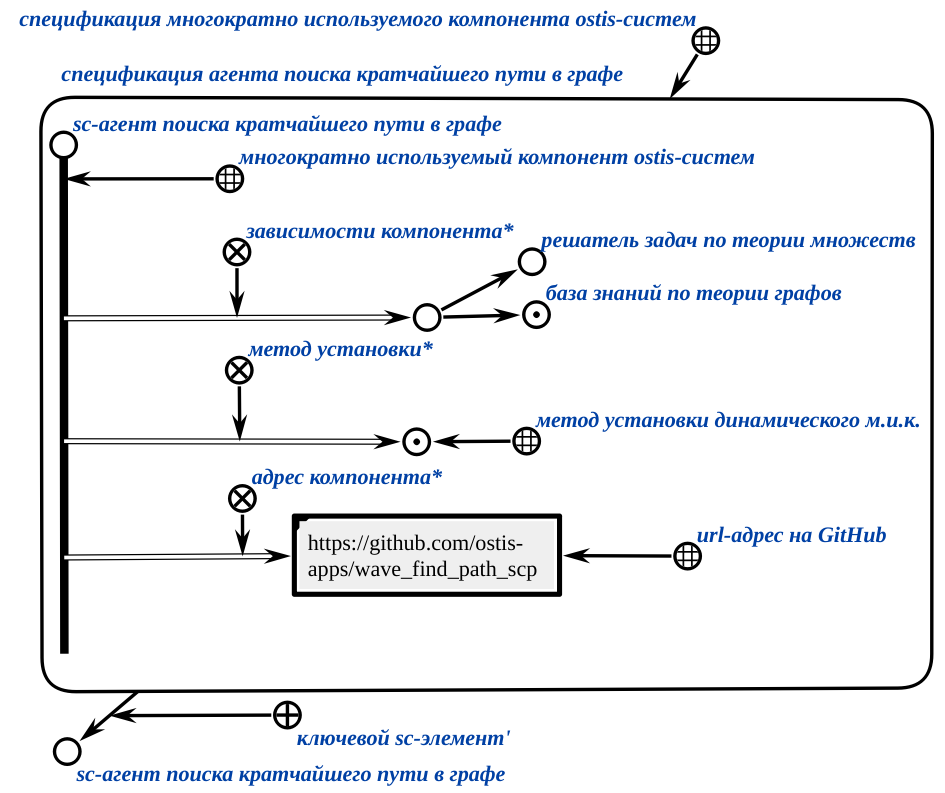
\includegraphics[scale=0.6]{author/part5/figures/component_required_specification_example.png}
	\caption{Пример обязательной части спецификации многократно используемого компонента ostis-систем}
	\label{fig:component_required_specification_example}
\end{figure}

Метод установки позволяет пользователю установить компонент вручную, а \textbf{\textit{менеджеру многократно используемых компонентов ostis-систем}} --- автоматически. Основные два метода установки многократно используемых компонентов --- метод установки \myuline{динамически} устанавливаемого многократно используемого компонента ostis-систем и метод установки многократно используемого компонента, при установке которого система \myuline{требует перезапуска}. При динамической установке необходимо только скачать компонент и, при необходимости, его зависимые компоненты, и он сразу же функционирует в системе. 

\begin{figure}[H]
	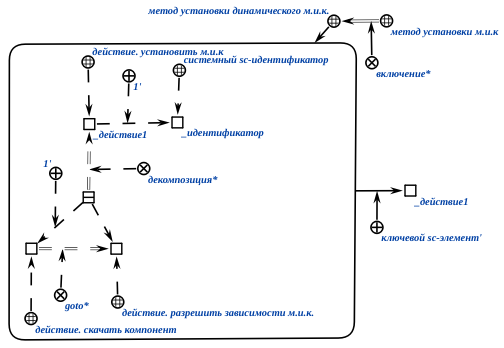
\includegraphics[scale=0.6]{author/part5/figures/install_dynamic_method.png}
	\caption{Метод установки динамически устанавливаемого многократно используемого компонента ostis-систем}
	\label{fig:dynamic_method}
\end{figure}

При установке компонента, при установке которого система требует перезапуска необходимо помимо скачивания компонента транслировать его в память системы.

\begin{figure}[H]
	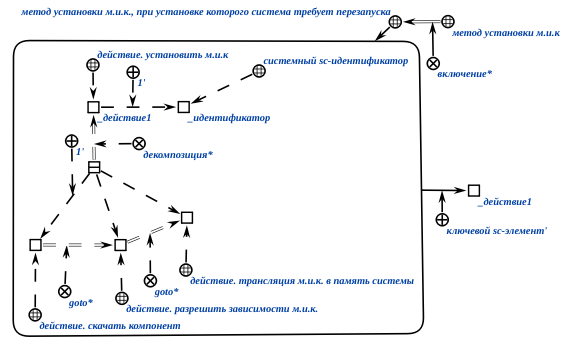
\includegraphics[scale=0.6]{author/part5/figures/install_with_reboot_method.png}
	\caption{Метод установки динамически устанавливаемого многократно используемого компонента, при установке которого система требует перезапуска}
	\label{fig:install_with_reboot_method}
\end{figure}


Связки отношения \textit{адрес хранилища*} связывают многократно используемый компонент, хранящийся в виде внешних файлов и файл, содержащий url-адрес многократно используемого компонента ostis-систем. Таким файлом может быть файл, содержащий url-адрес на GitHub многократно используемого компонента ostis-систем, файл, содержащий url-адрес на Google Drive многократно используемого компонента ostis-систем, файл, содержащий url-адрес на Docker Hub многократно используемого компонента ostis-систем и другие.

Связки отношения \textit{зависимости компонента*} связывают многократно используемый компонент, и множество компонентов, без которых устанавливаемый компонент \myuline{не может быть} встроен в дочернюю ostis-систему.

Спецификация неатомарного многократно используемого компонента должна содержать информацию о том, из каких компонентов он состоит, используя отношение \textit{декомпозиция*}. При этом sc-структура, обозначающая неатомарный компонент не обязана содержать все sc-элементы компонентов, на которые она декомпозируется, достаточно, чтобы неатомарному компоненту принадлежали знаки всех тех компонентов, из которых он состоит (должно быть полное перечисление составных компонентов).

На рисунке \nameref{fig:component_optional_specification_example} изображена необязательная часть спецификации, необходимой для установки sc-агента поиска кратчайшего пути в графе. Полная спецификация компонента является результатом объединения обязательной и необязательной частей. Другие примеры спецификаций многократно используемых компонентов ostis-систем описаны в \textit{\ref{gis_components}~\nameref{gis_components}}.

\begin{figure}[H]
	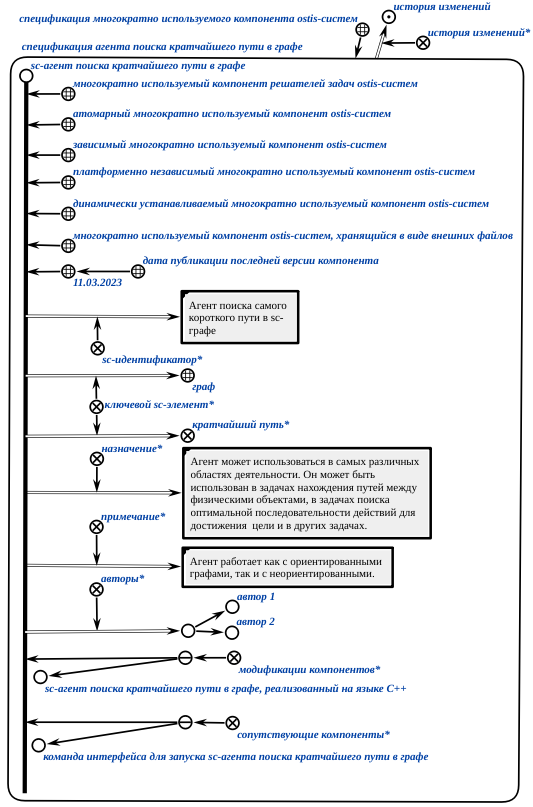
\includegraphics[scale=1.0]{author/part5/figures/component_optional_specification_example.png}
	\caption{Пример необязательной части спецификации многократно используемого компонента ostis-систем}
	\label{fig:component_optional_specification_example}
\end{figure}

В некоторых случаях может оказаться, что для использования одного многократно используемого компонента OSTIS целесообразно или даже необходимо дополнительно использовать несколько других многократно используемых компонентов OSTIS. Например, может оказаться целесообразным вместе с каким либо sc-агентом информационного поиска использовать соответствующую команду интерфейса, которая представлена отдельным компонентом и позволит пользователю задавать вопрос для указанного sc-агента через интерфейс системы. В таких случаях для связи компонентов используется отношение \textit{сопутствующие компоненты*}. Наличие таких связей позволяет устранить возможные проблемы неполноты знаний и навыков в дочерней системе, из-за которых какие-либо из компонентов могут не выполнять свои функции. Связки отношения \textit{сопутствующий компонент*} связывают многократно используемые компоненты ostis-систем, которые целесообразно использовать в дочерней системе вместе. Каждая такая связка может дополнительно быть снабжена sc-комментарием или sc-пояснением, отражающим суть указываемой зависимости. Отношение \textit{история изменений*} позволяет специфицировать различные версии компонента и, при необходимости, устанавливать выбранную пользователем версию. Различные версии, как правило, отражают какие-либо улучшения или исправления ошибок. \textit{Модификации компонентов*} --- это функционально эквивалентные реализации одного и того же компонента, которые могут быть синтаксически эквивалентны (например, реализация одного и того же sc-агента на платформенно-зависимом и пталформенно-независимом уровнях). Развитие Библиотеки OSTIS происходит не только за счёт её пополнения новыми компонентами, но и за счёт появления новых версий и модификаций уже существующих компонентов. Связки отношения \textit{авторы*} связывают многократно используемый компонент со множеством авторов этого компонента. Спецификация может также содержать дополнительную информацию об авторах при необходимости. Отношения \textit{примечание*} и \textit{пояснение*} связывают многократно используемый компонент и некоторый текст (как естественно-языковой, так и текст на языке SC), который является примечанием или пояснением к этому компоненту. Идентификаторы компонента позволяют пользователям и разработчикам обозначать компонент, используя внешний язык. Ключевые sc-элементы компонента позволяют указать на наиболее важные понятия, связанные с описываемым компонентом. Отношение \textit{назначение*} позволяет описать ожидаемый сценарий, выделить рекомендации использования многократно используемого компонента. Требования полноты и безошибочности специфицируют возможные ограничения и ошибки компонента, область его использования.

\section{Менеджер многократно используемых компонентов ostis-систем}
\label{ostis_library_component_manager}

\begin{SCn}
\begin{scnrelfromlist}{ключевое понятие}
	\scnitem{менеджер многократно используемых компонентов ostis-систем}
\end{scnrelfromlist}
\end{SCn}

\bigskip

\begin{SCn}
\begin{scnrelfromlist}{ключевое знание}
	\scnitem{Минимальные функциональные возможности менеджера компонентов}
	\scnitem{Расширенные функциональные возможности менеджера компонентов}
\end{scnrelfromlist}
\end{SCn}

\bigskip

\textit{менеджер многократно используемых компонентов ostis-систем} --- подсистема ostis-системы, с помощью которой происходит взаимодействие с библиотекой компонентов ostis-систем.

\begin{SCn}
\scnheader{менеджер многократно используемых компонентов ostis-систем}
\scnsubset{встраиваемая ostis-система}
\scnidtftext{часто используемый sc-идентификатор}{менеджер многократно используемых компонентов}
\scnidtftext{часто используемый sc-идентификатор}{менеджер компонентов}
\begin{scnrelfromset}{обобщенная декомпозиция}
	\scnitem{база знаний менеджера многократно используемых компонентов ostis-систем}
	\scnitem{решатель задач менеджера многократно используемых компонентов ostis-систем}
	\scnitem{интерфейс менеджера многократно используемых компонентов ostis-систем}
\end{scnrelfromset}
\end{SCn}

База знаний менеджера компонентов содержит все те знания, которые необходимы для установки многократно используемого компонента в дочернюю ostis-систему. К таким знаниям относятся знания о спецификации многократно используемых компонентов, методы установки компонентов, знание о  библиотеках ostis-систем, с которыми происходит взаимодействие, классификация компонентов и другие. Решатель задач менеджера компонентов взаимодействует с библиотекой ostis-систем и позволяет установить и интегрировать многократно используемые компоненты в дочернюю ostis-систему, также выполнять поиск, обновление, публикацию, удаление компонентов и другие операции с ними. Интерфейс менеджера многократно используемых компонентов обеспечивает удобное для пользователя и других систем использование менеджера компонентов.

\textit{решатель задач менеджера многократно используемых компонентов ostis-систем} как минимум должен обеспечивать следующие функциональные возможности:

\begin{SCn}
\scnheader{менеджер многократно используемых компонентов ostis-систем}
\scnrelfrom{минимальные функциональные возможности}{Минимальные функциональные возможности менеджера компонентов}
\begin{scnindent}
\begin{scneqtoset}
	\scnfileitem{\textbf{Поиск многократно используемых компонентов ostis-систем.} Множество возможных критериев поиска соответствует спецификации многократно используемых компонентов. Такими критериями могут быть классы компонента, его авторы, идентификатор, фрагмент примечания, назначение, принадлежность какой-либо предметной области, вид знаний компонента и другие.}
	\scnfileitem{\textbf{Установка многократно используемого компонента ostis-систем.} Установка многократно используемого компонента происходит вне зависимости от типологии, способа установки и местоположения компонента. Необходимое условие для возможности установки многократно используемого компонента --- наличие \textbf{\textit{спецификации многократно используемого компонента ostis-систем}}. Перед установкой многократно используемого компонента в дочернюю систему необходимо установить все зависимые компоненты. Также для платформенно-зависимых компонентов может быть необходимо установить иные зависимости, которые не являются компонентами какой-либо библиотеки ostis-систем. После успешной установки компонента, в базе знаний дочерней системы генерируется информационная конструкция, обозначающая факт установки компонента в систему с помощью отношения \textit{установленные компоненты*}.}
	\scnfileitem{\textbf{Добавление и удаление отслеживаемых менеджером компонентов библиотек.} Менеджер компонентов содержит информацию о множестве источников для установки компонентов, перечень которых можно дополнять. По умолчанию менеджер компонентов отслеживает Библиотеку Метасистемы OSTIS, однако можно создавать и добавлять дополнительные библиотеки ostis-систем.}
\end{scneqtoset}
\end{scnindent}
\end{SCn}

Исходя из указанных минимальных функциональных возможностей \textit{решатель задач менеджера многократно используемых компонентов ostis-систем} представляет собой следующую иерархию абстрактных sc-агентов:

\begin{SCn}
	\scnheader{решатель задач менеджера многократно используемых компонентов ostis-систем}
	\begin{scnrelfromset}{декомпозиция абстрактного sc-агента}
		\scnitem{Абстрактный sc-агент поиска многократно используемых компонентов ostis-систем}
		\scnitem{Абстрактный sc-агент установки многократно используемых компонентов ostis-систем}
		\scnitem{Абстрактный sc-агент управлением отслеживаемых менеджером компонентов библиотек}
		\begin{scnindent}
			\begin{scnrelfromset}{декомпозиция абстрактного sc-агента}
				\scnitem{Абстрактный sc-агент добавления отслеживаемой менеджером компонентов библиотеки}
				\scnitem{Абстрактный sc-агент удаления отслеживаемой менеджером компонентов библиотеки}
			\end{scnrelfromset}
		\end{scnindent}
	\end{scnrelfromset}
\end{SCn}

Используя минимальные функциональные возможности менеджер компонентов может установить компоненты, которые будут расширять его же функционал. Компоненты, реализующие расширенный функционал менеджера компонентов являются частью \textit{Библиотеки OSTIS}. К расширенному функционалу относится:

\begin{SCn}
\scnheader{менеджер многократно используемых компонентов ostis-систем}
\scnrelfrom{расширенные функциональные возможности}{Расширенные функциональные возможности менеджера компонентов}
\begin{scnindent}
	\begin{scneqtoset}
		\scnfileitem{\textbf{Спецификация} многократно используемого компонента ostis-систем. Менеджер компонентов позволяет специфицировать компоненты, входящие в состав библиотеки ostis-систем, а также специфицировать новые создаваемые компоненты, которые будут публиковаться в библиотеку ostis-систем. При этом спецификация может происходить как автоматически, так вручную. Например, менеджер компонентов может обновить спецификацию используемого компонента в соответствии с тем, в какие новые ostis-системы его установили, обновление спецификации авторства компонента при его редактировании в библиотеке ostis-систем, спецификация ошибок, выявленных в процессе эксплуатации компонента и так далее.}
		\scnfileitem{\textbf{Формирование} многократно используемого компонента ostis-систем по шаблону с заданными параметрами. При установке шаблона многократно используемого компонента ostis-систем менеджер компонентов позволяет сформировать по нему конкретный компонент. Для этого пользователю предлагается определить значения всех sc-переменных в шаблоне для формирования конкретного компонента из некоторой предметной области. Например, для формирования многократно используемого компонента базы знаний, представляющего собой семантическую окрестность некоторого отношения (рисунок \nameref{fig:relation_template}), нужно определить значения всех переменных, кроме переменной, являющейся ключевым sc-элементом данной структуры.}
		\scnfileitem{\textbf{Публикация} многократно используемого компонента ostis-систем в библиотеку ostis-систем. При публикации компонента в библиотеку ostis-систем происходит верификация на основе спецификации компонента. Публикация компонента может сопровождаться сборкой неатомарного компонента из существующих атомарных. Также существует возможность обновления версии опубликованного компонента сообществом его разработчиков.}
		\scnfileitem{\textbf{Обновление} установленного многократно используемого компонента ostis-систем.}
		\scnfileitem{\textbf{Удаление} установленного многократно используемого компонента. Как и в случае установки после удаления многократно используемого компонента из ostis-системы в базе знаний системы устанавливается факт удаления компонента. Эта информация является важной частью \myuline{истории эксплуатации} ostis-системы.}
		\scnfileitem{\textbf{Редактирование} многократно используемого компонента в библиотеке ostis-систем.}
		\scnfileitem{\textbf{Сравнение} многократно используемых компонентов ostis-систем.}
	\end{scneqtoset}
\end{scnindent}
\end{SCn}

Для того, чтобы создать новую ostis-систему "с нуля"{}, используя \textit{ostis-платформу} (см. \textit{\ref{sec_interpreter_ostis_platform}~\nameref{sec_interpreter_ostis_platform}}), необходимо установить некоторый \textit{Программный вариант реализации ostis-платформы} (см. Главу \textit\ref{chapter_soft_platform}~\nameref{chapter_soft_platform}}) с помощью сторонних средств. Такими средствами могут быть (1) хранилища исходного кода платформы, например, облачные хранилища, такие как GitHub репозиторий, с соответствующим набором инструкций по установке платформы или (2) средства установки заранее скомпилированной программной реализации платформы, например, средство установки программного обеспечения apt. Далее установка многократно используемых компонентов в ostis-систему (независимо от типа компонентов) осуществляется с помощью менеджера компонентов. При установке платформенно-зависимых компонентов менеджер компонентов должен управлять соответствующими средствами сборки таких компонентов (CMake, Ninja, npm, grunt и другие).

Компонент находится в некотором хранилище --- (1) библиотеке компонентов ostis-систем или (2) в виде файлов на некотором облачном хранилище. В случае, когда компонент хранится в библиотеке, для его установки менеджер компонентов копирует все sc-элементы, которые представляют собой компонент, в дочернюю ostis-систему. В случае, когда компонент хранится в виде файлов на облачном хранилище, менеджер компонентов скачивает файлы компонента и устанавливает их в соответствии со спецификацией. Адреса хранилищ спецификаций компонентов должны храниться в базе знаний менеджера компонентов, чтобы иметь доступ к спецификациям компонентов для их последующего использования (поиска, установки и так далее). На рисунке \nameref{fig:specification_storage_addresses} приведён пример фрагмента базы знаний менеджера компонентов, который описывает то, где хранятся спецификации компонентов, доступных для установки. Такое хранилище представляет собой множество, состоящее из двух множеств: (1) множество адресов спецификаций компонентов и (2) множество адресов спецификаций других хранилищ. Таким образом, образуется древовидная структура в соответствии с иерархией материнских ostis-систем и соответствующих им библиотек.

\begin{figure}[H]
	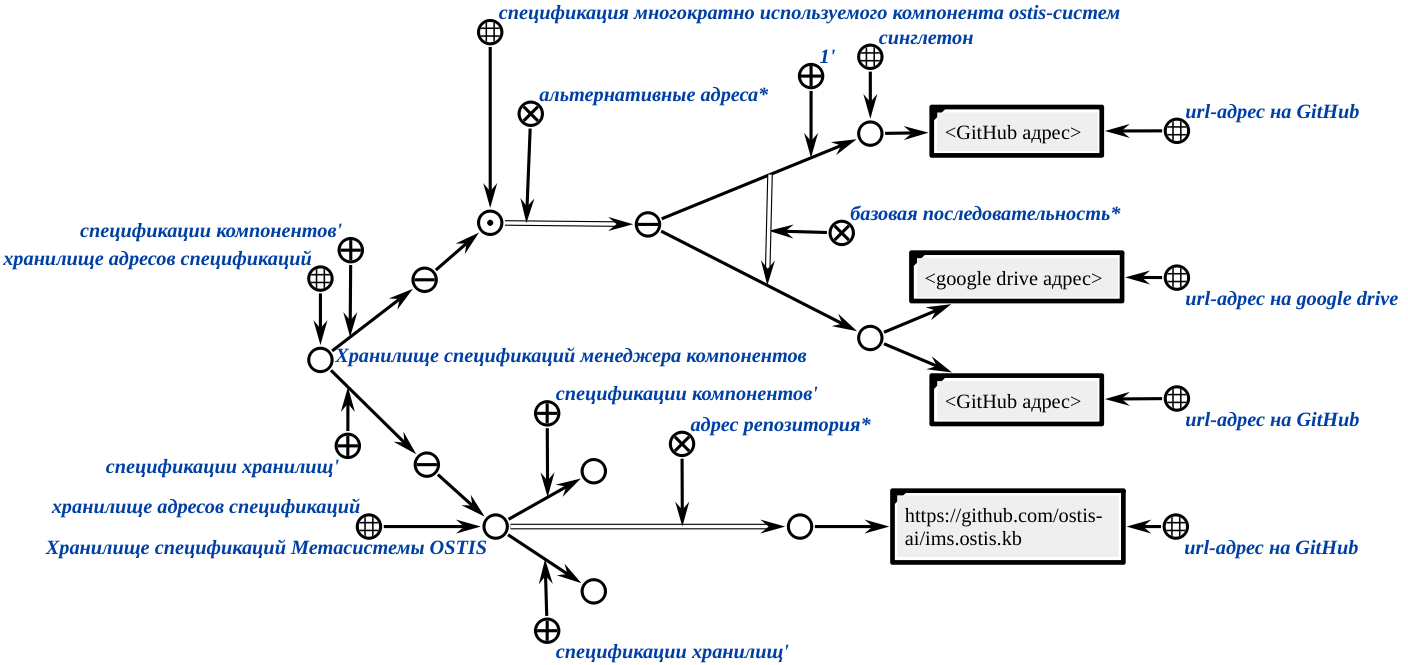
\includegraphics[scale=0.5]{author/part5/figures/specification_storage_addresses.png}
	\caption{Пример структуры хранилища адресов спецификаций компонентов}
	\label{fig:specification_storage_addresses}
\end{figure}

Если указать адрес корня дерева хранилищ адресов спецификаций, то менеджер компонентов получает доступ ко всем спецификациям дочерних хранилищ. При обработке такого дерева спецификаций менеджер компонентов погружает в sc-память спецификации компонентов, доступных для установки, однако не сами эти компоненты.

\textit{менеджер многократно используемых компонентов ostis-систем} является необязательной подсистемой ostis-платформы. Однако система, имеющая менеджер компонентов, может устанавливать компоненты не только сама в себя, но и в другие системы при наличии доступа. Таким образом, одна система может заменить ostis-платформу другой системы, оставив при этом \textit{sc-модель кибернетической системы} (см. \textit{\ref{sec_interpreter_ostis_impl}~\nameref{sec_interpreter_ostis_impl}}). Таким же образом некоторая ostis-система может порождать другие ostis-системы, используя компонентный подход.

Включение компонента в дочернюю ostis-систему в общем случае состоит из следующих этапов:
\begin{textitemize}
	\item поиск подходящего компонента во множестве доступных библиотек;
	\item выделение компонента в виде, удобном для транспортировки в дочернюю ostis-систему с указанием версии и модификации при необходимости (например, выбор доступного хранилища компонента, выбор оптимального варианта реализации компонента с учётом состава дочерней системы);
	\item установка многократно используемого компонента и его зависимостей (с указанием версии и модификации при необходимости);
	\item интеграция компонента в дочернюю систему;
	\item поиск и устранение ошибок и противоречий в дочерней системе.
\end{textitemize}

Данный процесс с точки зрения пользователя не зависит от типа компонента и особенностей его реализации.

\section*{Заключение Главы \ref{chapter_library}}
\label{ostis_library_conclusion}

Компонентный подход является ключевым в технологии проектирования интеллектуальных компьютерных систем. Вместе с этим, технология компонентного проектирования тесно связана с остальными составляющими технологии проектирования интеллектуальных компьютерных систем и обеспечивает их совместимость, производя мощнейший синергетический эффект при использовании всего комплекса частных технологий проектирования интеллектуальных систем. Важнейшим принципом в реализации компонентного подхода является семантическая совместимость многократно используемых компонентов, что позволяет минимизировать участие программистов в создании новых компьютерных систем и в совершенствовании существующих.

Для реализации компонентного подхода в работе предложена библиотека многократно используемых совместимых компонентов интеллектуальных компьютерных систем на основе Технологии OSTIS, введена классификация и спецификация многократно используемых компонентов ostis-систем, предложена модель менеджера компонентов, позволяющего взаимодействовать ostis-системам с библиотеками многократно используемых компонентов и управлять компонентами в системе, рассмотрена архитектура экосистемы интеллектуальных компьютерных систем с точки зрения использования библиотеки многократно используемых компонентов.

Полученные результаты позволят повысить эффективность проектирования интеллектуальных систем и средств автоматизации разработки таких систем, а также обеспечить возможность не только разработчику, но и интеллектуальной системе автоматически дополнять систему новыми знаниями и навыками.

%\input{author/references}
\chapter{Методика и средства проектирования и анализа качества баз знаний ostis-систем}
\chapauthortoc{Бутрин С.В.\\Шункевич Д.В.\\Банцевич К.А.}
\label{chapter_kb_design}

\vspace{-7\baselineskip}

\begin{SCn}
	\begin{scnrelfromlist}{автор}
		\scnitem{Бутрин С.В.}
		\scnitem{Шункевич Д.В.}
		\scnitem{Банцевич К.А.}
	\end{scnrelfromlist}

\bigskip

\scntext{аннотация}{В главе рассматриваются актуальные проблемы текущего состояния средств проектирования и анализа качеств баз знаний, предложен подход к их решению на основе Технологии OSTIS. Сформулированы принципы коллективного проектирования и разработки баз знаний. Сформулированы принципы верификации баз знаний.}

\bigskip

\begin{scnrelfromlist}{подраздел}
	\scnitem{\ref{sec_kb_design_methods}~\nameref{sec_kb_design_methods}}
	\scnitem{\ref{sec_kb_design_individual}~\nameref{sec_kb_design_individual}}	\scnitem{\ref{sec_kb_design_collective}~\nameref{sec_kb_design_collective}}
	\scnitem{\ref{sec_kb_design_contradiction}~\nameref{sec_kb_design_contradiction}}
	\scnitem{\ref{sec_kb_design_hole}~\nameref{sec_kb_design_hole}}
	\scnitem{\ref{sec_kb_design_developers}~\nameref{sec_kb_design_developers}}
	\scnitem{\ref{sc_kb_design_components}~\nameref{sc_kb_design_components}}
\end{scnrelfromlist}

\bigskip

\begin{scnrelfromlist}{ключевое понятие}
	\scnitem{база знаний}
	\scnitem{редактор баз знаний}
	\scnitem{разработка баз знаний}
	\scnitem{разработчик}
	\scnitem{противоречие}
	\scnitem{информационная дыра}
	\scnitem{многократно используемые компоненты}
\end{scnrelfromlist}

\bigskip

\begin{scnrelfromlist}{библиографическая ссылка}
	\scnitem{\scncite{Arshinskiy2020}}
	\scnitem{\scncite{Rybina2007}}
	\scnitem{\scncite{Zhang2023}}
\end{scnrelfromlist}

\end{SCn}

\section*{Введение в Главу \ref{chapter_kb_design}}

\section{Действия и методики проектирования баз знаний ostis-систем}
\label{sec_kb_design_methods}

Проектирование базы знаний включает в себя два аспекта: индивидуальный и коллективный.

Индивидульный представляет собой наполнение изолировнной части базы знаний конкретным пользователем.

Коллективный представляет собой согласование все базы знаний и включает в себя процесс внедрения изменений и внесения предложений.

Таким образом индивидуальный аспект включает в себя средства и методы позволяющие пользователю непосредственно наполнять базу знаний посредствам редакторов, трансляторов и т.д. При этом процесс редактирования базы знаний должен быть максимально удобным и понятным для пользователя.

В идеале редактор должен являться частью системы и должен быть описан в самой базе знаний, так как система имеющая всю информацию о редакторе может позволить пользователю эффективно с ним взаимодействовать засчет системы поддержки. Такая система поддержки должна позволить пользователю непрерывно и (незаметно? естественно?) овладевать редактором учитывая при это особенности как самого редактора (его интерфейса, возможностей и т.д.) , так и самого пользоватлея (его предпочтения, ограничения и т.д.)

Коллективный же процесс включает в себя средства и методы для автоматического или полуавтоматического согласования общей базы знаний с индивидуальными базами знаний пользователей. Т.е. он включает в себя процессы создания предложений по изменнеию, их рассмотрение и внесение в общую базу знаний.

Процесс разработки базы знаний включает в себя следующие стадии:
\begin{textitemize}
	\item Формирование начальной структуры гибридной базы знаний, которая предполагает:
		\begin{textitemize}
			\item  формирование структуры разделов базы знаний, соответствующей варианту структуризации базы знаний с точки зрения разработчиков, описан-ному в подразделе 2.6.3 данной диссертационной работы;
			\item выявление описываемых предметных областей;
			\item построение иерархической системы описываемых предметных областей;
			\item построение иерархии разделов базы знаний в рамках предметной	части базы знаний, учитывающей построенную на предыдущем этапе иерархию предметных областей.
		\end{textitemize}
	\item Выявление компонентов базы знаний, которые могут быть заимствованы из библиотеки многократно используемых компонентов баз знаний, и включение их в состав разрабатываемой базы знаний;
	\item Формирование проектных заданий на разработку недостающих фрагментов базы знаний и распределение заданий между разработчиками;
	\item Разработка и согласование фрагментов базы знаний, которые, в свою	очередь, могут в дальнейшем быть включены в состав библиотеки многократно используемых компонентов баз знаний;
	\item Верификация и отладка базы знаний.
\end{textitemize}

Следует отметить, что в процессе совершенствования базы знаний этапы 3 - 5 выполняются циклически.

Для обеспечения свойства рефлексивности интеллектуальной системы, в частности, возможности автоматизации анализа истории эволюции базы знаний и генерации планов по ее развитию, вся деятельность, связанная с разработкой базы знаний, должна специфицироваться в самой этой базе знаний теми же средствами, что и предметная часть.

\section{Индивидуальный аспект проектирования и разработки баз знаний ostis-систем}
\label{sec_kb_design_individual}

\section{Коллективный аспект проектирования и разработки баз знаний ostis-систем}
\label{sec_kb_design_collective}

Для решения указанной задачи разработана модель деятельности, направленной на создание гибридных баз знаний коллективом разработчиков.

Данная модель базируется на модели деятельности различных субъектов и реализована в виде онтологии предметной области деятельности разработчиков, направленной на разработку и модификациюгибридных баз знаний.

Процесс создания и редактирования базы знаний ostis-системы сводится к формированию разработчиками предложений по редактированию того или иного раздела базы знаний и последующему рассмотрению этих предложений администраторами базы знаний.

Кроме того, предполагается, что в случае необходимости для верификации поступающих предложений по редактированию базы знаний могут привлекаться эксперты, а управление процессом разработки осуществляется менеджерами соответствующих проектов по разработке базы знаний.

При этом формирование проектных заданий и их спецификация осуществляются также при помощи механизма предложений по редактированию соответствующего раздела базы знаний. 

Таким образом, вся информация, связанная с текущими процессами разработки базы знаний, историей и планами ее развития, хранится в той же базе знаний, что и ее предметная часть, т. е. часть базы знаний, доступная конечному пользователю системы. Такой подход обеспечивает широкие возможности автоматизации процесса создания баз знаний, а также последующего анализа и совершенствования базы знаний.

Каждое предложение по редактированию базы знаний представляет собой структуру, содержащую sc-текст, который предлагается включить в состав согласованной части базы знаний. В состав таких предложений могут входить знаки действий по редактированию базы знаний, которые автоматически инициируются и выполняются соответствующими агентами после утверждения предложения.


\section{Логико-семантическая модель ostis-системы обнаружения и анализа ошибок и противоречий в базе знаний ostis-системы}
\label{sec_kb_design_contradiction}

Важным этапом в разработке любой системы является контроль качества, так как именно на этом этапе определяется степень жизнеспособности и эффективности системы.

Верификация является видом анализа качества и часть процесса разработки. Она заключается в проверке информации на правильность и точность.
Ее целью является выявление ошибок, различных дефектов и недоработок для своевременного их устранения.

Cуществующие на данный момент методы верификации хорошо развиты и разработано большое количество различных моделей верификации, использующих расширенные таблицы решения, сети Петри, различные логики, например, логики с векторной семантикой (см. \scncite{Arshinskiy2020}) и другие модели. Более того формируются специализированные онтологии для описания многообразия средств и моделей верификации баз знаний (см. \scncite{Rybina2007}). Однако механизма взаимодействия средств, использующих данные методы, нет.

Поэтому средства верификации баз знаний, существующие на данный момент, обладают рядом таких проблем как (см. \scncite{Zhang2023}):
\begin{textitemize}
    \item зависимость от формата представления информации, из-за чего приходится тратить дополнительно время на конвертирование информацию
    \item проблема невозможности быть переиспользованными, так как средства обычно делаются с учетом особенностей конкретной системы
    \item проблема отсутствия механизма взаимодействия средств верификации и анализа знаний
    \item высокая роль человека в процессе верификации, так как самым распространенным способом верификации баз знаний является ручная проверка базы экспертом, человек выступает как администратор, принимающий единогласное решение, навязывая свое мнение системе
    \item современные средства не учитывают и не рассматривают процесс верификации в рамках взаимодействия систем друг с другом.
\end{textitemize}

Эти проблемы могли бы быть решены, если:
\begin{textitemize}
    \item использовать унифицированный и удобный формат представления знаний
    \item системы создавались бы по общей методологии и были бы совместимы друг с другом
    \item продумать и реализовать механизм позволяющий системе стремиться самой принимать решение относительно своего состояния и наличия в нем проблемных моментов и ошибок, система может допускать ошибки и не всегда принимать верные решения, но это должны быть ее ошибки, а не экспертов и разработчиков
\end{textitemize}

Преимуществами Технологии OSTIS в рамках задачи верификации являются:
\begin{textitemize}
    \item наличие общей методологии проектирования интеллектуальных систем, позволяющая решить проблему совместимости систем при их коллективном взаимодействии;
    \item все знания представлены в унифицированном виде, что позволяет эффективно их обрабатывать, сводя затраты на конвертирование к минимуму;
   \item средства, с помощью которых производится выявление, анализ и устранение противоречий описаны в самой базе знаний, а так же их спецификация представлены в самой базе знаний системы, тем самым обеспечивая легкость их расширения и позволяя системе знать, каким инструментарием она обладает;
   \item отсутствие семантических эквивалентных фрагментов, что обеспечивает локальность вносимых исправлений и исключает необходимость вносить исправления многократно в разных местах;
   \item многоагентный подход, который позволяет рассматривать средства анализа и верификации баз знаний как коллектив агентов, способных взаимодействовать друг с другом и дальнейшем принимать общее решение касательно состояния базы знаний. 
\end{textitemize}

Предлагаемый подход сводится к разработке:
\begin{textitemize}
    \item специализированной \textit{предметной области и онтологии}, которая бы содержала бы в себе все необходимые знания о возможных видах проблемных фрагментов базы знаний и способах их исправления
    \item алгоритма, позволяющего системе выявить в себе проблемные фрагменты и устранить их, при этом обеспечив согласованность работы средств самой системы
    \item специализированного решателя задач, содержащего необходимые агенты для выявления и устранения проблемных фрагментов
\end{textitemize}

%% ССылки и объяснение что есть что
Качество базы знаний во многом определяется уровнем наличия/отсутствия не-факторов (см. \scncite{Narinjani2004}) в базе знаний.
\begin{SCn}
\scnheader{не-фактор}
\scnidtf{группа семантических свойств, определяющих качество информации, хранимой в памяти кибернетической системы}
\begin{scneqtoset}
 \scnitem{корректность/некорректность информации, хранимой в памяти кибернетической системы}
 \scnitem{однозначность/неоднозначность информации, хранимой в памяти кибернетической системы}
 \scnitem{целостность/нецелостность информации, хранимой в памяти кибернетической системы}
 \scnitem{чистота/загрязненность информации, хранимой в памяти кибернетической системы}
 \scnitem{достоверность/недостоверность информации, хранимой в памяти кибернетической системы}
 \scnitem{точность/неточность информации, хранимой в памяти кибернетической системы}
 \scnitem{четкость/нечеткость информации, хранимой в памяти кибернетической системы}
 \scnitem{определенность/недоопределенность информации, хранимой в памяти кибернетической системы}
\end{scneqtoset}
\end{SCn}

%\begin{SCn}
%\scnheader{непротиворечивость/противоречивость информации, хранимой в памяти кибернетической системы}
%\scnidtf{уровень присутствия в хранимой информации различного вида противоречий и, в частности, ошибок}

%\scnheader{противоречие*}
%\scnidtf{пара противоречащих друг другу фрагментов информации, хранимой в памяти кибернетической системы*}
%\scntext{примечание}{Чаще всего противоречащими друг другу информационными фрагментами являются:
	%\begin{scnitemize}
	%\item явно представленная в памяти некоторая закономерность (некоторое правило)
	%\item информационный фрагмент, не соответствующий (противоречащий) указанной закономерности
	%\end{scnitemize}}
	
	%\scnheader{полнота/неполнота информации, хранимой в памяти кибернетической системы}
	%\scnidtf{уровень того, насколько информация, хранимая в памяти кибернетической системы, описывает среду существования этой системы и используемые ею методы решения задач достаточно полно (достаточно детально) для того, чтобы кибернетическая система могла действительно решать все множество соответствующих ей задач}
	
	%\scnheader{чистота/загрязненность информации, хранимой в памяти кибернетической системы}
	%\scnidtf{многообразие форм и общее количество информационного мусора, входящего в состав информации, хранимой в памяти кибернетической системы}
	%\end{SCn}


%% Описать что это такое и зачем выделяется
\begin{SCn}
\scnheader{проблемная структура}
\scnidtf{структура, описывающая проблемный фрагмент базы знаний}
\scnidtf{структура, описывающая некачественный фрагмент базы знаний}
\begin{scnreltoset}{объединение}
\scnitem{некорректная структура}
\begin{scnindent}
	\scnidtf{структура, содержащая фрагменты, противоречащие каким либо правилам или закономерностям описанным в базе знаний}
\end{scnindent}
\scnitem{структура, описывающая неполноту в базе знаний}
\begin{scnindent}
	\scnidtf{структура, в которой имеется неполнота (то есть имеется некоторое количество информационных дыр)}
	\scntext{примечание}{Под структурой, описывающей неполноту в базе знаний, понимается структура, содержащая фрагмент базы знаний, в котором отсутствует какая-либо информация, которая необходима (или, по крайней мере, желательна) для однозначного и полного понимания смысла данного фрагмента.}
	%% Переформулировать
\end{scnindent}
\scnitem{информационный мусор}
\begin{scnindent}
	\scnidtf{структура, удаление которой существенно не усложнит деятельность системы}
	\scnidtf{структура, содержащая фрагмент базы знаний, который по каким-либо причинам стал ненужным и требует удаления}
\end{scnindent}
\end{scnreltoset}
\end{SCn}
% Больше про определение противоречия, уточнить что чему противоречит 
\begin{SCn}
\scnheader{противоречие*}
\scnidtf{пара противоречащих друг другу фрагментов информации, хранимой в памяти кибернетической системы*}
\scntext{примечание}{Чаще всего противоречащими друг другу информационными фрагментами являются:
	\begin{scnitemize}
		\item явно представленная в памяти некоторая закономерность (некоторое правило)
		\item информационный фрагмент, не соответствующий (противоречащий) указанной закономерности
	\end{scnitemize}
	В этом случае некорректность может присутствовать:
	\begin{scnitemize}
		\item либо в информационном фрагменте, который противоречит указанной закономерности;
		\item либо в самой этой закономерности;
		\item либо и там и там.
	\end{scnitemize}
		%% Переформулировать
}
\end{SCn}
	
\begin{SCn}
\scnheader{некорректная структура}
\begin{scnreltoset}{включение}
	\scnitem{дублирование системных идентификаторов}
	\scnitem{несоответствие элементов связки доменам отношения}
	\scnitem{цикл по отношению порядка}
	\scnitem{структура, противоречащая свойству единственности}
\end{scnreltoset}
	
\scnheader{структура, описывающая неполноту в базе знаний}
\begin{scnreltoset}{включение}
	\scnitem{не указан максимальный класс объектов исследования предметной области}
	\scnitem{для сущности указан системный, но не указаны основные идентификаторы для всех внешних языков}
	\scnitem{не указаны домены отношения}
	\scnitem{понятие не соотнесено ни с одной предметной областью}
\end{scnreltoset}
\end{SCn}

%% Больше описать, привести примеры, вообщем пересмотреть

\begin{SCn}
\scnheader{требующее внимание разработчика}
\scnidtf{проблемная структура, для исправления которой требуется участие разработчика}
\scnheader{множество элементов, которые должны быть удалены для исправления структуры*}
\scnidtf{множество элементов, удаление которых из структуры позволяет устранить в ней противоречие}
\scnheader{множество элементов, которые должны быть добавлены для исправления структуры*}
\scnidtf{множество элементов, добавление которых в структуру позволяет устранить в ней противоречия}
\scnheader{структура, которую система не способна исправить сама}
\scnidtf{структура, в которой система не способна автоматически устранить противоречия}
%% Возможно переформулировать на что-нибудь покороче


\scnheader{следует отличать*}
\begin{scnhaselementset}
\scnitem{структура, которая система не может решить сама}
\begin{scnindent}
	\scntext{примечание}{Здесь структура, которую система не может решить сама, не может быть исправлена при взаимодействии с разработчиком и требует полного исправления от самого разработчика}
\end{scnindent}
\scnitem{требующее внимание разработчика}
\begin{scnindent}
	\scntext{примечание}{Здесь структура, требующая внимания разработчика, может быть решена в процессе верификации, но потребуется участие разработчика}
\end{scnindent}
\end{scnhaselementset}

%% Описать идею мезанизма согласования средств верификации

\scnheader{Решатель задач средств выявления и устранения противоречий}
\begin{scnreltoset}{декомпозиция абстрактного sc-агента}
\scnitem{Неатомарный агент выявления противоречий}
	\begin{scnindent}
		\scnidtf{Множество агентов, обеспечивающих поиск и фиксирование противоречий в структуре}
	\end{scnindent}
\scnitem{Неатомарный агент устранения противоречий}
	\begin{scnindent}
	\scnidtf{Множество агентов, создающих предложения по исправлению противоречий}
	\scntext{примечание}{Результатом работы таких агентов будут множества предлагаемых к удалению из структуры или добавлению в структуру элементов}
	\end{scnindent}
\scnitem{Агент слияния структур}
	\begin{scnindent}
	\scnidtf{Агент, создающий структуру содержащую все элементы сливаемых структур}
	\end{scnindent}
\scnitem{Агент применения предложений по устранению противоречий}
\scnitem{Агент внесения исправлений в базу знаний}
	\begin{scnindent}
	\scntext{примечание}{Внесение изменений подразумевает не только исправление в базе знаний изначальной проблемной структуры, но и фиксацию самого факта изменения состояния базы знаний}.
	\end{scnindent}
\scnitem{Неатомарный агент верификации структуры}
	\begin{scnindent}
	\scntext{примечание}{Агент обеспечивающий полный цикл верификации структуры координирую другие агенты}
	\end{scnindent}
\end{scnreltoset}
\end{SCn}
%% Добавить про алгоритм

%% Не ограничиваться средствами верификации, затронуть механизмы предотвращения проблемных ситуаций 

%% Рассмотреть верификацию в рамках взаимодействия систем


\section{Логико-семантическая модель ostis-системы обнаружения и анализа информационных дыр в базе знаний ostis-системы} 
\label{sec_kb_design_hole}
Нужно согласовать и возможно объеденить в раздел выше

\section{Логико-семантическая модель ostis-системы автоматизации управления взаимодействием разработчиков различных категорий в процессе проектирования базы знаний ostis-системы}
\label{sec_kb_design_developers}

\begin{SCn}
\scnheader{пользователь базы знаний ostis-системы*}
\scnidtf{бинарное отношение, связывающее sc-модель базы знаний ostis-системы и sc-элемент, обозначающий персону, участвующую в разработке или эксплуатации этой базы знаний}
\scniselement{бинарное отношение}
\scniselement{ориентированное отношение}
\scnnote{Данное отношение отражает связь пользователя и базы знаний в целом, при этом тот же сам пользователь может быть связан другими более частными отношениями с какими-либо фрагментами этой же базы знаний.}

\scnrelfrom{разбиение}{\scnkeyword{Типология отношений между базами знаний ostis-систем и их пользователями по наличию факта прохождения регистрации в этих ostis-системах\scnsupergroupsign}}
\begin{scnindent}
	\begin{scneqtoset}
		\scnitem{зарегистрированный пользователь*}
		\scnitem{незарегистрированный пользователь*}
	\end{scneqtoset}
\end{scnindent}


\end{SCn}


%% Описать механизм редактирования, сравнение с аналогами, акцент на описание стадий с учетом каждой роли 
\begin{SCn}
\scnheader{пользователь, обладающий правом просмотра sc-структуры*}
\scnidtf{бинарное отношение, связывающее sc-элемент, обозначающий sc-структуру (например, фрагмент sc-модели базы знаний), и sc-элемент, обозначающий пользователя этой ostis-системы, который обладает правом просмотра этой sc-структуры.}
\scniselement{бинарное отношение}
\scniselement{ориентированное отношение}
\scntext{примечание*}{Пользователь, обладающий правом просмотра sc-структуры базы знаний ostis-системы может быть зарегистрирован или не зарегистрирован в sc-модели базы знаний.}

\scnheader{пользователь, обладающий правом редактирования sc-структуры*}
\scnidtf{бинарное отношение, связывающее sc-элемент, обозначающий sc-структуру (например, фрагмент sc-модели базы знаний), и sc-элемент, обозначающий зарегистрированного пользователя ostis-системы, который обладает правом редактирования этой sc-структуры.}
\scniselement{бинарное отношение}
\scniselement{ориентированное отношение}
\scnsuperset{пользователь, обладающий правом просмотра sc-структуры*}
\scntext{пояснение}{Связки отношения пользователя, обладающий правом редактирования sc-структуры ostis-системы* связывают sc-структуру (не обязательно всю sc-модель базы знаний) и пользователя, зарегистрированного в этой sc-модели базы знаний.}
\begin{scnrelfromset}{покрытие}
	\scnitem{пользователь, обладающий правом редактирования sc-структуры посредством формирования предложений по внесению изменений в согласованную часть базы знаний этой ostis-системы*}
	\scnitem{пользователь, обладающий правом редактирования sc-структуры с автоматическим формированием и принятием предложений по внесению изменений в согласованную часть базы знаний этой ostis-системы*}
\end{scnrelfromset}

\scnheader{разработчик*}
\scnsubset{пользователь, обладающий правом редактирования sc-структуры*}
\scnidtf{бинарное отношение, связывающее sc-элемент, обозначающий некоторый раздел базы знаний (в пределе – всю базы знаний), и sc-элемент, обозначающий пользователя ostis-системы, который может быть разработчиком данного раздела базы знаний, т. е. выполнять проектные задачи в рамках данного раздела}

\scnrelfrom{разбиение}{\scnkeyword{Типология разработчиков баз знаний ostis-систем\scnsupergroupsign}}
\begin{scnindent}
	\begin{scneqtoset}
		\scnitem{администратор*}
		\scnitem{менеджер*}
		\scnitem{эксперт*}
	\end{scneqtoset}
\end{scnindent}

%\scnheader{администратор*}
%:= [бинарное отношение, связывающее sc-элемент, обозначающий некоторый раздел базы знаний (в пределе – всю базы знаний), и sc-элемент, обозначающий пользователя ostis-системы, который является администратором данного раздела базы знаний]
%
%=> функции*:
%{
%	[контроль целостности и непротиворечивости всей базы знаний]
%	[определение уровней доступа других пользователей]
%	[принятие решения относительно принятия или отклонения предложений в различные части базы знаний, в том числе при необходимости отправка их на экспертизу]
%	[самостоятельное внесение изменений в различные части базы знаний путем использования соответствующих команд редактирования (при этом изменения автоматически оформляются как предложения и заносятся в раздел истории развития ostis-системы)]
%}
%
%
%менеджер*
%:= [бинарное отношение, связывающее sc-элемент, обозначающий некоторый раздел базы знаний (в пределе – всю базы знаний), и sc-элемент, обозначающий персону, которая является менеджером данного раздела базы знаний]
%
%=> функции*:
%{
%	[планирование объемов работ по разработке базы знаний]
%	[детализация проектных задач на подзадачи, непосредственно формулирование проектных задач, назначение исполнителей проектных задач]
%	[установка приоритетов и сроков выполнения задач]
%	[контроль сроков выполнения проектных задач]
%}
%
%эксперт*
%:= [бинарное отношение, связывающее sc-элемент, обозначающий какой-либо проект по разработке раздела базы знаний ostis-системы (в общем случае - всей базы знаний), и sc-элемент, обозначающий персону, которая является экспертом данного раздела базы знаний
%
%=> функции*:
%{
%	[верификация результатов выполнения проектных задач]
%	[при необходимости эксперт может оставлять комментарии к любому фрагменту базы знаний относительно его корректности. Все комментарии попадают в раздел, описывающий план развития компьютерной системы]
%}


\end{SCn}

\section{Многократно используемые компоненты баз знаний ostis-систем}
\label{sc_kb_design_components}

На сегодняшний день разработано большое число \textit{баз знаний} по самым различным предметным областям. Однако в большинстве случаев каждая база знаний разрабатывается отдельно и независимо от других, в отсутствие единой унифицированной формальной основы для представления знаний, а также единых принципов формирования систем понятий для описываемой предметной области. В связи с этим разработанные базы оказываются, как правило, несовместимы между собой и не пригодны для повторного использования. Компонентный подход к разработке интеллектуальных компьютерных систем, реализуемый в виде \textbf{\textit{библиотеки многократно используемых компонентов ostis-систем}}, позволяет решить описанные проблемы.

%\input{author/references}
\chapter{Методика и средства компонентного проектирования решателей задач ostis-систем}
\chapauthortoc{Шункевич Д.В.\\Марковец В.С.}
\label{chapter_ps_design}

\vspace{-7\baselineskip}

\begin{SCn}

\begin{scnrelfromlist}{автор}
	\scnitem{Шункевич Д.~В.}
	\scnitem{Марковец В.~С.}	
\end{scnrelfromlist}

\bigskip

\abstract{В главе рассматривается методика построения и модификации \textit{решателей задач} \textit{ostis-систем}, модель системы автоматизации проектирования \textit{решателей задач}, а также принципы организации \textit{библиотеки многократно используемых компонентов решателей задач ostis-систем}.}

\bigskip

\begin{scnrelfromlist}{подраздел}
    \scnitem{\ref{sec_ps_design_methodology}~\nameref{sec_ps_design_methodology}}
    \scnitem{\ref{sec_auto_sys_for_des_ps}~\nameref{sec_auto_sys_for_des_ps}}
    \scnitem{\ref{sec_ps_components}~\nameref{sec_ps_components}}
\end{scnrelfromlist}

\bigskip

\begin{scnrelfromlist}{ключевой знак}
	\scnitem{Методика построения и модификации машины обработки знаний ostis-систем}
	\scnitem{Система автоматизации проектирования решателей задач ostis-систем}
\end{scnrelfromlist}

\bigskip

\begin{scnrelfromlist}{ключевое понятие}
    \scnitem{решатель задач ostis-системы}
%    \scnitem{sc-агент}
%    \scnitem{scp-программа}
%    \scnitem{база знаний}
%    \scnitem{точка останова*}
    \scnitem{точка останова}
%    \scnitem{некорректность в scp-программе*}
    \scnitem{некорректность в scp-программе}
    \scnitem{ошибка в scp-программе}
%    \scnitem{Метасистема OSTIS}
%    \scnitem{библиотека многократно используемых компонентов ostis-систем}
%    \scnitem{Решатель задач системы автоматизации проектирования агентов обработки знаний}
%    \scnitem{Решатель задач системы автоматизации проектирования scp-программ}
%    \scnitem{команда пользовательского интерфейса системы автоматизации проектирования решателей задач ostis-систем}
%    \scnitem{команда пользовательского интерфейса системы автоматизации проектирования агентов обработки знаний}
%    \scnitem{команда пользовательского интерфейса системы автоматизации проектирования scp-программ}
%    \scnitem{библиотека многократно используемых компонентов решателей задач}
    \scnitem{многократно используемый компонент решателей задач}
%    \scnitem{метод}
%    \scnitem{Средства автоматизации библиотеки многократно используемых компонентов решателей задач}
%    \scnitem{отношение, специфицирующее многократно используемый компонент решателей задач ostis-систем}
%    \scnitem{Решатель задач библиотеки многократно используемых компонентов решателей задач}
\end{scnrelfromlist}

\bigskip

\begin{scnrelfromlist}{библиографическая ссылка}
	\scnitem{\scncite{Shunkevich2013}}
	\scnitem{\scncite{Shunkevich2015}}
	\scnitem{\scncite{Shunkevich2015a}}
	\scnitem{\scncite{Golenkov2015}}
	\scnitem{\scncite{Shunkevich2018}}
	\scnitem{\scncite{Borisov2014}}
	\scnitem{\scncite{Gribova2015a}}
\end{scnrelfromlist}
\end{SCn}

\section*{Введение в Главу \ref{chapter_ps_design}}

В области разработки \textit{решателей задач} существует большое количество конкретных реализаций, однако вопросы совместимости различных решателей задачи и их компонентов практически не рассматриваются. Гипотетически возможно существование универсального решателя задач, объединяющего в себе все известные способы и методы решения задач. Однако использование такого решателя в прикладных целях не является целесообразным. Таким образом, наиболее приемлемым вариантом становится создание библиотеки совместимых между собой компонентов (см. \textit{\ref{ostis_library_section}~\nameref{ostis_library_section}}), из которых впоследствии может быть собран решатель, удовлетворяющий необходимым требованиям.

Как показано в \textit{Главе \ref{chapter_situation_management} \nameref{chapter_situation_management}}, \textit{решатель задач ostis-системы} представляет собой иерархическую систему \textit{навыков}, которыми владеет ostis-система на текущий момент. В свою очередь, \textit{навык} представляет собой некоторый \textit{метод} решения задач заданного класса и соответствующую ему систему \textit{sc-агентов} (\textit{машину обработки знаний} частного вида), обеспечивающих интерпретацию данного метода. В связи с этим методика проектирования решателей задач ostis-систем фактически сводится к методике проектирования баз знаний ostis-систем (см. \textit{Главу \ref{chapter_kb_design}~\nameref{chapter_kb_design}}) и методике проектирования машин обработки знаний ostis-систем, которая детально рассматривается в данной главе.

Вопросам разработки \textit{решателей задач ostis-систем} посвящен ряд работ, таких как 
\scncite{Shunkevich2013}, \scncite{Shunkevich2015}, \scncite{Golenkov2015}, \scncite{Shunkevich2015a}, \scncite{Shunkevich2018}. Среди других известных работ, посвященных вопросам компонентного проектирования решателей задач в целом, стоит отметить работы \scncite{Borisov2014}, \scncite{Gribova2015a}, в которых, однако, не уделяется внимание разработке комплексной методики проектирования решателей задач, которой посвящена данная глава.

\section{Действия и методики проектирования решателей задач ostis-систем}
\label{sec_ps_design_methodology}
\begin{SCn}
\bigskip

\begin{scnrelfromlist}{ключевой знак}
	\scnitem{Методика построения и модификации машины обработки знаний ostis-систем}
\end{scnrelfromlist}

\bigskip

\begin{scnrelfromlist}{ключевое понятие}
    \scnitem{решатель задач ostis-системы}
    \scnitem{sc-агент}
    \scnitem{scp-программа}
\end{scnrelfromlist}

\end{SCn}

Основу любого решателя задач составляет система sc-агентов, то есть \textit{машина обработки знаний ostis-системы}, в связи с этим целесообразно рассмотреть более детально процесс проектирования \textit{машин обработки знаний ostis-систем}. Приведенная методика разработана с учетом того, что каждая \textit{машина обработки знаний ostis-систем} представляет собой иерархический коллектив sc-агентов.

Построение же общей методики проектирования решателей задач ostis-систем требует также уточнения принципов разработки \textit{методов} решения задач, которые, в свою очередь, тесно пересекаются с общими принципами разработки баз знаний ostis-систем (см. \textit{Главу \ref{chapter_kb_design} \nameref{chapter_kb_design}}). Рассмотрим более подробно \textit{Методику построения и модификации машин обработки знаний ostis-систем}.

\textit{Методика построения и модификации машин обработки знаний ostis-систем} включает несколько этапов:
\begin{textitemize}
    \item формирование требований к машине обработки знаний и ее формальная спецификация;
    \item формирование коллектива sc-агентов, входящих в состав разрабатываемой машины;
    \item разработка алгоритмов атомарных sc-агентов;
    \item реализация программ sc-агентов;
    \item верификация разработанных компонентов;
    \item отладка разработанных компонентов, исправление ошибок.
\end{textitemize}

Предлагаемая методика может быть применена как при разработке \textit{машины обработки знаний} объединенных \textit{решателей задач}, так и при разработке м\textit{ашины обработки знаний} \textit{решателей задач} частного вида, поскольку с формальной точки зрения все такие машины трактуются как \textit{неатомарные абстрактные sc-агенты}.

\textbf{Этап 1. Формирование требований к машине обработки знаний и ее формальная спецификация}

На данном этапе необходимо:
\begin{textitemize}
\item четко выделить задачи, решение которых должен обеспечивать \textit{решатель задач};
\item продумать предполагаемые способы их решения и на основе данного анализа определить место будущей машины обработки знаний \textit{решателя задач} в общей иерархии \textit{решателей задач}.
\end{textitemize}

Важность данного этапа заключается в том, что при правильной классификации существует вероятность того, что в составе \textit{библиотеки многократно используемых компонентов решателей задач ostis-систем} уже есть реализованный вариант требуемой машины обработки знаний. В противном случае, у разработчика появляется возможность включить разработанную машину в \textit{библиотеку многократно используемых компонентов решателей задач ostis-систем} для последующего использования. Данные факты обусловлены тем, что структура \textit{библиотеки многократно используемых компонентов решателей задач ostis-систем} основана на семантической классификации \textit{решателей задач} и, соответственно, их компонентов.

При недостаточно четкой спецификации и классификации разрабатываемого \textit{решателя задач} повышается вероятность того, что подходящая машина обработки знаний не будет найдена в библиотеке компонентов даже в случае, если она там есть, а вновь разработанный \textit{решатель задач} не сможет быть включен в библиотеку. Таким образом, принцип многократного использования уже разработанных компонентов будет нарушен, что существенно повысит затраты на разработку.

\textbf{Этап 2. Формирование коллектива sc-агентов, входящих в состав разрабатываемой машины обработки знаний}

В случае, когда найти в библиотеке готовую машину обработки знаний, удовлетворяющую всем предъявляемым требованиям, не удалось, необходимо выделить (то есть собственно определить множество требуемых компонентов) и специфицировать все ее компоненты.

Результатом данного этапа является перечень полностью специфицированных \textit{абстрактных sc-агентов}, которые войдут в состав разрабатываемой машины обработки знаний, с их иерархией вплоть до \textit{атомарных абстрактных sc-агентов}. В рамках данного этапа очень важно проектировать коллектив агентов таким образом, чтобы максимально задействовать уже имеющиеся в библиотеке многократно используемые компоненты ostis-систем, а при отсутствии нужного компонента --- иметь возможность включить его в библиотеку после реализации.

При разработке перечня sc-агентов (в том числе их спецификаций) необходимо соблюдать ряд принципов:

\begin{textitemize}
\item каждый разрабатываемый sc-агент должен быть, по возможности, предметно независим, то есть во множество ключевых узлов данного sc-агента не должны входить понятия, имеющие отношение непосредственно к рассматриваемой предметной области. Исключение составляют понятия из общих предметных областей, которые носят междисциплинарный характер (например, отношение \textit{включение*} или понятие \textit{действие}, см. \textit{Главу \ref{chapter_top_ontologies} \nameref{chapter_top_ontologies}}). Данное правило также может быть нарушено в случае, если sc-агент является вспомогательным и ориентирован на обработку какого-либо конкретного класса объектов (например, sc-агенты, выполняющие арифметические вычисления, могут напрямую работать с конкретными отношениями \textit{сложение*} и \textit{умножение*} и т. п.). Всю необходимую для решения задачи информацию sc-агент должен извлекать из семантической окрестности соответствующего инициированного действия. Разработанный с учетом указанных требований sc-агент может быть использован при проектировании большего числа ostis-систем, чем в случае, если бы он был реализован с ориентацией на конкретную предметную область. После завершения разработки и отладки такой sc-агент должен быть включен в \textit{библиотеку многократно используемых абстрактных sc-агентов}, которая входит в состав \textit{библиотеки многократно используемых компонентов решателей задач ostis-систем};
\item не стоит путать понятия sc-агент и \textit{агентная программа} (в том числе \textit{агентная scp-программа}). Взаимодействие sc-агентов осуществляется исключительно посредством спецификации информационных процессов в общей памяти, каждый sc-агент реагирует на некоторый класс событий в sc-памяти. Таким образом, каждому sc-агенту соответствует некоторое условие инициирования и одна агентная программа, которая запускается автоматически при возникновении в sc-памяти соответствующего условия инициирования. При этом в рамках данной программы могут сколько угодно раз вызываться различные подпрограммы. Однако не стоит путать инициирование sc-агента, которое осуществляется при появлении в sc-памяти соответствующей конструкции, и вызов подпрограммы другой программой, который предполагает явное указание вызываемой подпрограммы и перечня ее параметров;
\item каждый sc-агент должен самостоятельно проверять полноту соответствия своего условия инициирования текущему состоянию sc-памяти. В процессе решения какой-либо задачи может возникнуть ситуация, когда на появление одной и той же структуры среагировали несколько sc-агентов. В таком случае выполнение продолжают только те из них, условие инициирования которых полностью соответствует сложившейся ситуации. Остальные sc-агенты в данном случае прекращают выполнение и возвращаются в режим ожидания. Выполнение данного принципа достигается за счет тщательного уточнения спецификаций разрабатываемых sc-агентов. В общем случае условия инициирования у нескольких sc-агентов могут совпадать, например, в случае, когда одна и та же задача может быть решена разными способами и заранее неизвестно, какой из них приведет к желаемому результату;
% нужен наглядный пример
\item необходимо помнить, что неатомарный sc-агент с точки зрения других sc-агентов, не входящих в его состав, должен функционировать как целостный sc-агент (выполнять логически атомарные действия), что накладывает определенные требования на спецификации атомарных sc-агентов, входящих в его состав: как минимум, необходимо, чтобы в составе неатомарного sc-агента присутствовал хотя бы один атомарный sc-агент, условие инициирования которого полностью совпадает с условием инициирования данного неатомарного sc-агента;
\item при необходимости реализации нового sc-агента следует руководствоваться следующими принципами выделения атомарных абстрактных \textit{sc-агентов}:

\begin{textitemize}
    \item проектируемый sc-агент должен быть максимально независим от предметной области, что позволит в дальнейшем использовать его при разработке \textit{решателей задач} максимально возможного числа ostis-систем. При этом универсальность предполагает не только минимизацию числа ключевых узлов sc-агента, но и выделение класса действий, выполняемых данным sc-агентом таким образом, чтобы имело смысл включить данный sc-агент в \textit{библиотеку многократно используемых абстрактных sc-агентов} и использовать его при разработке \textit{решателей задач} других ostis-систем. Не следует искусственно увязывать ряд действий в один sc-агент и, наоборот, расчленять одно самодостаточное действие на поддействия: это вызовет сложности восприятия принципов работы sc-агента разработчиками и не позволит использовать sc-агент в ряде систем (например, в обучающих системах, которые должны объяснять ход решения пользователю, см. \textit{Главу \ref{chapter_learning_systems} \nameref{chapter_learning_systems}});
    \item выполняемое данным sc-агентом действие должно быть логически целостным и завершенным. Следует помнить, что все sc-агенты взаимодействуют исключительно через общую sc-память, и избегать ситуаций, в которых инициирование одного sc-агента осуществляется путем явной генерации известного условия инициирования другим \textit{sc-агентом} (то есть, по сути, явным непосредственным вызовом одного sc-агента другим);
    \item имеет смысл выделять в отдельные sc-агенты относительно крупные фрагменты реализации некоторого общего алгоритма, которые могут выполняться независимо друг от друга.
\end{textitemize}

\item при объединении sc-агентов в коллективы рекомендуется проектировать их таким образом, чтобы они могли быть использованы не только как часть рассматриваемого \textit{неатомарного абстрактного sc-агента}. В случае, если это не представляется возможным и некоторые sc-агенты, будучи отделенными от коллектива, теряют \textit{смысл}, необходимо указать данный факт при документировании рассматриваемых sc-агентов;
\item фактическим инициатором запуска sc-агента посредством общей памяти (автором соответствующей конструкции) может быть как непосредственно пользователь системы, так и другой sc-агент, что никак не должно отражаться в работе самого sc-агента.
\end{textitemize}

\textbf{Этап 3. Разработка алгоритмов атомарных sc-агентов}

В рамках данного этапа необходимо продумать алгоритм работы каждого разрабатываемого \textit{атомарного sc-агента}. Разработка алгоритма подразумевает выделение в нем логически целостных фрагментов, которые могут быть реализованы как отдельные \textit{scp-программы}, в том числе выполняемые параллельно. Таким образом, появляется необходимость говорить не только о \textit{библиотеке многократно используемых абстрактных sc-агентов}, но и о \textit{библиотеке многократно используемых программ обработки sc-текстов} на различных языках программирования, в том числе \textit{библиотеке многократно используемых scp-программ}. Благодаря этому часть scp-программ, реализующих алгоритм работы некоторого sc-агента, может быть заимствована из соответствующей библиотеки.

Важно помнить, что если в процессе работы \textit{sc-агент} генерирует в памяти какие-либо временные структуры, то при завершении работы он обязан удалять всю информацию, использование которой в системе более нецелесообразно (убрать за собой информационный мусор). Исключение составляют ситуации, когда подобная информация необходима нескольким \textit{sc-агентам} для решения одной задачи, однако после решения задачи информация становится бесполезной или избыточной и требует удаления. В данном случае может возникнуть ситуация, когда ни один из \textit{sc-агентов} не в состоянии удалить информационный мусор. В таком случае возникает необходимость говорить о включении в состав \textit{решателя задач} специализированных \textit{sc-агентов}, задачей которых является выявление и уничтожение информационного мусора.

\textbf{Этап 4. Реализация программ агентов}

Конечным этапом непосредственно разработки является реализация специфицированных ранее \textit{scp-программ} или при необходимости программ, реализуемых на уровне \textit{ostis-платформы}.

\textbf{Этап 5. Верификация разработанных компонентов}

Верификация разработанных компонентов может осуществляться как вручную, так и с использованием специфицированных средств, входящих в состав системы автоматизации проектирования \textit{решателей задач} \textit{ostis-систем}.

\textbf{Этап 6. Отладка разработанных компонентов. Исправление ошибок}

Этап отладки разработанных компонентов, в свою очередь, можно также условно разделить на более частные этапы:

\begin{textitemize}
    \item отладка отдельных scp-программ или программ, реализуемых на уровне платформы;
    \item отладка отдельных атомарных sc-агентов;
    \item отладка неатомарных sc-агентов, входящих в состав машины обработки знаний;
    \item отладка всей машины обработки знаний.
\end{textitemize}

\textbf{Этап 5} и \textbf{Этап 6} могут выполняться параллельно и повторяются до тех пор, пока разработанные компоненты не будут удовлетворять необходимым требованиям.

\textit{Методика построения и модификации машин обработки знаний ostis-систем} основана на онтологии деятельности разработчиков машин обработки знаний.

Каждый \textit{решатель задач ostis-системы} представляет собой совокупность навыков, а машина обработки знаний --- совокупность интерпретаторов навыков, составляющих некоторый \textit{решатель задач ostis-системы}, то есть его операционную семантику. Таким образом \textit{машина обработки знаний} представляет собой \textit{абстрактный sc-агент}, в связи с чем разработка машины сводится к разработке такого агента.

Рассмотрим фрагмент онтологии деятельности, направленной на построение и модификацию машин обработки знаний, записанный в \textit{SCn-коде}:

\begin{SCn}
\scnheader{действие. разработать машину обработки знаний ostis-системы}
\scnsubset{действие. разработать абстрактный sc-агент}
\begin{scnrelfromset}{разбиение}
\scnitem{действие. разработать атомарный абстрактный sc-агент}
\begin{scnindent}
        \scnsuperset{действие. разработать платформенно-независимый атомарный абстрактный sc-агент}
\end{scnindent}
\scnitem{действие. разработать неатомарный абстрактный sc-агент}
\end{scnrelfromset}
\begin{scnrelfromlist}{обобщенное поддействие}
    \scnitem{действие. специфицировать абстрактный sc-агент}
    \scnitem{действие. найти в библиотеке абстрактный sc-агент, удовлетворяющий заданной спецификации}
    \scnitem{действие. верифицировать sc-агент}
    \scnitem{действие. отладить sc-агент}
\end{scnrelfromlist}

\scnheader{действие. разработать платформенно-независимый атомарный абстрактный sc-агент}
\begin{scnrelfromlist}{обобщенное поддействие}
    \scnitem{действие. декомпозировать платформенно-независимый атомарный абстрактный sc-агент на scp-программы}
    \scnitem{действие. разработать scp-программу}
\end{scnrelfromlist}

\scnheader{действие. разработать неатомарный абстрактный sc-агент}
\begin{scnrelfromlist}{обобщенное поддействие}
    \scnitem{действие. декомпозировать неатомарный абстрактный sc-агент}
    \scnitem{действие. разработать абстрактный sc-агент}
\end{scnrelfromlist}

\scnheader{действие. разработать scp-программу}
\begin{scnrelfromlist}{обобщенное поддействие}
    \scnitem{действие. специфицировать scp-программу}
    \scnitem{действие. найти в библиотеке scp-программу, удовлетворяющую заданной спецификации}
    \scnitem{действие. реализовать специфицированную scp-программу}
    \scnitem{действие. верифицировать scp-программу}
    \scnitem{действие. отладить scp-программу}
\end{scnrelfromlist}

\scnheader{действие. верифицировать sc-агент}
\begin{scnrelfromset}{разбиение}
    \scnitem{действие. верифицировать атомарный sc-агент}
    \scnitem{действие. верифицировать неатомарный sc-агент}
\end{scnrelfromset}

\scnheader{действие. отладить sc-агент}
\begin{scnreltoset}{разбиение}
    \scnitem{действие. отладить атомарный sc-агент}
    \scnitem{действие. отладить неатомарный sc-агент}
\end{scnreltoset}
\end{SCn}

Наличие такой онтологии позволяет:
\begin{textitemize}
    \item частично автоматизировать процесс построения и модификации машины обработки знаний при помощи соответствующей \textit{Системы автоматизации проектирования решателей задач ostis-систем};
    \item повысить эффективность информационной поддержки разработчиков, поскольку данная онтология включена в базу знаний \textit{Метасистемы OSTIS}.
\end{textitemize}

\section{Логико-семантическая модель комплекса ostis-систем автоматизации проектирования решателей задач ostis-систем}
\begin{SCn}
\bigskip

\begin{scnrelfromlist}{ключевой знак}
    \scnitem{Метасистема OSTIS}
    \scnitem{Система автоматизации проектирования решателей задач ostis-систем}
    \scnitem{Решатель задач системы автоматизации проектирования агентов обработки знаний}
    \scnitem{Решатель задач системы автоматизации проектирования scp-программ}
\end{scnrelfromlist}

\bigskip

\begin{scnrelfromlist}{ключевое понятие}
    \scnitem{решатель задач ostis-системы}
    \scnitem{sc-агент}
    \scnitem{база знаний}
    \scnitem{scp-программа}
    \scnitem{точка останова*}
    \scnitem{точка останова}
    \scnitem{некорректность в scp-программе*}
    \scnitem{некорректность в scp-программе}
    \scnitem{ошибка в scp-программе}
    \scnitem{библиотека многократно используемых компонентов ostis-систем}
    \scnitem{команда пользовательского интерфейса системы автоматизации проектирования решателей задач ostis-систем}
    \scnitem{команда пользовательского интерфейса системы автоматизации проектирования агентов обработки знаний}
    \scnitem{команда пользовательского интерфейса системы автоматизации проектирования scp-программ}
\end{scnrelfromlist}

\bigskip

\begin{scnrelfromlist}{подраздел}
    \scnitem{\ref{sub_sec_kb_ps_des_auto_sys}~\nameref{sub_sec_kb_ps_des_auto_sys}}
    \scnitem{\ref{sub_sec_ps_ps_des_auto_sys}~\nameref{sub_sec_ps_ps_des_auto_sys}}
    \scnitem{\ref{sub_sec_interface_ps_des_auto_sys}~\nameref{sub_sec_interface_ps_des_auto_sys}}
\end{scnrelfromlist}

\end{SCn}
\label{sec_auto_sys_for_des_ps}

К числу задач системы автоматизации проектирования \textit{решателей задач} \textit{ostis-систем} относится техническая поддержка разработчиков решателей, в том числе --- обеспечение корректного и эффективного выполнения этапов, предусмотренных \textit{Методикой проектирования машины обработки знаний ostis-систем}.

При разработке любых компонентов ostis-систем используются схожие принципы. Одним из основных принципов является принцип использования готовых компонентов различного рода, уже имеющихся в библиотеке многократно используемых компонентов ostis-систем, входящей в состав \textit{Метасистемы OSTIS}.

\textit{Система автоматизации проектирования решателей задач ostis-систем} сама по себе также является ostis-системой и имеет соответствующую структуру. Таким образом, модель данной системы включает \textit{sc-модель базы знаний}, \textit{sc-модель объединенного решателя задач} и \textit{sc-модель пользовательского интерфейса}.

В рамках данной системы условно выделяются две подсистемы -- подсистема автоматизации проектирования агентов обработки знаний (sc-агентов) и подсистема автоматизации проектирования scp-программ.

Cистема может использоваться тремя способами:
\begin{textitemize}
    \item Как подсистема в рамках \textit{Метасистемы OSTIS}. Данный вариант использования предполагает отладку необходимых компонентов в рамках \textit{Метасистемы OSTIS} с последующим переносом их в \textit{дочернюю ostis-систему} (см. \textit{\ref{ostis_library_section}~\nameref{ostis_library_section}}).
    \item Как самостоятельная ostis-система, предназначенная исключительно для разработки и отладки компонентов решателей задач. В этом случае проектируемые компоненты отлаживаются в рамках такой системы, а затем должны быть перенесены в дочернюю ostis-систему.
    \item Как подсистема в рамках дочерней ostis-системы. В таком варианте отладка компонентов осуществляется непосредственно в той же системе, в которой предполагается их использование, и дополнительного переноса не требуется.
\end{textitemize}

Независимо от выбранного способа использования системы, разработанные компоненты впоследствии могут быть включены в состав \textit{библиотеки многократно используемых компонентов ostis-систем}.

Выделяются два принципиально разных уровня отладки \textit{решателя задач}:
\begin{textitemize}
    \item отладка на уровне sc-агентов;
    \item отладка на уровне scp-программ.
\end{textitemize}

В случае отладки на уровне sc-агентов акт выполнения каждого агента считается неделимым и не может быть прерван. При этом может выполняться отладка как атомарных sc-агентов, так и неатомарных. Инициирование того или иного агента, в том числе входящего в состав неатомарного, осуществляется путем создания соответствующих конструкций в sc-памяти, таким образом, отладка может осуществляться на разных уровнях детализации агентов, вплоть до атомарных.

Система поддержки проектирования агентов может служить основой для моделирования систем агентов, использующих другие принципы коммуникации, например, непосредственный обмен сообщениями между агентами.

Отладка на уровне \textit{scp-программ} осуществляется аналогично существующим современным подходам к отладке процедурных программ и предполагает возможность установки точек останова, пошагового выполнения программы и так далее.

Система автоматизации проектирования \textit{решателей задач} и, соответственно, ее sc-модель, разделяется на две более частные:

\begin{SCn}
\scnheader{Система автоматизации проектирования решателей задач ostis-систем}
\begin{scnrelfromset}{базовая декомпозиция}
\scnitem{Система автоматизации проектирования агентов обработки знаний}
\begin{scnindent}
    \begin{scnrelfromset}{базовая декомпозиция}
        \scnitem{База знаний системы автоматизации проектирования агентов обработки знаний}
        \scnitem{Решатель задач системы автоматизации проектирования агентов обработки знаний}
        \scnitem{Пользовательский интерфейс системы автоматизации проектирования агентов обработки знаний}
    \end{scnrelfromset}
\end{scnindent}
\scnitem{Система автоматизации проектирования scp-программ}
\begin{scnindent}
    \begin{scnrelfromset}{базовая декомпозиция}
        \scnitem{База знаний системы автоматизации проектирования scp-программ}
        \scnitem{Решатель задач системы автоматизации проектирования scp-программ}
        \scnitem{Пользовательский интерфейс системы автоматизации проектирования scp-программ}
    \end{scnrelfromset}
\end{scnindent}
\end{scnrelfromset}
\end{SCn}

\subsection{Семантическая модель базы знаний системы автоматизации проектирования решателей задач ostis-систем}
\begin{SCn}
\bigskip

\begin{scnrelfromlist}{ключевое понятие}
    \scnitem{база знаний}
    \scnitem{решатель задач ostis-системы}
    \scnitem{scp-программа}
    \scnitem{точка останова*}
    \scnitem{точка останова}
    \scnitem{некорректность в scp-программе*}
    \scnitem{некорректность в scp-программе}
    \scnitem{ошибка в scp-программе}
\end{scnrelfromlist}
\end{SCn}
\label{sub_sec_kb_ps_des_auto_sys}
\textit{База знаний системы автоматизации проектирования решателей задач ostis-систем} включает в себя кроме Ядра баз знаний ostis-систем и Предметной области Базового языка программирования ostis-систем (см. \textit{\ref{sec_ps_scp}~\nameref{sec_ps_scp}}) также описание ключевых понятий, связанных с верификацией и отладкой \textit{scp-программ}.

Рассмотрим основные понятия, специфичные для базы знаний системы автоматизации проектирования scp-программ.

Связки отношения \textbf{\textit{точки останова*}} связывают \textit{scp-программу} с некоторым множеством sc-переменных, соответствующих \textit{scp-операторам} в рамках этой программы. При генерации каждого \textit{scp-процесса}, соответствующего этой \textit{scp-программе}, все \textit{scp-операторы}, соответствующие таким переменным, будут добавлены во множество \textit{точка останова}, то есть выполнение данного scp-процесса будет прерываться при достижении каждого из этих \textit{scp-операторов}.
Использование данного отношения приводит к указанию точек останова для всех \textit{scp-процессов}, формируемых на основе заданной \textit{\mbox{scp-программы}}. Для указания точки останова в рамках отдельно взятого \textit{scp-процесса} нужный scp-оператор явно включается во множество \textit{точка останова}.

\begin{SCn}
	\scnheader{точка останова*}
	\scniselement{квазибинарное отношение}
\end{SCn}

Во множество \textbf{\textit{точка останова}} входят все \textit{scp-операторы}, являющиеся точками останова в рамках какого-либо \textit{scp-процесса}. Это означает, что в момент, когда в соответствии с переходами между \textit{scp-операторами} по связкам отношения \textit{последовательность действий*} указанный \textit{scp-оператор} должен стать \textit{активным действием}, он становится \textit{отложенным действием}, и, соответственно, выполнение всего \textit{scp-процесса} по данной ветке приостанавливается. Чтобы продолжить выполнение, необходимо удалить указанный \textit{\mbox{scp-оператор}} из множества \textit{отложенных действий} и добавить его во множество \textit{активных действий}.

\begin{SCn}
	\scnheader{точка останова}
	\scnsubset{scp-оператор}
\end{SCn}

Под \textit{некорректностью в scp-программе} понимается \textit{некорректная структура}, описывающая некорректность (не обязательно делающую невозможным выполнение соответствующих данной \textit{scp-программе scp-процессов}), выявленную в рамках какой-либо конкретной \textit{scp-программы}.

\begin{SCn}
\scnheader{некорректность в scp-программе}
\scnsubset{некорректная структура}
\scnsuperset{ошибка в scp-программе}
\scnsuperset{недостижимый scp-оператор}
\scnsuperset{потенциально бесконечный цикл}
\end{SCn}

Под \textit{ошибкой в scp-программе} понимается такая \textit{некорректность в scp-программе}, которая делает невозможным успешное выполнение любого \textit{scp-процесса}, соответствующего данной \textit{scp-программе}, или даже создание такого \textit{scp-процесса}.

\begin{SCn}
\scnheader{ошибка в scp-программе}
\begin{scnrelfromset}{разбиение}
    \scnitem{синтаксическая ошибка в scp-программе}
    \begin{scnindent}
        \scnexplanation{Под \textit{синтаксической ошибкой в scp-программе} понимается \textit{ошибка в scp-программе}, в состав которой входит некоторая конструкция, не соответствующая синтаксису \textit{scp-программы} или какой-либо ее части, например, конкретного \textit{scp-оператора}.}
    \end{scnindent}
    \scnitem{семантическая ошибка в scp-программе}
    \begin{scnindent}
        \scnexplanation{Под \textit{семантической ошибкой в scp-программе} понимается \textit{ошибка в scp-программе}, в состав которой входит некоторая конструкция, корректная с точки зрения синтаксиса, но некорректная с семантической точки зрения, например, нарушающая логическую целостность \textit{scp-программы}.}
    \end{scnindent}
\end{scnrelfromset}
\begin{scnrelfromset}{разбиение}
    \scnitem{ошибка в scp-программе на уровне программы}
    \scnitem{ошибка в scp-программе на уровне множества параметров}
    \scnitem{ошибка в scp-программе на уровне множества операторов}
    \scnitem{ошибка в scp-программе на уровне оператора}
    \scnitem{ошибка в scp-программе на уровне операнда}
\end{scnrelfromset}
\end{SCn}

Каждая \textit{ошибка в scp-программе на уровне программы} описывает некорректный фрагмент, выявление которого требует анализа всей \textit{scp-программы} как единого целого, и не может быть выполнено путем анализа ее отдельных частей, например, конкретных \textit{scp-операторов}.

\begin{SCn}
\scnheader{ошибка в scp-программе на уровне программы}
\scnsuperset{отсутствует scp-процесс, соответствующий данной scp-программе}
\begin{scnindent}
    \scniselement{синтаксическая ошибка в scp-программе}
\end{scnindent}
\scnsuperset{не указана декомпозиция scp-процесса, соответствующего данной scp-программе}
\begin{scnindent}
    \scniselement{синтаксическая ошибка в scp-программе}
\end{scnindent}
\end{SCn}

Каждая \textit{ошибка в scp-программе на уровне множества параметров} описывает некорректный фрагмент, для выявления которого достаточно анализа параметров некоторой \textit{scp-программы}, то есть явным образом выделенных аргументов \textit{действия (scp-процессе)}, соответствующего данной scp-программе. К такого рода ошибкам относятся, например, неверное указание ролей этих аргументов в рамках данного действия.

\begin{SCn}
\scnheader{ошибка в scp-программе на уровне множества параметров}
\scnsuperset{не указан тип параметра scp-программы}
\begin{scnindent}
    \scniselement{синтаксическая ошибка в scp-программе}
\end{scnindent}
\scnsuperset{не указан порядковый номер параметра scp-программы}
\begin{scnindent}
    \scniselement{синтаксическая ошибка в scp-программе}
\end{scnindent}
\end{SCn}

Каждая \textit{ошибка в scp-программе на уровне множества операторов} описывает некорректный фрагмент, для выявления которого достаточно анализа множества операторов некоторой \textit{scp-программы}, то есть элементов декомпозиции \textit{действия (scp-процесса)}, соответствующего данной \textit{scp-программе}. К таким ошибкам относится, например, факт отсутствия \textit{начального оператора' scp-программы} или факт отсутствия в программе \textit{scp-оператора завершения выполнения программы}.

\begin{SCn}
\scnheader{ошибка в scp-программе на уровне множества операторов}
\scnsuperset{декомпозиция scp-процесса не содержит ни одного элемента}
\begin{scnindent}
    \scniselement{синтаксическая ошибка в scp-программе}
\end{scnindent}
\scnsuperset{отсутствует scp-оператор завершения выполнения программы}
\begin{scnindent}
    \scniselement{синтаксическая ошибка в scp-программе}
\end{scnindent}
\scnsuperset{scp-оператор, к которому осуществляется переход, не является частью текущего scp-процесса}
\begin{scnindent}
    \scniselement{синтаксическая ошибка в scp-программе}
\end{scnindent}
\scnsuperset{не указана последовательность действий после выполнения текущего scp-оператора}
\begin{scnindent}
    \scniselement{синтаксическая ошибка в scp-программе}
\end{scnindent}
\scnsuperset{отсутствует начальный оператор scp-программы}
\begin{scnindent}
    \scniselement{синтаксическая ошибка в scp-программе}
\end{scnindent}
\end{SCn}

Каждая \textit{ошибка в scp-программе на уровне оператора} описывает некорректный фрагмент, для выявления которого достаточно анализа одного конкретного \textit{scp-оператора}, при этом не важно, в состав какой \textit{scp-программы} он входит. К такого рода ошибкам относится, например, факт указания количества операндов \textit{scp-оператора}, не соответствующего спецификации соответствующего класса \textit{scp-операторов}.

\begin{SCn}
\scnheader{ошибка в scp-программе на уровне оператора}
\scnsuperset{scp-оператор не принадлежит ни одному из атомарных классов scp-операторов}
\begin{scnindent}
    \scniselement{синтаксическая ошибка в scp-программе}
\end{scnindent}
\scnsuperset{ни один операнд scp-оператора удаления не помечен как удаляемый sc-элемент}
\begin{scnindent}
    \scniselement{синтаксическая ошибка в scp-программе}
\end{scnindent}
\scnsuperset{в scp-операторе поиска пятиэлементной конструкции совпадает второй и четвертый операнд}
\begin{scnindent}
    \scniselement{синтаксическая ошибка в scp-программе}
\end{scnindent}
\scnsuperset{scp-оператор поиска не содержит ни одного операнда с заданным значением}
\begin{scnindent}
    \scniselement{синтаксическая ошибка в scp-программе}
\end{scnindent}
\scnsuperset{scp-оператор поиска с формированием множеств не содержит ни одного операнда с атрибутом формируемое множество}
\begin{scnindent}
    \scniselement{синтаксическая ошибка в scp-программе}
\end{scnindent}
\scnsuperset{атрибутом формируемое множество отмечен операнд, которому соответствует операнд с заданным значением}
\begin{scnindent}
    \scniselement{синтаксическая ошибка в scp-программе}
\end{scnindent}
\scnsuperset{количество операндов scp-оператора не совпадает со спецификацией}
\begin{scnindent}
    \scniselement{синтаксическая ошибка в scp-программе}
\end{scnindent}
\end{SCn}

Каждая \textit{ошибка в scp-программе на уровне операнда} описывает некорректный фрагмент, для выявления которого достаточно анализа одного конкретного операнда в рамках scp-программы, точнее sc-дуги принадлежности, связывающей указанный операнд и соответствующий \textit{scp-оператор}, при этом не важно, какой именно \textit{scp-оператор}. К такого рода ошибкам относится, например, факт отсутствия ролевого отношения, указывающего на номер операнда в рамках \textit{scp-оператора}.

\begin{SCn}
\scnheader{ошибка в scp-программе на уровне операнда}
\scnsuperset{не указан номер операнда в рамках scp-оператора}
\begin{scnindent}
    \scniselement{синтаксическая ошибка в scp-программе}
\end{scnindent}

\scnheader{некорректность в scp-программе*}
\scniselement{бинарное отношение}
\scnrelfrom{первый домен}{некорректность в scp-программе}
\scnrelfrom{второй домен*}{scp-программа}
\end{SCn}

Отношение \textit{scp-программа поиска некорректности в scp-программе*} связывает \textit{класс некорректностей в scp-программе} и \textit{scp-программу}, которая может использоваться для выявления соответствующей некорректности в какой-либо другой \textit{scp-программе}. 

Указанная \textit{scp-программа} должна иметь единственный параметр, который является \textit{in-параметром’} и, в зависимости от соответствующего класса некорректностей в \textit{scp-программе}, обозначает:

\begin{textitemize}
    \item саму \textit{scp-программу} в случае выявления \textit{некорректности в scp-программе} вообще или \textit{ошибки в scp-программе на уровне программы};
    \item \textit{scp-процесс}, являющийся \textit{ключевым sc-элементом} данной \textit{scp-программы} в случае выявления ошибки в \textit{scp-программе на уровне множества параметров};
    \item \textit{множество операторов} данной \textit{scp-программы} в случае выявления \textit{ошибки в scp-программе на уровне множества операторов};
    \item \textit{знак конкретного scp-оператора} в случае выявления ошибки в \textit{scp-программе на уровне оператора};
    \item \textit{sc-дугу принадлежности} в случае выявления \textit{ошибки в scp-программе на уровне операнда}.
\end{textitemize}

Если в результате верификации \textit{scp-программы} выявлена некорректность, то формируется соответствующая \textit{структура} и генерируется связка отношения \textit{некорректность в scp-программе*}.

\subsection{Семантическая модель решателя задач системы автоматизации проектирования решателей задач ostis-систем}
\begin{SCn}
\bigskip

\begin{scnrelfromlist}{ключевое понятие}
    \scnitem{Решатель задач системы автоматизации проектирования агентов обработки знаний}
    \scnitem{Решатель задач системы автоматизации проектирования scp-программ}
\end{scnrelfromlist}
\end{SCn}
\label{sub_sec_ps_ps_des_auto_sys}

\begin{SCn}
\scnheader{Решатель задач системы автоматизации проектирования агентов обработки знаний}
\begin{scnrelfromset}{декомпозиция}
    \scnitem{Множеcтво методов решателя задач системы автоматизации проектирования агентов обработки знаний}
    \scnitem{Машина обработки знаний системы автоматизации проектирования агентов обработки знаний}
    \begin{scnindent}
        \begin{scnrelfromset}{декомпозиция абстрактного sc-агента}
            \scnitem{Абстрактный sc-агент верификации sc-агентов}
            \begin{scnindent}
                \begin{scnrelfromset}{декомпозиция абстрактного sc-агента}
                    \scnitem{Абстрактный sc-агент верификации спецификации sc-агента}
                    \scnitem{Абстрактный sc-агент проверки неатомарного sc-агента на непротиворечивость его спецификации спецификациям более частных sc-агентов в его составе}
                \end{scnrelfromset}
            \end{scnindent}
            \scnitem{Абстрактный sc-агент отладки коллективов sc-агентов}
            \begin{scnindent}
                \begin{scnrelfromset}{декомпозиция абстрактного sc-агента}
                    \scnitem{Абстрактный sc-агент поиска всех выполняющихся процессов, соответствующих заданному sc-агенту}
                    \scnitem{Абстрактный sc-агент инициирования заданного sc-агента на заданных аргументах}
                    \scnitem{Абстрактный sc-агент активации заданного sc-агента}
                    \scnitem{Абстрактный sc-агент деактивации заданного sc-агента}
                    \scnitem{Абстрактный sc-агент установки блокировки заданного типа для заданного процесса на заданный sc-элемент}
                    \scnitem{Абстрактный sc-агент снятия всех блокировок заданного процесса}
                    \scnitem{Абстрактный sc-агент снятия всех блокировок с заданного sc-элемента}
                \end{scnrelfromset}
            \end{scnindent}
        \end{scnrelfromset}
    \end{scnindent}
\end{scnrelfromset}
\end{SCn}

Единственным аргументом класса действий, соответствующего \textit{Абстрактному sc-агенту поиска всех выполняющихся процессов, соответствующих заданному sc-агенту}, \textit{Абстрактному sc-агенту активации заданного sc-агента}, \textit{Абстрактному sc-агенту деактивации заданного sc-агента}, является знак этого \textit{sc-агента}.

Класс действий, соответствующий \textit{Абстрактному sc-агенту инициирования заданного sc-агента на заданных аргументах}, имеет два аргумента. Первый аргумент является знаком инициируемого sc-агента, второй --- знаком связки, в которую под соответствующими атрибутами входят sc-элементы, которые станут аргументами соответствующего \textit{действия в sc-памяти}.

Класс действий, соответствующий \textit{Абстрактному sc-агенту установки блокировки заданного типа на заданный sc-элемент}, имеет три аргумента. Первый аргумент является знаком класса блокировок, второй --- знаком процесса в sc-памяти, третий --- sc-элементом, на который должна быть установлена блокировка.

Единственным аргументом класса действий, соответствующего \textit{Абстрактному sc-агенту снятия всех блокировок заданного процесса}, является знак этого \textit{процесса в sc-памяти}.

Единственным аргументом класса действий, соответствующего \textit{Абстрактному sc-агенту снятия всех блокировок с заданного sc-элемента}, является знак этого \textit{sc-элемента}.

\begin{SCn}
\scnheader{Решатель задач системы автоматизации проектирования scp-программ}
\begin{scnrelfromset}{декомпозиция}
    \scnitem{Множество методов решателя задач системы автоматизации проектирования агентов обработки знаний}
    \scnitem{Машина обработки знаний системы автоматизации проектирования агентов обработки знаний}
    \begin{scnindent}
        \begin{scnrelfromset}{декомпозиция абстрактного sc-агента}
            \scnitem{Абстрактный sc-агент верификации scp-программ}
            \scnitem{Абстрактный sc-агент отладки scp-программ}
            \begin{scnindent}
                \begin{scnrelfromset}{декомпозиция абстрактного sc-агента}
                    \scnitem{Абстрактный sc-агент запуска заданной scp-программы для заданного множества входных данных}
                    \scnitem{Абстрактный sc-агент запуска заданной scp-программы для заданного множества входных данных в режиме пошагового выполнения}
                    \scnitem{Абстрактный sc-агент поиска всех scp-операторов в рамках scp-программы}
                    \scnitem{Абстрактный sc-агент поиска всех точек останова в рамках scp-процесса}
                    \scnitem{Абстрактный sc-агент добавления точки останова в scp-программу}
                    \scnitem{Абстрактный sc-агент удаления точки останова из scp-программы}
                    \scnitem{Абстрактный sc-агент добавления точки останова в scp-процесс}
                    \scnitem{Абстрактный sc-агент удаления точки останова из scp-процесса}
                    \scnitem{Абстрактный sc-агент продолжения выполнения scp-процесса на один шаг}
                    \scnitem{Абстрактный sc-агент продолжения выполнения scp-процесса до точки останова или завершения}
                    \scnitem{Абстрактный sc-агент просмотра информации об scp-процессе}
                    \scnitem{Абстрактный sc-агент просмотра информации об scp-операторе}
                \end{scnrelfromset}
            \end{scnindent}
        \end{scnrelfromset}
    \end{scnindent}
\end{scnrelfromset}
\end{SCn}

Алгоритм работы \textit{абстрактного sc-агента верификации scp-программ} сводится к поиску некорректностей в рамках \textit{scp-программы} на основе определений, соответствующих различным классам таких некорректностей, а также посредством запуска соответствующих данным классам некорректностей \textit{scp-программ поиска некорректности в scp-программе*}.

Результатом работы \textit{абстрактного sc-агента верификации scp-программ} является формирование в \textit{sc-памяти структур}, описывающих некорректности в исследуемой \textit{scp-программе}, если таковые имеются.

Единственным аргументом класса действий, соответствующего \textit{абстрактному sc-агенту верификации scp-программ}, является знак верифицируемой \textit{scp-программы}.

Классы действий, соответствующие \textit{абстрактному sc-агенту запуска заданной scp-программы для заданного множества входных данных} и \textit{абстрактному sc-агенту запуска заданной scp-программы для заданного множества входных данных в режиме пошагового выполнения}, имеют два аргумента. Первый аргумент является знаком запускаемой scp-программы, второй --- знаком связки, в которую под соответствующими атрибутами входят sc-элементы, которые станут аргументами соответствующего scp-процесса.

В режиме пошагового выполнения предполагается, что на каждом шаге инициируется выполнение всех scp-операторов в рамках заданного scp-процесса, для которых предыдущий scp-оператор стал прошлой сущностью (выполнился). В свою очередь, шаг заканчивается, когда все инициированные таким образом операторы закончат выполнение. Таким образом, в случае, если в рамках scp-программы есть параллельные ветви, то на одном шаге могут одновременно инициироваться два и более scp-оператора.

Классы действий, соответствующие \textit{абстрактному sc-агенту добавления точки останова в scp-программу, абстрактному sc-агенту удаления точки останова из scp-программы, абстрактному sc-агенту добавления точки останова в scp-процесс} и \textit{абстрактному sc-агенту удаления точки останова из scp-процесса}, имеют два аргумента. Первый аргумент является знаком scp-программы или scp-процесса соответственно, второй --- знаком scp-оператора, входящего в состав этой scp-программы или scp-процесса.

Единственным аргументом классов действий, соответствующих \textit{абстрактному sc-агенту поиска всех точек останова в рамках scp-процесса, абстрактному sc-агенту продолжения выполнения scp-процесса на один шаг, абстрактному sc-агенту продолжения выполнения scp-процесса до точки останова или завершения} и \textit{абстрактному sc-агенту просмотра информации об scp-процессе}, является знак scp-процесса, с которым будет выполнено соответствующее действие.

Единственным аргументом класса действий, соответствующего \textit{абстрактному sc-агенту поиска всех scp-операторов в рамках scp-программы}, является знак этой scp-программы.

Единственным аргументом класса действий, соответствующего \textit{абстрактному sc-агенту просмотра информации об scp-операторе}, является знак scp-оператора, входящего в состав некоторого scp-процесса. Результатом работы данного агента является структура, описывающая значения операндов данного scp-оператора, его атомарный тип и другую служебную информацию, полезную для разработчика.

\subsection{Семантическая модель пользовательского интерфейса системы автоматизации проектирования решателей задач ostis-систем}
\begin{SCn}
\bigskip

\begin{scnrelfromlist}{ключевое понятие}
    \scnitem{решатель задач ostis-системы}
    \scnitem{команда пользовательского интерфейса системы автоматизации проектирования решателей задач ostis-систем}
    \scnitem{команда пользовательского интерфейса системы автоматизации проектирования агентов обработки знаний}
    \scnitem{команда пользовательского интерфейса системы автоматизации проектирования scp-программ}
\end{scnrelfromlist}
\end{SCn}
\label{sub_sec_interface_ps_des_auto_sys}
\textit{пользовательский интерфейс системы автоматизации проектирования решателей задач ostis-систем} представлен набором интерфейсных команд, позволяющих пользователю инициировать деятельность нужного агента, входящего в состав этой системы.

\begin{SCn}
\scnheader{команда пользовательского интерфейса системы автоматизации проектирования решателей задач ostis-систем}
\begin{scnrelfromset}{разбиение}
    \scnitem{команда пользовательского интерфейса системы автоматизации проектирования агентов обработки знаний}
    \scnitem{команда пользовательского интерфейса системы автоматизации проектирования программ языка SCP}
\end{scnrelfromset}

\scnheader{команда пользовательского интерфейса системы автоматизации проектирования агентов обработки знаний}
\begin{scnrelfromset}{разбиение}
    \scnitem{команда верификации sc-агентов}
    \begin{scnindent}
        \begin{scnrelfromset}{разбиение}
            \scnitem{команда верификации спецификации sc-агента}
            \scnitem{команда верификации неатомарного sc-агента на непротиворечивость его спецификации спецификациям более частных sc-агентов в его составе}
        \end{scnrelfromset}
    \end{scnindent}
    \scnitem{команда отладки коллективов sc-агентов}
    \begin{scnindent}
        \begin{scnrelfromset}{разбиение}
            \scnitem{команда поиска всех выполняющихся процессов, соответствующих заданному sc-агенту}
            \scnitem{команда инициирования заданного sc-агента на заданных аргументах}
            \scnitem{команда активации заданного sc-агента}
            \scnitem{команда деактивации заданного sc-агента}
            \scnitem{команда установки блокировки заданного типа для заданного процесса на заданный sc-элемент}
            \scnitem{команда снятия всех блокировок заданного процесса}
            \scnitem{команда снятия всех блокировок с заданного sc-элемента}
        \end{scnrelfromset}
    \end{scnindent}
\end{scnrelfromset}

\scnheader{команда пользовательского интерфейса системы автоматизации проектирования scp-программ}
\begin{scnrelfromset}{разбиение}
    \scnitem{команда верификации scp-программ}
    \scnitem{команда отладки scp-программ}
    \begin{scnindent}
        \begin{scnrelfromset}{разбиение}
            \scnitem{команда запуска заданной scp-программы для заданного множества входных данных}
            \scnitem{команда запуска заданной scp-программы для заданного множества входных данных в режиме пошагового выполнения}
            \scnitem{команда поиска всех scp-операторов в рамках scp-программы}
            \scnitem{команда поиска всех точек останова в рамках scp-процесса}
            \scnitem{команда добавления точки останова в scp-программу}
            \scnitem{команда удаления точки останова из scp-программы}
            \scnitem{команда добавления точки останова в scp-процесс}
            \scnitem{команда удаления точки останова из scp-процесса}
            \scnitem{команда продолжения выполнения scp-процесса на один шаг}
            \scnitem{команда продолжения выполнения scp-процесса до точки останова или завершения}
            \scnitem{команда просмотра информации об scp-процессе}
            \scnitem{команда просмотра информации об scp-операторе}
        \end{scnrelfromset}
    \end{scnindent}
\end{scnrelfromset}

\end{SCn}

% \section{Логико-семантическая модель ostis-системы автоматизации проектирования программ Базового языка программирования ostis-систем}
% \section{Логико-семантическая модель ostis-системы автоматизации проектирования внутренних агентов ostis-систем, а также коллективов таких агентов}
\section{Многократно используемые компоненты решателей задач ostis-систем}
\label{sec_ps_components}

\begin{SCn}
\bigskip

\begin{scnrelfromlist}{ключевое понятие}
    \scnitem{решатель задач ostis-системы}
    \scnitem{библиотека многократно используемых компонентов решателей задач}
    \scnitem{многократно используемый компонент решателей задач}
    \scnitem{метод}
    \scnitem{Средства автоматизации библиотеки многократно используемых компонентов решателей задач}
    \scnitem{отношение, специфицирующее многократно используемый компонент решателей задач ostis-систем}
    \scnitem{Решатель задач библиотеки многократно используемых компонентов решателей задач}
\end{scnrelfromlist}

\end{SCn}


% СМОТРИТЕ \scncite{Zalivako2012}, \scncite{Shunkevich2013}

\textbf{\textit{Библиотека многократно используемых компонентов решателей задач в составе Метасистемы OSTIS}} является важнейшим фрагментом Метасистемы OSTIS, обеспечивающим надежность проектируемых решателей задач и повышение скорости их разработки.

Библиотека включает:
\begin{textitemize}
\item множество компонентов решателей задач;
\item средства спецификации компонентов решателей задач;
\item средства поиска компонентов решателей задач на основе их спецификации, уточняющие общие средства поиска компонентов в рамках библиотеки, рассмотренные в \textit{\ref{ostis_library_section}~\nameref{ostis_library_section}}.
\end{textitemize}

\begin{SCn}
\scnheader{библиотека многократно используемых компонентов решателей задач ostis-систем}
\begin{scnrelfromset}{обобщенная декомпозиция}
    \scnitem{база знаний библиотеки многократно используемых компонентов решателей задач ostis-систем}
    \begin{scnindent}
        \scntext{примечание}{База знаний представляет собой иерархию многократно используемых компонентов решателей задач ostis-систем и их спецификацию.}
    \end{scnindent}
    \scnitem{решатель задач библиотеки многократно используемых компонентов решателей задач ostis-систем}
    \begin{scnindent}
        \scntext{примечание}{Решатель задач позволяет осуществлять поиск компонентов решателей задач, находить зависимости таких компонентов, конфликты между компонентами.}
    \end{scnindent}
    \scnitem{интерфейс библиотеки многократно используемых компонентов решателей задач ostis-систем}
    \begin{scnindent}
        \scntext{примечание}{Интерфейс библиотеки позволяет подключиться к библиотеке и получить доступ к компонентам хранящимся в ней и к её функционалу.}
    \end{scnindent}
\end{scnrelfromset}
\end{SCn}

Если \textit{многократно используемый компонент решателей задач} является \textit{платформенно-зависимым многократно используемым компонентом ostis-системы}, то его интеграция производится в соответствии с инструкцией, предоставляемой разработчиком в зависимости от платформы, как и для любого компонента такого рода. В противном случае процесс интеграции можно конкретизировать в зависимости от подклассов данного типа компонентов. 

Рассмотрим классификацию многократно используемых компонентов решателей задач ostis-систем.

\begin{SCn}
\scnheader{многократно используемый компонент решателей задач ostis-систем}
\scnsuperset{метод}
\scnsuperset{пакет программ}
\scnsuperset{абстрактный sc-агент}
\scnsuperset{решатель задач ostis-системы}
\begin{scnindent}
    \scnnote{Целые решатели задач могут быть многократно используемыми компонентами в случае разработки интеллектуальных систем, назначение которых совпадает.}
\end{scnindent}

\scnheader{абстрактный sc-агент}
\begin{scnsubdividing}
    \scnitem{абстрактный sc-агент информационного поиска}
    \scnitem{абстрактный sc-агент погружения интегрируемого знания в базу знаний}
    \scnitem{абстрактный sc-агент выравнивания онтологии интегрируемого знания с основной онтологией текущего состояния базы знаний}
    \scnitem{абстрактный sc-агент планирования решения явно сформулированных задач}
    \scnitem{абстрактный sc-агент логического вывода}
    \scnitem{абстрактный sc-агент верификации базы знаний}
    \scnitem{абстрактный sc-агент редактирования базы знаний}
    \scnitem{абстрактный sc-агент автоматизации деятельности разработчиков базы знаний}
\end{scnsubdividing}

\end{SCn}

Классификация решателей задач ostis-систем подробно рассмотрена в \textit{\ref{sec_ps_ps} \nameref{sec_ps_ps}}.

Под \textit{многократно используемым абстрактным sc-агентом} подразумевается компонент, соответствующий некоторому \textit{абстрактному sc-агенту}, который может быть использован в решателях задач других ostis-систем, возможно, в составе более сложных \textit{неатомарных абстрактных sc-агентов}. Спецификация многократно используемого \textit{абстрактного sc-агента} должна содержать всю информацию, необходимую для функционирования соответствующего \textit{sc-агента} в дочерней ostis-системе.

Таким образом, указанная спецификация формируется следующим образом:

\begin{textitemize}
    \item В нее включается \textit{sc-узел}, обозначающий соответствующий \textit{абстрактный sc-агент}, и вся его спецификация, то есть, как минимум, указание \textit{ключевых sc-элементов sc-агента*}, \textit{условия инициирования и результат*}, \textit{первичного условия инициирования*}, \textit{sc-описание поведения sc-агента} и класса решаемых им задач;
    \item В случае, если специфицируется многократно используемый \textit{абстрактный sc-агент}, который рассматривается как \textit{неатомарный абстрактный sc-агент}, то его спецификация  будет содержать \textit{sc-узлы}, обозначающие все более частные \textit{абстрактные sc-агенты}, а также все их спецификации;
    \item Для каждого \textit{атомарного абстрактного sc-агента}, знак которого вошел в такую спецификацию, необходимо выбрать вариант его реализации (то есть элемент класса \textit{платформенно-независимый абстрактный sc-агент} или \textit{платформенно-зависимый абстрактный sc-агент}, связанный с исходным \textit{атомарным абстрактным sc-агентом} связкой отношения \textit{включение*}) и включить в указанную спецификацию sc-узел, обозначающий указанную реализацию, а также знаки всех программ, входящие во множество, связанное с указанной реализацией отношением \textit{программа sc-агента*};
    \item В спецификацию компонента включаются также все связки отношений, связывающие уже включенные в его состав sc-элементы, а также сами знаки этих отношений (например, \textit{включение*}, \textit{программа sc-агента*} и так далее).
\end{textitemize}

После того как многократно используемый \textit{абстрактный sc-агент} был скопирован в дочернюю ostis-систему, необходимо сгенерировать sc-узел, обозначающий конкретный \textit{sc-агент}, работающий в данной системе и принадлежащий выбранной реализации \textit{абстрактного sc-агента}, и добавить его во множество \textit{активных sc-агентов} при необходимости.

Под \textit{многократно используемой программой} подразумевается компонент, соответствующий программе, записанной на произвольном языке программирования, которая ориентирована на обработку \textit{структур}, хранящихся в памяти \textit{ostis-системы}. Приоритетным в данном случае является использование \textit{scp-программ} по причине их платформенной независимости, за исключением случаев проектирования некоторых компонентов интерфейса, когда полная платформенная независимость невозможна (например, при проектировании \textit{эффекторных sc-агентов и рецепторных sc-агентов}).

Также каждую \textit{scp-программу}, попавшую в \textit{дочернюю ostis-систему} при копировании \textit{многократно используемого комопнента решателя задач ostis-систем}, необходимо добавить во множество \textit{корректных scp-программ} (корректность верифицируется при попадании в библиотеку компонентов).

Для удобства работы с библиотекой многократно используемых компонентов необходимы также средства автоматизации поиска компонентов на основе заданной спецификации, представляющие собой \textit{решатель задач ostis-системы} частного вида.

Ниже представлена структура такого \textit{решателя задач}:

\begin{SCn}
\scnheader{Средства автоматизации библиотеки многократно используемых компонентов решателей задач ostis-систем}
\begin{scnrelfromset}{декомпозиция}
	\scnitem{Множество методов, входящих в состав средств автоматизации библиотеки многократно используемых компонентов решателей задач ostis-систем}
	\scnitem{Машина обработки знаний библиотеки многократно используемых компонентов решателей задач ostis-систем}
	\begin{scnindent}
	\begin{scnrelfromset}{декомпозиция абстрактного sc-агента}
	    \scnitem{Абстрактный sc-агент формирования неатомарного компонента решателей задач ostis-систем из атомарных}
	    \scnitem{Абстрактный sc-агент поиска всех неатомарных компонентов, частью которых является заданный атомарный компонент}
	    \scnitem{Абстрактный sc-агент поиска всех сопутствующих компонентов}
	    \scnitem{Абстрактный sc-агент поиска sc-агента по условию инициирования}
	    \scnitem{Абстрактный sc-агент поиска sc-агента по результату работы}
	    \scnitem{Абстрактный sc-агент поиска scp-программы по входным/выходным параметрам}
	    \scnitem{Абстрактный sc-агент поиска sc-агентов, для которых элементы заданного множества являются ключевыми sc-элементами}
   	\end{scnrelfromset}
    \end{scnindent}
\end{scnrelfromset}
\end{SCn}

Под \textit{неатомарным компонентом решателей задач ostis-систем} понимается такой компонент, в составе которого можно выделить другие компоненты, которые могут использоваться самостоятельно, отдельно от исходного компонента. Чаще всего в роли таких неатомарных компонентов выступают неатомарные sc-агенты, в составе которых могут быть выделены самодостаточные sc-агенты, которые могут быть использованы отдельно от исходного неатомарного, или scp-программы, которые являются общими для нескольких агентов и могут быть использованы не только в составе неатомарного sc-агента. Таким образом, задачей \textit{Абстрактного sc-агента формирования неатомарного компонента решателей задач ostis-систем из атомарных} является формирование структуры, содержащей в себе полный sc-текст неатомарного компонента, включая спецификации всех \mbox{sc-агентов} в его составе, а также тексты всех необходимых scp-программ. Формирование такой структуры необходимо для того, чтобы упростить процесс копирования указанного компонента в другие ostis-системы.

Под сопутствующим компонентом понимается компонент, который часто используется в ostis-системе одновременно с некоторым другим компонентом (см. \textit{\ref{ostis_library_section}~\nameref{ostis_library_section}})

\textit{Абстрактный sc-агент поиска sc-агентов, для которых элементы заданного множества являются ключевыми sc-элементами} играет важную роль при внесении изменений в базу знаний, в частности, при переопределении каких-либо понятий. Указанный sc-агент позволяет выявить те sc-агенты, для которых могут потребоваться изменения в алгоритме работы в связи с изменением семантической трактовки каких-либо понятий.

Рассмотрим отношения необходимые для спецификации многократно используемого компонента \textit{решателя задач}, его поиска и установки в дочернюю ostis-систему.

\begin{SCn}
\scnheader{отношение, специфицирующее многократно используемый компонент решателей задач ostis-систем}
\scnsubset{отношение, специфицирующее многократно используемый компонент ostis-систем}
\scnhaselement{первичное условие инициирования*}
\begin{scnindent}
    \scnexplanation{Связки отношения первичное условие инициирования* связывают между собой sc-узел, обозначающий абстрактный sc-агент и бинарную ориентированную пару, описывающую первичное условие инициирования данного абстрактного sc-агента, то есть такой ситуации в sc-памяти, которая побуждает sc-агента перейти в активное состояние и начать проверку наличия своего полного условия инициирования.
    
    Первым компонентом данной ориентированной пары является знак некоторого подмножества понятия событие, например событие добавления выходящей sc-дуги, то есть по сути конкретный тип события в sc-памяти.
    
    Вторым компонентом данной ориентированной пары является произвольный в общем случае sc-элемент, с которым непосредственно связан указанный тип события в sc-памяти, то есть, например, sc-элемент, из которого выходит либо в который входит генерируемая либо удаляемая sc-дуга, либо файл ostis-системы, содержимое которого было изменено.
    
    После того, как в sc-памяти происходит некоторое событие, активизируются все активные sc-агенты, первичное условие инициирования* которых соответствует произошедшему событию.}
    \scnrelfrom{первый домен}{абстрактный sc-агент}
    \scnrelfrom{второй домен}{бинарная ориентированная пара}
\end{scnindent}
\scnhaselement{условие инициирования и результат*}
\begin{scnindent}
    \scnexplanation{Связки отношения условие инициирования и результат* связывают между собой sc-узел, обозначающий абстрактный sc-агент и бинарную ориентированную пару, связывающую условие инициирования данного абстрактного sc-агента и результаты выполнения экземпляров данного sc-агента в какой-либо конкретной системе.
    
    Указанную ориентированную пару можно рассматривать как логическую связку импликации, при этом на sc-переменные, присутствующие в обеих частях связки, неявно накладывается квантор всеобщности, на sc-переменные, присутствующие либо только в посылке, либо только в заключении неявно накладывается квантор существования.
    
    Первым компонентом указанной ориентированной пары является логическая формула, описывающая условие инициирования описываемого абстрактного sc-агента, то есть конструкции, наличие которой в sc-памяти побуждает sc-агент начать работу по изменению состояния sc-памяти. Данная логическая формула может быть как атомарной, так и неатомарной, в которой допускается использование любых связок логического языка.
    
    Вторым компонентом указанной ориентированной пары является логическая формула, описывающая возможные результаты выполнения описываемого абстрактного sc-агента, то есть описание произведенных им изменений состояния sc-памяти. Данная логическая формула может быть как атомарной, так и неатомарной, в которой допускается использование любых связок логического языка.}
    \scnrelfrom{первый домен}{абстрактный sc-агент}
    \scnrelfrom{второй домен}{бинарная ориентированная пара}
\end{scnindent}
\end{SCn}

\section*{Заключение к Главе \ref{chapter_ps_design}}

В данной главе предложена \textit{Методика построения и модификации машины обработки знаний ostis-систем}, которая включает несколько этапов:
\begin{textitemize}
    \item формирование требований и спецификация \textit{машины обработки знаний};
    \item формирование коллектива sc-агентов, входящих в состав разрабатываемой машины;
    \item разработка алгоритмов атомарных sc-агентов;
    \item реализация scp-программ;
    \item верификация разработанных компонентов;
    \item отладка разработанных компонентов, исправление ошибок.
\end{textitemize}

\textit{Методика построения и модификации машины обработки знаний ostis-систем} основана на онтологии деятельности разработчиков \textit{машины обработки знаний}. Наличие такой онтологии позволяет:
\begin{textitemize}
    \item частично автоматизировать процесс построения и модификации \textit{машины обработки знаний};
    \item повысить эффективность информационной поддержки разработчиков, поскольку данная онтология может быть включена в \textit{Базу знаний Метасистемы OSTIS}.
\end{textitemize}

Также предложена модель \textit{Системы автоматизации проектирования решателей задач ostis-систем}. Cистема может использоваться тремя способами:
\begin{textitemize}
    \item Как подсистема в рамках \textit{Метасистемы OSTIS}. Данный вариант использования предполагает отладку необходимых компонентов в рамках метасистемы с последующим переносом их в \textit{дочернюю ostis-систему}.
    \item Как \textit{самостоятельная ostis-система}, предназначенная исключительно для разработки и отладки компонентов решателей задач. В этом случае проектируемые компоненты отлаживаются в рамках такой системы, а затем должны быть перенесены в дочернюю ostis-систему.
    \item Как подсистема в рамках дочерней ostis-системы. В таком варианте отладка компонентов осуществляется непосредственно в той же системе, в которой предполагается их использование, и дополнительного переноса не требуется.
\end{textitemize}

Рассмотрены многократно используемые компоненты \textit{решателей задач ostis-систем} и соответствующая им библиотека.

В дальнейшем планируется уточнение принципов и разработка соответствующей методики проектирования \textit{методов} решения задач.

%\input{author/references}
\chapauthor{Садовский М.Е.\\Жмырко А.В.}
\chapter{Методика и средства компонентного проектирования интерфейсов ostis-систем}
\chapauthortoc{Садовский М.Е.\\Жмырко А.В.}
\label{chapter_ui_design}

\abstract{
Проектирование интерфейса – это один из наиболее важных  этапов разработки любой системы.
Пользователь при обращении с интерфейсом должен представить себе, какая информация о выполняемой задаче у него существует,
и в каком состоянии находятся средства, с помощью которых он будет решать данную задачу.
Эффективность работы пользователя и его интерес обеспечивает правильно сформулированная методика разработки и проектирования пользовательского интерфейса. \newline
В настоящее время организация взаимодействия пользователя с компьютерной системой лежит парадигма \textbf{грамотного пользователя},
    который знает, как управлять системой и несёт полную ответственность за качество взаимодействия с ней.
    Многообразие форм и видов интерфейсов приводит к необходимости пользователя  адаптироваться к каждой конкретной системе, обучаться принципам взаимодействия с ней для решения необходимых ему задач. \newline
    Проектирование пользовательских интерфейсов включает в себя ряд последовательных этапов.
    В рамках главы будут рассмотрены этапы проектирования традиционных пользовательских интерфейсов и этапы проектирования адаптивных интеллектуальных мультимодальных пользовательских интерфейсов.}

\section{Действия и методики проектирования интерфейсов ostis-систем}

Среди существующих методик проектирования адаптивных интеллектуальных мультимодальных пользовательских интерфейсов можно выделить методики,
предложенные в \cite{Patrick} и  \cite{design_multi_adaptive}.

В рамках работы \cite{Patrick} выделяется 4 основных этапа проектирования:
\begin{itemize}
    \item анализ;
    \item разработка интерфейса;
    \item оценка интерфейса;
    \item доработка и усовершенствование.
\end{itemize}

Этап \textit{анализа} включает выполнение четырех взаимосвязанных видов анализа:
\begin{itemize}
    \item функциональный анализ;
    \item анализ данных;
    \item анализ пользователей;
    \item анализ среды.
\end{itemize}

В рамках \textit{функционального анализа} необходимо дать ответ на вопрос "каковы основные функции системы?".
В рамках \textit{анализа данных} необходимо определить значение и структуру данных, используемых в приложении.
В рамках \textit{анализа пользователей} необходимо выделить типы пользователей и их возможности в интеллектуальном
и когнитивном плане.
В рамках \textit{анализа среды} необходимо определить требования, предъявляемые к среде, в которой будет работать система.

Результатом данного этапа является \uline{cпецификация целей и информационных потребностей пользователя}, а также
\uline{спецификация функций и информации}, которые требуются системе.

\textit{Разработка интерфейса} включает следующие шаги:
\begin{itemize}
	\item \textit{создание модели интерфейса} в соответствии с этапом анализа;
	\item реализация модели интерфейса.
\end{itemize}

\textit{Оценка интерфейса} предполагает, что:
\begin{itemize}
	\item требования, которые были сформулированы на этапе анализа, должны быть удовлетворены;
	\item эффективность модели интерфейса должна быть исследована.
\end{itemize}

Критериями эффективности могут выступать различные показатели, такие как:
\begin{itemize}
	\item количество ошибок;
	\item время выполнения задачи;
	\item отношение пользователя к интерфейсу;
	\item т.д.
\end{itemize}

\textit{Доработка и усовершенствование} осуществляется на основе проблем, выявленых на этапе оценки. В рамках данного этапа вносится ряд улучшений в модель интерфейса. Затем начинается новый цикл проектирования. Этот итеративный процесс будет продолжаться до тех пор, пока результат оценки не будет удовлетворять обозначенным требованиям. 

Методика, предложенная в \cite{design_multi_adaptive} включает 6 этапов:
\begin{itemize}
	\item моделирование пользовательского интерфейса (описание абстрактного пользовательского интерфейса);
	\item проектирование пользовательского интерфейса по умолчанию (стандартная версия, конкретный пользовательский интерфейс);
	\item разработка пользовательского интерфейса (расширение или замена пользовательского интерфейса по умолчанию) - этот шаг опускается, когда система генерирует пользовательский интерфейс по умолчанию автоматически;
	\item создание контекста использования (идентификация и создание контекста использования - модели пользователя, модель устройства и модель среды/платформы);
	\item адаптация пользовательского интерфейса - автоматически - (адаптация пользовательского интерфейса во время выполнения для соответствия конкретного контекста использования);
	\item кастомизация пользовательского интерфейса - настройка пользовательского интерфейса самим пользователем (адаптируемость).
\end{itemize}

На основе рассмотренных методик проектирования интерфейсов можно выделить следующие общие этапы:
\begin{itemize}
\item анализ контекста использования и задач пользователей;
\item проектирование и разработка интерфейса;
\item оценка качества спроектированного интерфейса.
\end{itemize}

Среди недостатков предложенных подходов можно выделить:
\begin{itemize}
	\item знания по каждому этапу проектирования находятся у разных специалистов в неформализорованном неунифицированном виде;
	\item отсутствие этапа формализованного документирования этапов проектирования приводит в дальнейшем в необходимости создания отдельных help-систем для пользователей, разработчиков и т.д.
\end{itemize}

Предлагается использовать онтологический подход на основе семантической модели в процессе проектирования и реализации адаптивного интеллектуального мультимодального пользовательского интерфейса. Такой интерфейс предлагается рассматривать как специ-
ализированную подсистему для решения интерфейсных задач пользователя, состоящую из базы знаний и решателя интерфейсных задач. 

Описание модели базы знаний и решателя предлагается осуществлять на основе универсального унифицированного языка представления знаний, что обеспечит совместимость между этими компонентами.

Таким образом, предлагаемая методика проектирования интерфейсов ostis-систем будет включать:
\begin{itemize}
\item анализ пользователя, его задач и целей, а также контекста использования;
\item анализ требований к пользовательскому интерфейсу;
\item проектирование пользовательского интерфейса по умолчанию;
\item разработка пользовательского интерфейса;
\item анализ пользовательского интерфейса и его адаптации.
\end{itemize}

Поскольку знания о конкретном этапе обычно находятся у разных экспертов, особенностью предлагаемого подхода является обязательное формализованное документирование знаний в унифицированном виде и применение на каждом из этапов компонентного подхода.

Для применения компонентного подхода предлагается использовать \textit{библиотеку многократно используемых компонентов} базы знаний, решателя задач и интерфейса.

\scnheader{Анализ пользователя, его задач и целей, а также контекста использования}

Результаты первого этапа, такие как: модель конкретного пользователя, его потребности и контекст использования системы (устройство, окружающая среда) должны быть формализованы в рамках соответствующих онтологий базы знаний интерфейса. 
При этом в процессе формализации по необходимости должны быть переиспользованы компоненты базы знаний из библиотеки многократно используемых компонентов, а новые компоненты могут пополнить эту же библиотеку.

\scnheader{Анализ требований к пользовательскому интерфейсу}

Результатом второго этапа являются конечные требования к интерфейсу, которые должны быть сформулированы относительно модели пользователя и его цели, а также относительно контекста использования.

Результаты должны быть также формализованы, а в процессе выполнения могут быть использованы существующие компонент базы знаний из библиотеки многократно используемых компонентов.

\scnheader{Проектирование пользовательского интерфейса по умолчанию}

В соответствии с требованиями к пользовательскому интерфейсу, строится модель адаптивного интеллектуального мультимодального пользовательского интерфейса, которая является результатом третьего этапа.

Такая модель будет включать в себя формализованную модель базы знаний и решателя задач.

При проектировании могут быть использованы компоненты интерфейса, базы знаний и решателя задач. 
Компоненты будут записаны в унифицированном виде,
что позволит обеспечить их автоматическую совместимость.

\scnheader{Разработка пользовательского интерфейса}

Результатом четвертого этапа является реализация спроектированного пользовательского интерфейса. В данном случае следует использовать готовые компоненты интерфейса из библиотеки многократно используемых компонентов интерфейса.

\scnheader{Анализ пользовательского интерфейса и его адаптации}

На пятом этапе используются готовые компоненты решателя задач.


Таким образом будет сформирована база знаний проектируемого интерфейса, которая автоматически может быть использована в качестве help-системы для пользователей, разработчиков и т.д.


\section{Логико-семантическая модель ostis-системы автоматизации проектирования интерфейсов ostis-систем}
\section{Многократно используемые компоненты интерфейсов ostis-систем}

%\input{author/references}